\documentclass[UKenglish, final]{uiomasterbeta}  %% ... or norsk or nynorsk or USenglish
                                      %% ... add option 'final' to remove showkeys

%latexguru@ub.uio.no

\usepackage[utf8]{inputenc}           %% ... or latin1
\usepackage[T1]{url}\urlstyle{sf}
\usepackage{babel, csquotes, graphicx, textcomp, uiomasterfp, varioref}
\usepackage[backend=biber,
    sortcites  = true,
    giveninits = true,
    %doi = false,
    isbn = false,
    url = false,
   %sortlocale = nb_NO, %% ... known bug in biblatex - to be resolved
  %sorting = none, %% ... will sort references in order of appearance
    citestyle=alphabetic,
    style=alphabetic]{biblatex} %% For alternatives, see https://www.overleaf.com/learn/latex/Bibtex_bibliography_styles The numeric-styles are common, but difficult to work with in a thesis because the numbers change as you add citations and the numbers do not reveal the source; consider using alphabetic instead - get automatic citekey-suggestions and less need for showkeys.
 \DeclareNameAlias{sortname}{family-given} 
\DeclareNameAlias{default}{family-given} %% ... Wiles, A. instead of A. Wiles. Useful if you sort references alphabetically.
\usepackage[hidelinks]{hyperref}
\usepackage{kantlipsum}  
\usepackage{booktabs}
\usepackage{microtype}
\microtypesetup{protrusion = false}

\usepackage{mathpreamble}

\title{Advancements in Risk-Free Reference Rates and ESG-linked interest rate swaps}        %% ... or whatever
%\subtitle{Any short subtitle}         %% ... if any
\author{Andreas Slåttelid}                      %% ... or whoever 

\addbibresource{mybib.bib}            %% ... or whatever

\makenomenclature
\begin{document}
\uiomasterfp[dept={Department of Mathematics},  %% ... or your department
  program={Mathematics},                        %% ... or your study program
  supervisor={Fred Espen Benth},                    %% ... or blank
  % or supervisors={A Name\and B Name},     %% if more than one
  master,                                   %% ... or bachelor
  long,                                      %% ... or short
  color=blue]                                  %%... color options  

\frontmatter{}
    \begin{abstract}
\addcontentsline{toc}{chapter}{Acknowledgements}  
\markboth{}{}
In this thesis, we look closely at the SOFR rates and propose a model for pricing ESG-linked interest rate swaps. There are two ways of calculating SOFR rate averages: arithmetic for 1 month, and geometric for 3 months, we study how this can affect certain hedges and provide a numerical example.
\\~\\ 
We propose a possible model, modelling a firm's ESG-risk score, and provide a numerical example illustrating the evolution for the fixed ESG-swap rate process $\kappa_{t}^{ESG}$. 
\end{abstract}
     \begin{sammendrag}
\markboth{}{} %% removes header from pages
\noindent
Det skal være et sammendrag på norsk i Ph.d.-avhandlinger. Det er like greit å ha det i en masteroppgave også. Det kan være utfordrende å skrive, men det er nyttig.
\todo[inline]{Add new section about results in \cref{p1:results}}
\end{sammendrag}

\tableofcontents{}
\markboth{}{} %% removes header from pages
 \cleardoublepage
%\listoftables
%\addcontentsline{toc}{chapter}{List of Tables}
\markboth{}{}  %% removes header from pages
\listoffigures
\addcontentsline{toc}{chapter}{List of Figures}
\markboth{}{} %% removes header from pages

  %\begin{preface}
\addcontentsline{toc}{chapter}{Preface}  
\markboth{}{} %% removes header from pages
\kant[2] % Dummy text
\todo[noline]{Rewrite this.}
\kant[3] % Dummy text
\end{preface}
  \begin{abstract}
\addcontentsline{toc}{chapter}{Acknowledgements}  
\markboth{}{}
In this thesis, we look closely at the SOFR rates and propose a model for pricing ESG-linked interest rate swaps. There are two ways of calculating SOFR rate averages: arithmetic for 1 month, and geometric for 3 months, we study how this can affect certain hedges and provide a numerical example.
\\~\\ 
We propose a possible model, modelling a firm's ESG-risk score, and provide a numerical example illustrating the evolution for the fixed ESG-swap rate process $\kappa_{t}^{ESG}$. 
\end{abstract}
  % \cleardoublepage %% May need this if longer than one page
  %\chapter{Acknowledgements}
\begin{acknowledgements}
\addcontentsline{toc}{chapter}{Acknowledgements}  
\markboth{}{} %% removes header from pages
First and foremost, I would like to thank my supervisor Fred Espen Benth! I would also like to thank my family for their support through this process and constant encouragement. Ending up with a master's thesis would not have been such enjoyable if it were not for all the lovely people I've met through my studies! Lastly, I thank Oriol Zamora for the much-appreciated and insightful discussions. 
\end{acknowledgements}
  % \cleardoublepage %% May need this if longer than one page

\mainmatter{}
             

\chapter{Outline}
\label{intro}

The rest of the text is organised as follows. This is an example of a description list; see more lists in \cref{discussion} and \vref{tab14}.
\begin{description}
    \item[\cref{intro}] consists of an interesting introduction. Zooming in on your research question, taking history into account and clarify what your problem is. You could consider calling this a part if you have multiple result parts in your thesis. It ends with an outline.
    \item[\cref{background}] is all about the theoretical background, methods and notation. Don't forget a description of data. 
    \item[\cref{results}] is all about your results. It could be theorems and proofs, it could be applications, it could be examples.
    \item[\cref{discussion}] is more about your results; in subjects that follow the IMRaD-structure, it is known as \enquote{discussion}. Put your results in context. Expand, explain and compare. Weaknesses and strengths of your results. Synergy effects from your results?  Perhaps this chapter is not not relevant for you.
    \item[\cref{conc}] is your fabulous conclusion. Summing up what you have done. Focus on your contribution and repeat how your results make the world a better place. Point to future reseach.
    \item At the end of the thesis, you include short appendices with code, pseudocode, large tables, more examples or figures. See \cref{sec:first-app} and \cref{sec:second-app}. If the length of your appendices is disproportional to the length of your text, consider making it available online with a permanent DOI (Digital Object Identifier), e.g., online repositories like GitHub, Zenodo etc. This will help your future readers and your research group immensely.
\end{description}

\chapter{Theoretical Background}
\label{chp_theoretical_background}


\section{Measure Theory}
The measure theory results have been gathered from \cite{lindstrom2017}

\begin{definition}[\textbf{Sigma-algebra}]
Assume that $X$ is a non-empty set, a family $\F$ of subsets of $X$ is called a sigma-algebra if the following holds: 
\begin{enumerate}[label= (\roman*), leftmargin=*]
  \item $\emptyset \in \F$
  \item If $A\in \F$, then $A^{C}\in \F$ 
  \item If $A_{n} \in \F$ for all $n\in \N$, then $\bigcup_{n\in \N}A_{n}\in \F$
\end{enumerate}
\end{definition}

\begin{definition}[\textbf{Measure}]
Assume that $X$ is a non-empty set, and that $\F$ is a $\sigma$-algebra on $X$. 
A measure $\mu$ on $(X,\F)$ is a function $\mu:\F\to \overline{\R}_{+} =[0,\infty)\cup \{\infty\}$ such that: 
\begin{enumerate}[label = (\roman*), leftmargin=*]
    \item $\mu(\emptyset) = 0$ 
    \item if $\{A_{n}\}_{n\in \N}$ is a pairwise disjoint sequence, then: 
    \[\mu\left(\bigcup_{n\in \N}A_{n}\right) = \sum_{n\in \N}\mu(A_{n})\]
\end{enumerate}
We call the triplet $(X,\F,\mu)$ a measure space.
\end{definition}

\begin{proposition}[\textbf{Intersection of $\sigma$-algebras is a $\sigma$-algebra}]
Let $(X,\F, \mu)$ be a measure space, let $\mathcal{I}$ be a non-empty index set and let $\G_{i}$, $i\in \mathcal{I}$ be $\sigma$-algebras on $X$, then: 
\[\G = \bigcap_{i \in \mathcal{I}}\G_{i} = \{A\subseteq X: A\in \G_{i},\; \forall\; i\in \mathcal{I}\}
\] 
is a $\sigma$-algebra on $X$
\end{proposition}

\begin{proof}
Since all $\G_{i}$'s are $\sigma$-algebras, we have that $\emptyset \in \G_{i}\; \forall \; i \in \mathcal{I}$, thus $\emptyset \in \G$. 
\\~\\ 
Assume that $A \in \G$, meaning that $A \in \G_{i}\;\forall i \in \mathcal{I}$, now: since all $\G_{i}$'s are $\sigma$-algebras we have that $A^{C} \in \G$
\\~\\
Assume that $\{A_{n}\}_{n\in \N} \in \G$, then we have that $\{A_{n}\}_{n\in \N} \in \G_{i}\;\forall i\in \mathcal{I}$, and thus: $\bigcup_{n\in \N}A_{n} \in \G$.
\end{proof}


\begin{proposition}[\textbf{Continuity of measure}]
Let $\{A_{n}\}_{n\in \N}$ be a sequence of measurable sets in $(X, \F, \mu)$, then we have: 
\begin{enumerate}[label = (\roman*), leftmargin=*]
    \item Assume that $\{A_{n}\}_{n\in \N}$ is an increasing sequence, i.e that $A_{n} \subseteq A_{n+1}$ for all $n\in \N$, then: 
    \[\mu\left(\bigcup_{n\in \N}A_{n}\right) = \lim_{n\to \infty}\mu(A_{n})
    \]
    \item Assume that $\{A_{n}\}_{n\in \N}$ is a decreasing sequence, i.e that $A_{n+1} \subseteq A_{n}$ for all $n\in \N$, and that $\mu(A_{1}) < \infty$ then: 
    \[\mu\left(\bigcap_{n\in \N}A_{n}\right) = \lim_{n\to \infty}\mu(A_{n})
    \]
\end{enumerate}
\end{proposition}

\begin{definition}[\textbf{Null set}]
A set $N\subseteq X$ is called a null set, if there is a set $B\in \F$ such that $N\subseteq B$ and $\mu(B) = 0$. 
\end{definition}

\begin{definition}[\textbf{Complete measure space}]
A measure space $(X,\F, \mu)$ is called complete if all null sets belong to $\F$.
\end{definition}

Let $\mathcal{N}$ denote the collection of all null sets.

\begin{theorem}[\textbf{Complete measure space with complete measure}]
Assume that $(X, \F, \mu)$ is a measure space, and let:\\
$\overline{\F} = \{A\cup N: A\in \F \; and\; N\in \mathcal{N} \}$, define $\overline{\mu}:\overline{\F} \to \overline{\R}_{+}$ by: 
\[\overline{\mu}(A\cup N) = \mu(A), \;\; \forall A \in \F
\]
Then $(X,\overline{\F}, \overline{\mu})$ is a complete measure space extending $(X,\F,\mu)$. 
\end{theorem}

\begin{proposition}
Let $X$ be a nonempty set, and $\mathcal{A}$ a collection of subsets of $X$. Then there exists a smallest $\sigma$-algebra $\sigma(\mathcal{A})$ containing $\mathcal{A}$. Such that if $\mathcal{C}$ is any other $\sigma$-algebra containing $\mathcal{A}$ then $\sigma(\mathcal{A}) \subseteq \mathcal{C}$. 
\end{proposition}

\begin{definition}[\textbf{Borel $\sigma$-algebra}]
We define the Borel $\sigma$-algebra $\mathcal{B}$ as the smallest $\sigma$-algebra generated by all open sets on $\R$.
\end{definition}

\begin{example}[\textbf{Lesbegue Measure}]
Let $X = \R$ and $\mathcal{B}$ the Borel $\sigma$-algebra, the Lesbegue measure is a measure $\mu$ such that: 
\[
\mu([a,b]) = b-a
\]
\end{example}



\centerline{\textbf{Measurable functions}}
\begin{definition}[\textbf{Inverse image of $B$ under $f$}]
Let $X,Y$ be two non-empty sets, and let $f:X\to Y$ with $B\subseteq Y$, we then define the inverse image of $B$ as: 
\[f^{-1}(B) = \{x\in X: f(x)\in B\}
\]
\end{definition} 

We use the convention that $\overline{\R} = \R\cup \{-\infty, \infty\}$

\begin{definition}[\textbf{Measurable function}]
Let $(X, \F, \mu)$ be a measure space. A function $f:X \to \overline{\R}$ is measurable if:
\begin{align*}
f^{-1}([-\infty, r)) \in \F   
\end{align*}
\end{definition}

\begin{proposition}
Assume that $f,g:X\to \R$ are measurable functions, then: 
\begin{enumerate}[label = (\roman*), leftmargin=*]
    \item $f+g$ is measurable.
    \item $f-g$ is measurable. 
    \item $fg$  is measurable.
\end{enumerate}
\end{proposition}


\centerline{\textbf{Integration of non negative functions}}

\begin{definition}[\textbf{Integration of simple function}]
\label{def: int_simple_function}
Assume that: 
\[
f(x) = \sum_{i=1}^{n}a_{i}\mathbbm{1}_{A_{i}}(x)
\]
is a non negative simple function on standard form i.e. $X = \bigcup_{i=1}^{n} A_{i}$ with $A_{i} = \{x\in X: f(x) = a_{i}\}$ disjoint and measurable. The integral of $f$ with respect to $\mu$ is defined as: 
\begin{align*}
\int fd\mu &= \sum_{i=1}^{n}a_{i}\mu(A_{i})    
\end{align*}
We use the convention that $0\cdot \infty = 0$
\end{definition}

\begin{definition}
If $f:X \to \overline{\R}_{+}$ is measurable we define: 
\begin{align*}
\int f d\mu 
&= 
\sup\left\{
\int gd\mu: \text{$g$ is a non negative simple function, $g\leq f$}
\right\}
\end{align*}
\end{definition}

\begin{proposition}
\label{prop: simple_functions_conv_pointwise_to_f}
If $f: X \to \overline{\R}_{+}$ is a measurable function, there exists an increasing sequence $\{h_{n}\}$ of simple functions converging pointwise to $f$. Moreover, for each $n$ and each $x\in X$ either:
\[
f(x) - \frac{1}{2^{n}} < h_{n}(x) \leq f(x) \;\;\text{or}\;\;
h_{n}(x) = 2^{n}
\]
\end{proposition}

\begin{theorem}[\textbf{Monotone Convergence Theorem}]
Assume that $f:X \to \overline{\R}_{+}$ is measurable, and assume that $\{f_{n}\}$ is an increasing sequence of non-negative measurable functions converging pointwise to $f$ so that $\lim\limits_{n\to \infty}f_{n}(x) = f,\; \forall x\in X$, then: 
\[ \lim_{n\to \infty}\int f_{n}d\mu = \int \lim_{n\to \infty}f_{n}d\mu
\]
\end{theorem}

\begin{theorem}[\textbf{Fatou's lemma}]
Let $\{f_{n}\}$ be a sequence of non-negative measurable functions, then: 
\[\liminf_{n\to \infty}\int f_{n}d\mu \geq \int \liminf_{n\to \infty}f_{n}d\mu
\]
\end{theorem}

\begin{definition}
A function $f:X \to \overline{\R}_{+}$ is said to be integrable if it is measurable and $\int f d\mu < \infty$    
\end{definition}


\newpage 
\centerline{\textbf{Integration of general functions}}
We would also like to integrate functions taking negative values as well, we then observe that if $f:X \to \overline{\R}$ then $f = f_{+} - f_{-}$ with: 
\begin{align*}
f_{+}(x) &= \begin{cases}
      f(x) & \text{$f(x) \geq 0$}\\
      0 & \text{otherwise}
    \end{cases} 
\;\;\;    
f_{-}(x) = \begin{cases}
      -f(x) & \text{$f(x) < 0$}\\
      0 & \text{otherwise}
    \end{cases}      
\end{align*}

\begin{definition}
A function $f: X \to \overline{\R}$ is called integrable it if is measurable, and $f_{+}$ and $f_{-}$ are integrable, we define the integral of $f$ as: 
\begin{align*}
\int fd\mu &= \int f_{+}d\mu - \int f_{-}d\mu    
\end{align*}
\end{definition} 

\begin{lemma}
A measurable function $f$ is integrable if and only if it's absolute value $|f|$ is integrable i.e. if and only if: 
\begin{align*}
\int |f| d\mu < \infty    
\end{align*}
\end{lemma}

\begin{theorem}[\textbf{Lebesgue's Dominated Convergence Theorem}]
Assume that $g:X \to \overline{\R}_{+}$ is a non-negative, integrable function and that $\{f_{n}\}$ is a sequence of measurable functions converging pointwise to $f$. 
If $|f_{n}| \leq g$ for all $n$, then: 
\begin{align*}
\lim\limits_{n \to \infty}\int f_{n}d\mu &= \int fd\mu    
\end{align*}
\end{theorem} 

\centerline{\textbf{Riemann and Lesbegue integration}}

\begin{theorem}
Assume that $f:[a,b]\to [0,\infty)$ is a bounded Riemann integrable function on $[a,b]$. Then $f$ is measurable and the Riemann and Lebesgue integral coincide:
\[
\int_{a}^{b}f(x)dx = \int_{[a,b]}fd\mu
\]
\end{theorem}

\centerline{\textbf{$L^{p}$-spaces}}

\begin{definition}{\textbf{$\mathcal{L}^{p}$}}
If $1 \leq p < \infty$ and $(X,\F, \mu)$ is a measure space, we define: 
\begin{align*}
\mathcal{L}^{p}(X,\F, \mu) = 
\{
f:X \to \overline{C}: f\:\text{is measurable and}
\int |f|^{p}d\mu < \infty
\}
\end{align*}
furthermore, define: 
\begin{align*}
\norm{f}_{p} = \left(\int |f|^{p}d\mu \right)^{\frac{1}{p}}    
\end{align*}
\end{definition}

\begin{definition}[$L^{p}$]
Let $p \in [1,\infty)$, and define a relation by: 
\[
f \sim g \iff f = g\;\; a.e.
\] 
Consider the equivalence class:
\[
[f]:= \{g \in \mathcal{L}^{p}: g \sim f\}
\]
We then define: 
\begin{align*}
L^{p}(X,\F, \mu) := \{[f]: f\in \mathcal{L}^{p}\}    
\end{align*}
\end{definition}











\newpage 

\section{Probability theory}

Most of the results in this section are gathered from \cite{walsh2012knowing}, let $\F$ be a $\sigma$-algebra and $\Omega$ let denote the sample space. 

\begin{definition}[\textbf{Probability measure}]
A probability measure $P$ on $(\Omega, \F)$ is a function $P:\F \to [0,1]$ such that: 
\begin{enumerate}[label = (\roman*), , leftmargin=*]
    \item if $A \in \F $, then $P(A)\geq 0$
    \item $P(\Omega) = 1$
    \item if $\{A_{n}\}_{n\in \N}$ is a pairwise disjoint sequence, then: 
    \[P\left(\bigcup_{n\in \N}A_{n}\right) = \sum_{n\in \N}P(A_{n})\]
\end{enumerate}
\end{definition}

\begin{definition}[\textbf{Random Variable}]
Let $(\Omega, \F, P)$ be a probability space. A random variable $X$ is a function $X:\Omega \to \R$ such that: 
\begin{align*}
\{\omega: X(\omega) \leq x\} \in \F   
\end{align*}
\end{definition}

\begin{proposition}
Let $X$ be a random variable, and let $A \in \mathcal{B}$ (the Borel $\sigma$-algebra), then: 
\begin{align*}
\{X \in A\} \in \F    
\end{align*}
\end{proposition}

\centerline{\textbf{Expectations and Conditional Expectations}}
We will now use the results from measure theory and see how it relates to the construction of expectations and conditional expectations. 

\begin{definition}[\textbf{Discrete random variable}]
We say that a random variable $X$ is discrete if: 
\[
X(\omega) = \sum_{i=1}^{\infty}x_{i}\mathbbm{1}_{A_{i}}(\omega)
\]
Where $A_{i} = \{X = x_{i}\}$, furthermore we assume that it is on standard-form (See Definition \ref{def: int_simple_function})
\end{definition}

\begin{definition}[\textbf{Expectation Discrete case}]
Let $X$ be a discrete random variable, we say that $X$ is integrable if:
\[
\sum_{i=1}^{\infty}|x_{i}|P(A_{i}) < \infty
\]
If $X$ is integrable, we define the expectation as:
\[
\E[X] = \sum_{i=1}^{\infty}x_{i}P(A_{i})
\]
\end{definition}

In order to define the expectation of a general random variable $X$ one also consider sequences of non-negative simple functions, and decomposes the expectation in two positive random variables, i.e. $X = X^{+} - X_{-}$ whit $X^{+} = \max(X,0)$ and $X^{-} = \max(-X,0)$, and define the expectation as: 
\[
\E[X] = \E[X^{+}] - \E[X^{-}]
\]

We will mostly consider the expectation as a measure-theoretic integral, i.e: 
\[
\E[X] = \int_{\Omega}X(\omega)dP(\omega)
\]


\begin{definition}[\textbf{Conditional Expectation}]
Let $(\Omega, \F, P)$ be a probability space, let $X$ be an integrable random variable, and let $\mathcal{G} \subseteq \F$ be a sub $\sigma$-algebra, we say that a random variable $Z = \E[X|\mathcal{G}]$ is the conditional expectation of $X$ given $\mathcal{G}$ if: 
\begin{enumerate}[label= (\roman*), , leftmargin=*]
    \item $Z$ is $\mathcal{G}$-measurable, and
    \item if $A\in \mathcal{G}$, then:
    \[
    \int_{A}ZdP = \int_{A}XdP
    \]
\end{enumerate}
\end{definition}

\begin{theorem}
\label{thm: Conditional_expectation_rules}
Let $X$ and $Y$ be integrable random variables, let $a,b \in \R$ and let $\mathcal{G} \subseteq \F$ be a sub $\sigma$-algebra, then: 
\begin{enumerate}[label= (\roman*), , leftmargin=*]
    \item $\G = \{\emptyset, \Omega\}$, then: $\E[X|\G] = \E[X]$
    \item $\E[\E[X|\G]] = \E[X]$
    \item If $X$ is $\G$-measurable, $\E[X|\G] = X$ a.e.
    \item $\E[aX+bY|\G] = a\E[X|\G] + b\E[Y|\G]$ a.e. 
    \item If $X\geq 0$ a.e., $\E[X|\G] \geq 0$ a.e. 
    \item If $X\leq Y$ a.e., $\E[X|\G] \leq \E[Y|\G]$ a.e. 
    \item $|\E[X|\G]| \leq \E[|X||\G]$ a.e. 
    \item Suppose that $Y$ is $\G$-measurable and $XY$ are integrable, then: 
    \[
    \E[XY|\G] = Y\E[X|\G]\;\;a.e.
    \]
    \item If $X$ and $\G$ are independent, then: 
    \[
    \E[X|\G] = \E[X]\;\; a.e.
    \]
    \item If $X_{n}$ and $X$ are integrable, and either $X_{n} \uparrow X$, or $X_{n} \downarrow X$, then: 
    \[
    \E[X_{n}|\G] \to \E[X|\G]\;\; a.e.
    \]
\end{enumerate}
\end{theorem}

\begin{theorem}[\textbf{Tower Law}]
\label{thm: Tower_law}
If $X$ is an integrable random variable, and if $\G_{1} \subseteq \G_{2}$ are $\sigma$-algebras, then: 
\[
\E[\E[X|\G_{1}]|\G_{2}] = \E[\E[X|\G_{2}]|\G_{1}] = \E[X|\G_{1}]
\]
\end{theorem}

\begin{theorem}[\textbf{Jensen's inequality}]
\label{thm: Jensen's_ineuality}
Let $\phi$ be a convex function on an open interval $(x_{1}, x_{2})$ and let $X$ be a random variable whose range is in $(x_{1}, x_{2})$. Suppose $X$ and $\phi(X)$ are integrable and that $\G \subseteq \F$ are $\sigma$-algebras, then: 
\[
\phi\left(\E[X|\G]\right) \leq \E\left[\phi(X)|\G \right]\;\;a.e.
\]
\end{theorem}

\newpage 
\section{Stochastic Analysis}
The results in this section are based on \cite{walsh2012knowing} and \cite{baldi2017stochastic}. 
\\~\\
\centerline{\textbf{Stochastic processes and filtrations}}

\begin{definition}[\textbf{Filtration}]
Let $\T$ denote an index set either countable or a subset of $\R$, we say that the collection $\mathbbm{F} = (\F_{t})_{t \in \T}$ of $\sigma$-algebras is a filtration if for every $s\leq t \in \T$: 
\[
\F_{s}\subseteq \F_{t}
\]
\end{definition}

\begin{definition}[\textbf{Augmented Filtration}]
The augmented filtration is the filtration obtained by including the collection of null sets $\mathcal{N}$ to the $\sigma$-algebra $\F_{t} = \sigma(X_{u}:u\leq t)$, i.e:
\[
\overline{\F}_{t} = \sigma(\F_{t}\cup \mathcal{N})
\]
\end{definition}

\begin{definition}[\textbf{Stochastic process}]
Let $(\Omega, \F, (\F_{t})_{t\in \T}, P)$ denote a probability equipped with a filtration $(\F_{t})_{t\in \T}$.\\ 
A stochastic process $X = (X_{t})_{t\in \T}$ is a collection of random variables defined on $(\Omega, \F)$ taking values in a measurable space $(E, \mathcal{E})$    
\end{definition}

\begin{definition}[\textbf{Adapted process}]
We say that the stochastic process $X = (X_{t})_{t\in \T}$ is adapted to the filtration $\mathbbm{F} = (\F_{t})_{t \in \T}$ if for every $t\in \T$ we have that $X_{t}$ is $\F_{t}$-measurable. 
\end{definition}

\begin{definition}[\textbf{Modification and Indistinguishable processes}]
Let $(\Omega, \F, (\F_{t})_{t\geq 0}, P) = (\Omega', \F',(\F_{t})_{t\geq 0}, P')$, we say that $X$ is a modification of $X'$ if:
\[
\forall\; t \;\; P(X_{t} = X_{t}') = 1
\]
We say that $X$ is indistinguishable from $X'$ if:
\[
P(X_{t} = X_{t}'\;\forall\; t) = 1
\]
\end{definition}

\begin{definition}[\textbf{$\sigma$-finite measure \cite{lindstrom2017}}]
We say that a measure space $(X, \F, \mu)$ is $\sigma$-finite if $X$ is a countable union of sets with finite measure, i.e for $\{A_{n}\}_{n\in \N} \in \F$ we have: 
\begin{align*}
X = \bigcup_{n\in \N}A_{n}\;\;\text{with}\;\;\mu(A_{n}) < \infty,\; \forall n \in \N    
\end{align*}
\end{definition}

\begin{theorem}[\textbf{\cite{lindstrom2017}}]
Assume that $(X, \F, \mu)$ and $(Y, \G, \nu)$ are two measure spaces, and let $\F\otimes \G$ denote the $\sigma$-algebra generated by the measurable rectangles $F\times G, F \in \F, G\in \G$. Then there exists a measure $\mu\times \nu$ on $(\F\otimes \G)$ such that: 
\[
\mu\times\nu(F\times G) = \mu(F)\nu(G)\;\;\text{for all $F\in \F, G \in \G$}
\]
If $\mu$ and $\nu$ are $\sigma$-finite, this measure is unique and is called the product measure of $\mu$ and $\nu$. 
\end{theorem}

\begin{definition}[\textbf{Measurable Process}]
A stochastic process $X = (X_{t})_{t\geq 0}$ taking values on a measurable space $(E, \mathcal{E})$ is said to be measurable if:
\[
A\times \Omega \ni (t,\omega) \mapsto X_{t}(\omega) \in E
\]
is measurable (with $A\subseteq E$), i.e:
\begin{align*}
\forall B \in \mathcal{B}(E): \;\; 
\{
(t,\omega) \in A \times \Omega: X_{t}(\omega) \in B
\} \in \mathcal{B}(A) \otimes \F
\end{align*}
\end{definition}

\begin{definition}[\textbf{Progressively measurable process}]
A stochastic process $X = (X_{t})_{t\geq 0}$ is said to be progressively measurable w.r.t $\mathbbm{\F}$ if:
\begin{align*}
\forall t:\;\; 
[0,t]\times \Omega \ni (s,\omega) \mapsto X_{s}(\omega)
\end{align*}
is measurable w.r.t $\mathcal{B}([0,t])\otimes \F_{t}$
\end{definition}


\begin{theorem}[\textbf{Kolmogorov's continuity theorem}]
Let $D\subseteq \R^{m}$, be an open set, and consider the process $X = (X_{\theta})_{\theta \in D}$ and assume there exists $\alpha >0, \beta>0, C>0$ such that:
\[E[|X_{\theta_{1}} - X_{\theta_{2}}|^{\beta}] \leq C|\theta_{1}-\theta_{2}|^{m + \alpha}
\]
then there exists a continuous modification $\widetilde{X}$ of $X$. Furthermore $\widetilde{X}$ is Hölder continuous with exponent $\gamma < \frac{\alpha}{\beta}$ on all compact subsets $K\subseteq D$, i.e: 
\[|\widetilde{X}_{\theta_{1}} -\widetilde{X}_{\theta_{2}}| \leq C|\theta_{1}-\theta_{2}|^{\gamma}
\]
\end{theorem}

\centerline{\textbf{Integral Spaces}}

\begin{definition}[$M^{p}_{loc}$]
Let $M_{loc}^{p}([a,b])$ denote the space of equivalence classes of real-valued progressively measurable processes $X = (X_{t})_{t\geq 0} \in \R^{d}$ such that: 
\begin{align*}
\int_{0}^{\infty}|X_{s}|^{p}ds < \infty \;\; \text{a.s}    
\end{align*}
\end{definition}

\begin{definition}[$M^{p}$]
Let $M^{p}[a,b]$ denote the subspace of $M^{p}_{loc}[a,b]$ such that: 
\begin{align*}
\E\left[
\int_{a}^{b}|X_{s}|^{p}ds
\right] < \infty   
\end{align*}
\end{definition}

\newpage 
\centerline{\textbf{Fubini and Stochastic Fubini}}
\label{thm: Fubini}
\begin{theorem}[\textbf{Fubini's theorem}]
Let $(X, \F, \mu)$ and $(Y, \G, \nu)$ be two $\sigma$-finite measure spaces, and assume that $f:X\times Y \to \overline{\R}$ is $\mu\times\nu$-integrable, i.e. 
\[
\iint |f(x,y)|d(\mu\times \nu) < \infty
\]
Then: 
\begin{align*}
x \mapsto \int f(x,y)d\nu(y) \;\;\text{and}\;\; y\mapsto \int f(x,y)d\mu(x)    
\end{align*}
are $\mu-$ and $\nu-$integrable, respectively. Moreover:
\begin{align*}
\int_{X\times Y} f d(\mu \times \nu) &=     
\int_{X} \left[
\int_{Y} f(x,y)d\nu(y)
\right]d\mu(x) 
= 
\int_{Y} \left[
\int_{X} f(x,y)d\mu(x)
\right]d\nu(y) 
\end{align*}

The functions $y \mapsto \int f(x,y)d\mu(x)$ and $x \mapsto \int f(x,y)d\nu(y)$ are defined $\mu$ (a.e.) and $\nu$ (a.e.) respectively. 
\end{theorem} 

\begin{theorem}[\textbf{Stochastic Fubini for Brownian Motion \cite{filipovic2009term}}]
\label{thm: Stochastic_Fubini}
Let $X = (X(\omega, t, s))_{[0\leq t,s\leq T]}$ be an $\R^{d}$-valued stochastic process satisfying: 
\begin{itemize}[leftmargin=*]
    \item $X$ is progressively measurable w.r.t $\F_{T}\otimes \mathcal{B}([0,T])$ 
    \item $\sup\limits_{0 \leq s,t\leq T}|{X(t,s)}| < \infty$
\end{itemize}
Then $\lambda(t) = \int_{0}^{T}X(t,s)ds \in M^{2}_{loc}[0,T]$ and there exists a $\F_{T}\otimes \mathcal{B}([0,T])$-measurable modification $\psi(s)$of $\int_{0}^{T}X(t,s)ds $ such that $\psi \in M^{2}_{loc}([0,T])$, moreover: 
\begin{align*}
\int_{0}^{T}\psi(s)ds &= \int_{0}^{T}\lambda(t)dW(t)    
\end{align*}
i.e. 
\begin{align*}
\int_{0}^{T}\left[
\int_{0}^{T}X(t,s)dW(t)
\right]ds 
&= 
\int_{0}^{T}\left[
\int_{0}^{T}X(t,s)ds
\right]dW(t) 
\end{align*}
\end{theorem}

\newpage 
\centerline{\textbf{Girsanov's theorem, Equivalent martingale measures and Bayes theorem}}
\text{}\newline
Let $W = (W_{t})_{t\in [0,T]} \in \R^{m}$ denote a Brownian motion on $(\Omega, \F, (\F_{t})_{t\in [0,T]}, P)$, furthermore let $\phi$ be an $\R^{m}$-valued process (also valid for $\C^{m}$) with \\
$\phi \in M^{2}_{loc}([0,T])$, the process we will be interested in looks like: 
\begin{align}
\label{eq: Dodeans_exponential}
Z_{t} := \mathcal{E}_{t}\left(
\phi \bullet W
\right) =
\exp\left(
\int_{0}^{t}\phi_{s}dW_{s} - \frac{1}{2}\int_{0}^{t}\phi_{s}^{2}ds
\right)
\end{align}

\begin{definition}[\textbf{Absolutely continuous probability measures}]
\label{def: absolutely_cont_measures}
Let $P$ and $Q$ be two probability measures on $(\Omega, \F)$, and define: 
\begin{align*}
\mathcal{N}_{P} &= \{A \in \F: P(A) = 0\} \\ 
\mathcal{N}_{Q} &= \{A \in \F: Q(A) = 0\} 
\end{align*} 
We say that $Q$ is absolutely continuous w.r.t $P$ iff $\mathcal{N}_{P} \subseteq \mathcal{N}_{Q}$ and we write $Q \ll P$, i.e $P(A) = 0 \implies Q(A)$
\end{definition}

\begin{definition}[\textbf{Equivalent probability measures}]
Consider the situation described in definition \ref{def: absolutely_cont_measures}, we say that $Q$ and $P$ are equivalent iff $\mathcal{N}_{P} \subseteq \mathcal{N}_{Q}$ and 
$\mathcal{N}_{Q} \subseteq \mathcal{N}_{P}$ i.e.  $\mathcal{N}_{P}= \mathcal{N}_{Q}$
and we write $Q\sim P$, i.e: 
$$
P(A) = 0 \iff Q(A) = 0
$$
\end{definition}

\begin{theorem}[\textbf{Radon Nikodym derivative}]
Let $Q\sim P$ and define $Q(A) = \int_{A}Z_{T}dP$, where $A \in \F$ and $Z$ is defined as in equation \ref{eq: Dodeans_exponential}, furthermore require that $\E[Z_{T}] = 1$, then $Q$ defines a new probability measure on $(\Omega, \F)$, and $$
\frac{dQ}{dP}\bigg{|}_{\F_{T}} = Z_{T}
$$     
\end{theorem} 

\begin{theorem}[\textbf{Girsanov's theorem \cite{baldi2017stochastic}}]
\label{thm: Girsanov's_thm}
Let $W = (W_{t})_{t\in [0,T]}$ be an $m$-dimensional Brownian motion on $(\Omega, \F, (\F_{t})_{t\in [0,T]}, P)$, let $Z = (Z_{t})_{t\in [0,T]}$  be defined as in equation \ref{eq: Dodeans_exponential} with $\phi \in M^{2}_{loc}[0,T]$. Furthermore assume that $Z$ is a martingale w.r.t $P$ and let $Q$ be a probability measure on $(\Omega, \F)$ defined via the Radon-Nikodym density $Z_{T}$, then: 
\begin{align*}
W_{t}^{Q} &= W_{t} - \int_{0}^{t}\phi_{s}ds    
\end{align*}
defines a $(Q,\F)$-Brownian motion on $[0,T]$
\end{theorem}

Often what makes Girsanov's theorem hard to use is the requirement of $Z$ being a martingale under $P$, therefore the next theorem is quite useful: 

\newpage 
\begin{theorem}[\textbf{\cite{baldi2017stochastic}}]
\label{thm: Novikov_cond_and_implications}
Let $\phi \in M^{2}_{loc}([0,T])$, define $M_{t} = \int_{0}^{t}\phi_{s}dW_{s}, t \in [0,T]$ with $\langle M \rangle_{t} = \int_{0}^{t}\phi^{2}_{s}ds$, and let: 
$$
Z_{t} = \exp\left(
M_{t} - \frac{1}{2}\langle M \rangle_{t}
\right)
$$
Consider the following properties: 
\begin{enumerate}[label= (\roman*), leftmargin=*]
    \item $\E\left[e^{\frac{1}{2}\int_{0}^{T}|\phi_{s}|^{2}ds}\right] < \infty$ (Novikov's condition)
    \item $M = (M_{t})_{t\in [0,T]}$ is a bounded martingale in $L^{2}(\Omega, \F, P)$ and \\ 
    $\E[e^{\frac{1}{2} M_{T}}] < \infty$ 
    \item $Z = (Z_{t})_{t\in [0,T]}$ is a uniformly integrable martingale. 
\end{enumerate}

Then $(i) \implies (ii) \implies (iii)$
\end{theorem} 

\begin{theorem}[\textbf{Bayes theorem \cite{oksendal2003stochastic}}]
\label{thm: Bayes_thm}
Let $P$ and $Q$ be two probability measures on $(\Omega, \F)$ such that $\frac{dQ}{dP} = f$ with $f\in L^{1}(\Omega, \F, P)$. Let $X$ be a random variable on $(\Omega, \F)$ such that: 
\begin{align*}
\E_{Q}[|X|] &= \int_{\Omega}|X(\omega)|f(\omega)dP(\omega) < \infty
\end{align*}
Let $\G$ be a sigma-algebra with $\G \subseteq \F$, then: 
\begin{align*}
\E_{Q}[X|\G] &= 
\frac{
\E[fX|\G]
}{
\E[f|\G]
}\;\; \text{a.s}
\end{align*}
\end{theorem}

\centerline{\textbf{Stochastic Differential Equations}}
\begin{definition}[\textbf{1-dimensional Ito process}]
Let $F\in M^{1}_{loc}([a,b])$  and $G\in M^{2}_{loc}([a,b])$, and $W = (W_{t})_{t\in [a,b]}$ be a one-dimensional standard Brownian motion on $(\Omega,\F, (\F_{t})_{t\in [a,b]},P)$  then a process on the form: 
\begin{align*}
X_{t} &= X_{a} + \int_{a}^{t}F_{s}ds + \int_{a}^{t}G_{s}dW_{s}    
\end{align*}
is called an Ito process, this can also be rewritten in differential form as: 
\begin{align*}
dX_{t} &= F_{t}dt + G_{t}dW_{t}    
\end{align*}
\end{definition} 

\begin{theorem}[\textbf{1-dimensional Ito formula \cite{oksendal2003stochastic}}]
\label{thm: Ito's_formula}
Let $X_{t}$ be an Ito process, given by:
$$
dX_{t} = F_{t}dt + G_{t}dW_{t}
$$
Let $g(t,x) \in C^{1,2}([0,\infty) \times \R)$ (one time differentiable in time, and twice differentiable in space), then $Y_{t} = g(t,X_{t})$ is again an Ito process and:
\begin{align*}
dY_{t} &= \frac{\partial g}{\partial t}(t,X_{t})dt + 
\frac{\partial g}{\partial x}(t,X_{t})dX_{t} + 
\frac{1}{2}\frac{\partial^{2}g}{\partial x^{2}}(t,X_{t})(dX_{t})^{2}
\end{align*}
where $(dX_{t})^{2} = dX_{t}\cdot dX_{t}$ is computed according to:
\begin{align*}
dt\cdot dt &= dt\cdot dW_{t} = dW_{t}\cdot dt = 0 \\ 
dW_{t}\cdot dW_{t} &= dt
\end{align*}
\end{theorem} 


\begin{theorem}[\textbf{Integral representation theorem w.r.t Brownian Motion \cite{baldi2017stochastic}}]
Let $W = (W_{t})_{t\geq 0}$ be an $m$-dimensional Brownian motion on $(\Omega, \F, (\overline{\F}_{t})_{t}, P)$, where $(\overline{\F}_{t})_{t}$ represents the augmented natural filtration. Let $T>0$, then we can represent every $Z\in L^{2}(\Omega, \overline{\F}_{T}, P)$ uniquely as: 
$$
Z = \E[Z] + \int_{0}^{T}H_{s}dW_{s}
$$
where $H \in M^{2}([0,T])$ is $(\overline{\F}_{t})_{t}$-adapted.
\end{theorem}

\begin{theorem}[\textbf{Martingale representation theorem \cite{baldi2017stochastic}}]
\label{thm: Martingale_rep_thm}
Let $M = (M_{t})_{t \in [0,T]}$ be a square integrable martingale with w.r.t $(\overline{\F}_{t})_{t}$. Then there exist a unique process $H\in M^{2}([0,T])$ such that: 
\begin{align*}
M_{t} &= \E[M_{T}] + \int_{0}^{T}H_{s}dW_{s} 
= M_{0} + \int_{0}^{T}H_{s}dW_{s} \;\; \text{a.s}
\end{align*}
\end{theorem}

Let $b(t,x) = (b_{i}(t,x))_{1\leq i \leq m}$ and
$\sigma(t,x) = (\sigma(t,x)_{ij})_{\substack{1\leq i\leq m\\1\leq j\leq d}}$ be measurable functions on $[0,T]\times \R^{m}$
\begin{definition}[\textbf{\cite{baldi2017stochastic}}]
Let $X = (X_{t})_{t\in [u,T]}$ be a stochastic process defined on $(\Omega, \F, (\F_{t})_{t\in [0,T]}, P)$, it is said to be a solution of the SDE (Stochastic differential equation)
\begin{align*}
(*)\begin{cases}
      dX_{t} &= b(t,X_{t})dt + \sigma(t,X_{t})dW_{t} \\
      X_{u} &= x \in \R^{m}
    \end{cases}       
\end{align*}
if: 
\begin{itemize}[leftmargin =*]
    \item $W = (W_{t})_{t\in [0,T]} \in \R^{d}$ is a Brownian motion on $(\Omega, \F, (\F_{t})_{t\in [0,T]}, P)$ and
    \item $\forall t \in [u,T]$ we have:
    $$
    X_{t} = x + \int_{u}^{t}b(s,X_{s})ds + \int_{u}^{T}\sigma(s,X_{s})dW_{s}
    $$
\end{itemize}
\end{definition}

\begin{definition}[\textbf{Strong solution}]
We say that equation \ref{eq: SDE} has strong solutions if for every standard Brownian motion $W = (W_{t})_{t}$ on $(\Omega, \F, (\F_{t})_{t}, P)$, there exists a process $X$ that satisfies equation \ref{eq: SDE}.    
\end{definition} 

\begin{definition}[\textbf{Uniqueness in distribution}]
We say that for the SDE in \ref{eq: SDE}, there is uniqueness in distribution if given two solutions $X^{i}$ on $(\Omega^{i}, \F^{i}, (\F_{t}^{i})_{t}, P^{i}), i = 1,2$ have the same distribution, i.e.
\[
X^{1} \stackrel{d}{=} X^{2}
\]
\end{definition}

\newpage 
\begin{theorem}[\textbf{\cite{baldi2017stochastic}}]
\label{thm: SDE_sufficiency}
Let $X = (X_{t})_{t\in [u,T]}$ be a stochastic process defined on $(\Omega, \F, (\F)_{t\in [0,T]}, P)$, furthermore let $\eta \in L^{2}(\Omega, \F, P)$ be $\F_{u}$-measurable and consider the SDE:
\begin{align}
\label{eq: SDE}
\begin{cases}
      dX_{t} &= b(t,X_{t})dt + \sigma(t,X_{t})dW_{t} \\
      X_{u}  &= \eta
    \end{cases}    
\end{align}
where $b, \sigma$ satisfies:
\begin{itemize}[leftmargin =*]
    \item $b,\sigma$ are measurable functions such that: $\exists L >0, M >0$ such that $\forall x,y \in \R^{m}, \forall t \in [u,T]$ 
    \begin{align*}
    |b(t,x)|                  &\leq M(1+|x|) \\ 
    |\sigma(t,x)|             &\leq M(1+|x|) \\ 
    |b(t,x) - b(t,y)|         &\leq L|x-y| \\ 
    |\sigma(t,x)+\sigma(t,y)| &\leq L|x-y|
    \end{align*}
\end{itemize}
Then $\exists X \in M^{2}([u,T])$ satisfying \ref{eq: SDE} and the solution is strong and strongly unique.
\end{theorem}












\newpage 
\begin{assumption}
Throughout this thesis, unless otherwise specified, we will assume that our probability space $(\Omega, \F, \mathbbm(F) = (\F_{t})_{t\geq 0}, P)$ are such that:
\begin{itemize}
    \item $\mathbbm{F}$ is $P$-augmented, i.e $\F_{t} = \overline{\F}_{t} = \sigma(\F_{t}\cup \mathcal{N})$ and
    \item $\mathbbm{F}$ is right-continuous, i.e. 
    \[
    \F_{t} = \F_{t^{+}}:= \bigcap_{u>t}\F_{u}
    \]
\end{itemize}
\end{assumption}
\newpage 






















\newpage

\newpage
\section{Levy processes}

\begin{definition}[\textbf{Levy process \cite{kenlévy}}]
A process $L = (L_{t})$ on $(\Omega, \F, P)$ is said to be a Levy-process if: 
\begin{itemize}[leftmargin=*]
    \item $L_{0} = 0$
    \item independent increments: $0 < s < t < s'< t'$: 
    $L_{t}-L_{s}$ is independent of $L_{t'}-L_{s'}$
    \item stationary increments: 
    $L_{t} -L_{s} \stackrel{\text{d}}{=} L_{t-s}$
    \item it's stochastically continuous, i.e 
    $$
    \forall \; \epsilon > 0: \;\; \lim\limits_{h \to 0}P(|X_{t+h}-X_{t}| \geq \epsilon) = 0
    $$
    \item the sample paths are cadlag
\end{itemize} 
\end{definition}


\begin{proposition}[\textbf{Characteristic function of Levy-process \cite{tankov2003financial}}]
Let $(L(t))_{t\geq 0}$ be a Levy-process on $\R^{d}$, then there exists a continuous function $\Psi: \R^{d} \to \R$ called the characteristic exponent of $L$ such that: 
$$
\E[e^{iuL(t)}] = e^{t\Psi(u)}
$$
\end{proposition}

\begin{definition}[\textbf{Random measure}]
Let $(E, \mathcal{E})$ be a measure space, a map $\mu : \Omega \times \mathcal{E} \to \R_{+}$ is a random measure if: 
\begin{itemize}[leftmargin=*]
    \item $\mu(\omega, \cdot)$ is a measure $\forall\; \omega \in \Omega$ 
    \item $\mu(\cdot, A)$ is a random variable $\forall\; A \in \mathcal{E}$
\end{itemize}
\end{definition} 

\begin{definition}[\textbf{Poisson random measure}]
Let $(E, \mathcal{E})$ be a measurable space, and $\nu: \mathcal{E}\to \R_{+}$ a $\sigma$-finite measure. 
\\~\\  
A random measure $\mu: \Omega \times \mathcal{E} \to \R_{+}$ is called a Poisson random measure with intensity measure $\nu$, if: 
\begin{itemize}[leftmargin=*]
    \item $\mu(\cdot, A) \sim Pois(\nu(A)) \; \forall A \in \mathcal{E}$ with $\nu(A) < \infty$
    \item $\mu(\cdot, A_{1}), \dots, \mu(\cdot, A_{n})$ are independent for $\{A_{n}\}_{n\in \N }$ disjoint. 
\end{itemize}
\end{definition} 

\begin{theorem}
Let $L = (L(t))_{t\geq 0}$ be a real valued Levy-process, define for $A \in \mathcal{B}(\R)\setminus \{0\}$, $t\geq 0, \omega \in \Omega$: 
\begin{align*}
N(t, A)(\omega) &= \#\{
s\leq t: \Delta L(s)(\omega) \in A
\} \\ 
&= 
\sum_{s\leq t}\mathbbm{1}_{A}(\Delta L(s)(\omega))
\end{align*}

a) if $A$ is bounded away from zero, then: 
$
N(t,A) < \infty \; a.s
$
and $t\mapsto N(t,A)$ is a Poisson process
\\~\\ 
b) $N(t, \cdot)$ is a Poisson random measure, and for all $t\geq 0$ with $\sigma$-finite $\nu$: 
\begin{align*}
\E[N(t,A)] &= \nu(A)t \;\; \text{and}\;\; \int_{\R\setminus\{0\}}\min(1, z^{2})\nu(dz) < \infty    
\end{align*}
\end{theorem} 

\begin{theorem}[\textbf{Levy-Khintchine theorem}]
\label{thm: Levy_Khintchine}
Let $L = (L_{t})_{t\geq 0}$ be a Levy-process, and $\nu$ a Levy measure, if $u \in \C$ such that: 
$$
\int_{|x|>1}e^{Re(u)}\nu(dx) < \infty
$$
then the Characteristic function is given by:
$$
\E[e^{iuL(t)}] = \exp\left(
t\Psi(u)
\right)
$$
with: 
\begin{align*}
\Psi(u) &= \gamma iu - \frac{u^{2}\sigma^{2}}{2}
+ \int_{\R\setminus\{0\}}[e^{iux}-1-iux\mathbbm{1}(|x|<1)]\nu(dx)
\end{align*}
The triplet $(\gamma, \sigma, \nu)$ defines the law of $L$ uniquely and is called the characteristic triplet. 
\end{theorem} 



\newpage 

\subsection{Compound Poisson Process (CPP)}

\begin{definition}[\textbf{Compound Poisson process}]
\label{def: CPP}
A compound Poisson process (CPP) with intensity $\lambda > 0$ and jump size distribution $F_{J}(dx)$  is a stochastic process: 
$$
Y(t) = \sum_{i=1}^{N(t)}J_{k}
$$
where $J_{k}$ are iid with distribution $F_{J}(dx)$ and $N(t)$ is a Poisson process with intensity $\lambda$, independent of $(J_{k})_{k\geq 1}$
\end{definition}

\begin{proposition}[\textbf{Charactersitc function of CPP \cite{tankov2003financial}}]
\label{prop: characteristic_function_CPP}
The characteristic function of a CPP $I(t)$ is given by: 
\begin{align*}
\E[e^{iuI(t)}] &= \exp\left(
\lambda t \int_{\R}(e^{iux}-1)F_{J}(dx)
\right)    
\end{align*}
\end{proposition} 

\begin{proof}

\begin{align*}
\E[e^{iuI(t)}] &= 
\E\left[
e^{iu \sum_{k=1}^{N_{t}}J_{k}}
\right] \\
&= 
\E\left[\E[e^{iu \sum_{k=1}^{N_{t}}J_{k}}|N_{t}=n]\right] \\ 
&= 
\sum_{n\in \N_{0}}\E\left[e^{iu\sum_{k=1}^{n}J_{k}}\right]P(N_{t}=n) \\
&= 
\sum_{n\in \N}\prod_{k=1}^{n}\E[e^{iuJ_{k}}]\cdot e^{-\lambda t}\frac{(\lambda t)^{n}}{n!} \\ 
&= 
\sum_{n\in \N}\left(
\E\left[e^{iuJ_{1}}\right]
\right)^{n}e^{-\lambda t}\frac{(\lambda t)^{n}}{n!} \\ 
&= 
e^{-\lambda t}\sum_{n \in \N}\frac{
(\lambda t \E[e^{iuJ}])^{n}
}{
n!
} \\ 
&= e^{-\lambda t}e^{\lambda t \E[e^{iuJ}]} \\ 
&= \exp\left(
\lambda t(\E[e^{iuJ}] -1)
\right) \\ 
&= 
\exp\left(
\lambda t \left(\int_{\R}e^{iux}F_{J}(dx) - 1\right) 
\right) \\ 
&= 
\exp\left(
\lambda t \int_{\R}\left[e^{iux}-1 \right]F_{J}(dx)
\right)
\end{align*}

\end{proof}

\newpage 

\begin{proposition}[\textbf{Characteristic triplet of CPP}]
Let $I(t)$ be a CPP as described in Definition \ref{def: CPP}, we then have that the characteristic triplet is given by:
\begin{align*}
(\gamma, \sigma, \nu) &= 
(\lambda x \mathbbm{1}(|x|<1), 0, \lambda F_{J})
\end{align*}
\end{proposition}

\begin{proof}
From what we already have established, in combination with Levy Khintchine formula, we have that: 
\begin{align*}
\E[e^{iuI(1)}] &= 
\exp\left(
\lambda\int_{\R\setminus\{0\}}(e^{iux}-1)F_{J}(dx)
\right)    
 = \exp(\Psi(u))   
\end{align*}

Thus: 
\begin{align*}
\lambda\int_{\R\setminus\{0\}}(e^{iux}-1)F_{J}(dx)
&= 
\lambda iux\mathbbm{1}(|x|<1)F_{J}(dx) + 
\int_{\R\setminus\{0\}}[e^{iux}-1-iux\mathbbm{1}(|x|<1)]\nu(dx)
\end{align*}

Leaving us with $\nu(dx) = \lambda F_{J}(dx)$ and: 
\begin{align*}
(\gamma, \sigma, \nu) &= 
(\lambda x \mathbbm{1}(|x|<1), 0, \lambda F_{J})    
\end{align*}
\end{proof}

\begin{proposition}[\textbf{\cite{benth2008stochastic}}]
\label{prop: Integral_g(s)dI(s)}
Assume that $I$ is a CPP, $g$ a continuous function and that 
$s\mapsto \Psi(ug(s)) \in L^{1}([0,t], \F, P)$, then: 
\begin{align*}
\E\left[
\exp\left(
i\theta\int_{s}^{t}g(u)dI(u)
\right)
\right] 
&= 
\exp\left(
\int_{s}^{t}\Psi(\theta g(u))du
\right)
\end{align*}
Where $\Psi(x)$ is the cumulant function of $I(1)$ i.e: 
\begin{align*}
\Psi(x) &= 
\lambda \int_{\R}(e^{iyx}-1)F_{J}(dy)
\end{align*}
\end{proposition}

\begin{proof}
Since $g$ is a continuous function on $[s,t]$ we know that there exist $M>0$ such that $|g(u)| \leq M,\; \forall u \in [s,t]$, furthermore from Proposition \ref{prop: simple_functions_conv_pointwise_to_f}, we know that $g$ may be approximated by simple functions: 
\begin{align*}
h(u) &= \sum_{k=1}^{n}a_{k}\mathbbm{1}_{(u_{k-1}, u_{k}]}(u), \;\text{where:}\; s = u_{0} < u_{1} < \dots < u_{n} = t  
\end{align*}

\begin{align*}
\E\left[
\exp\left(
i\theta \int_{s}^{t}h(u)dI(u)
\right)
\right]
&= 
\E\left[
\exp\left(
i\theta \sum_{k=1}^{n}a_{k}[I(u_{k}) - I(u_{k-1})]
\right)
\right]
\end{align*}

Now as $I$ is a CPP (and therefore a Levy-process), we know that it has independent increments and has a stationary distribution, meaning that: 
$I(u_{k}) - I(u_{k-1}) \stackrel{d}{=} I(u_{k}-u_{k-1}) = I(\Delta_{k})$, leaving us with: 

\newpage 

\begin{align*}
\E\left[
\exp\left(
i\theta \sum_{k=1}^{n}a_{k}[I(u_{k}) - I(u_{k-1})]
\right)
\right] 
&= 
\prod_{k=1}^{n}\E\left[
\exp\left(
i\theta I(\Delta_{k})
\right)
\right] \\ 
&= 
\prod_{k=1}^{n}\exp\left(
\Psi(\theta a_{k})\Delta_{k}
\right) \\ 
&= 
\exp\left(
\sum_{k=1}^{n}\Psi(\theta a_{k})\Delta_{k}
\right)
\end{align*}

Thus: 
\begin{align*}
\E\left[
\exp\left(
i\theta\int_{s}^{t}g(u)dI(u)
\right)
\right]
&= 
\lim\limits_{\Delta_{k}\to 0}\E\left[
\exp\left(
i\theta\int_{s}^{t}h(u)dI(u)
\right)
\right] \\ 
&= 
\lim\limits_{\Delta_{k}\to 0}
\exp\left(
\sum_{k=1}^{n}\Psi(\theta a_{k})\Delta_{k}
\right) \\ 
&\stackrel{\mathclap{\mathrm{DCT}}}{=} 
\exp\left(
\lim\limits_{\Delta_{k}\to 0}
\sum_{k=1}^{n}\Psi(\theta a_{k})\Delta_{k}
\right) \\ 
&= 
\exp\left(
\int_{s}^{t}\Psi(\theta g(u))du
\right)
\end{align*}

\end{proof}

\newpage 


\subsection{Esscher Transform for CPP}
Let $Y\sim F_{Y}(dy)$, we then have: 
\[
\E[e^{\theta Y}] = \int_{\R}e^{\theta y}F_{Y}(dy)
\]

Furthermore, we denote: 
\begin{align*}
Z^{\theta}(T) &:= \frac{dQ^{\theta}}{dP} = \frac{e^{\theta Y}}{\E[e^{\theta Y}]}   
\end{align*} 

Now let $I(t)$ denote a CPP denote a CPP with intensity $\lambda$ and jump-distribution $J \sim F_{J}(dx)$, in this case we get: 

\begin{align*}
Z^{\theta}(T) &= \frac{
e^{\theta I(T)}
}{
\E[e^{\theta I(T)}]
}    
\end{align*} 

In order for $Z^{\theta}(T)$ to be well defined, we need $\E[e^{\theta I(T)}] < \infty $, now from Theorem \ref{thm: Levy_Khintchine} in combination with Proposition \ref{prop: characteristic_function_CPP}, we have:
\begin{align*}
\E[e^{\theta I(T)}] &= \exp(T\Psi(-i\theta))  
= 
\exp\left(
\lambda T(\E[e^{\theta J}] -1)
\right)
\end{align*} 

Meaning that we need $\E[e^{\theta J}] < \infty $ for $Z^{\theta}(T)$ to be well defined. 

\begin{notation}
For simplicity and ease of notation, we define: 
\begin{align*}
\xi(\theta) := \Psi(-i\theta) = \lambda(\E[e^{\theta J}] -1)    
\end{align*}
\end{notation}

We then see that we can rewrite $Z^{\theta}(T)$ as: 
\begin{align*}
Z^{\theta}(T) &= e^{\theta I(T) - \xi(\theta)T}    
\end{align*}

\begin{proposition}
$Z^{\theta} = (Z^{\theta}(t))_{t\in [0,T]}$ is a $(P, \mathbbm{F})$-martingale.     
\end{proposition}

\begin{proof}
Let $0 \leq s \leq t \leq T$: 
\begin{align*}
\E[Z^{\theta}(t)|\F_{s}] &= 
\E\left[
e^{\theta I(t) - \xi(\theta)t}
\bigg{|}\F_{s}\right] \\ 
&= 
e^{-\xi(\theta)t}\E\left[
e^{\theta[I(s) + (I(t)-I(s))]}
\bigg{|}\F_{s}\right] \\ 
&= 
e^{-\xi(\theta)t}e^{\theta I(s)}\E\left[
e^{\theta I(t-s)}
\right] \\ 
&= 
e^{-\xi(\theta)t}e^{\theta I(s)}e^{\xi(\theta)(t-s)} \\ 
&= e^{\theta I(s) - \xi(\theta)s} \\ 
&= Z^{\theta}(s)
\end{align*}
\end{proof}

\newpage 

\begin{proposition}[\textbf{\cite{benth2008stochastic}}]
$I(t)$ is a CPP under $Q^{\theta}$ with intensity $\lambda_{Q^{\theta}} = \lambda \E[e^{\theta J}]$
\end{proposition} 

\begin{proof}
We start off by calculating the characteristic function under $Q^{\theta}$: 
\begin{align*}
\E_{Q^{\theta}}\left[
e^{iuI(t)} 
\right]
&= 
\E\left[
e^{iuI(t)}Z^{\theta}(t)
\right] \\ 
&= 
\E\left[
e^{iuI(t)}e^{\theta I(t) - \xi(\theta)t}
\right] \\ 
&= 
\exp(-\xi(\theta)t)\exp\left(
\lambda t(\E[e^{(iu+\theta)J}]-1)
\right) \\ 
&= 
\exp\left(
\lambda t(\E[e^{(iu+\theta)J}]) -
\lambda t(\E[e^{\theta J}]-1)
\right) \\ 
&= 
\exp\left(
\lambda t\E[e^{\theta J}(e^{iuJ}-1)]\cdot \frac{\E[e^{\theta J}]}{\E[e^{\theta J}]}
\right) \\ 
&= 
\exp\left(
\lambda t \E[e^{\theta J}]\E[Z^{\theta}(1)(e^{iuJ}-1)]
\right) \\ 
&= 
\exp\left(
t \underbrace{\lambda \E[e^{\theta J}]}_{= \lambda_{Q^{\theta}}}
(\E_{Q^{\theta}}[e^{iuJ}]-1)
\right)
\end{align*}

Thus: 
\begin{align*}
\E_{Q^{\theta}}\left[
e^{iuI(t)}
\right]
&= \exp\left(
t \Psi_{Q^{\theta}}(u)
\right), \;\text{where:}\;
\Psi_{Q^{\theta}}(u) = \lambda_{Q^{\theta}}\left(
\E_{Q^{\theta}}[e^{iuJ}]-1
\right)
\end{align*}
\end{proof}














\chapter{Mathematical Finance}

\section{Market Model}
For the time being consider $r = (r_{t})_{t\in [0,T]}$ to be a deterministic interest rate process. Furthermore assume that we have the following probability space $(\Omega, \F, (\bar{\F}_{t})_{t\in [0,T]}, P)$

\begin{definition}[Money market account]
We define the money market account $B(t)$ as a solution to the ODE: 
$$
dB(t) = r(t)B(t)dt
$$
with initial condition $B(0) = 1$, this gives the solution:
$$
B(t) = e^{\int_{0}^{t}r(s)ds}
$$
\end{definition}

Consider the following processes:
\begin{itemize}
    \item $B = (B_{t})_{t\in [0,T]}$ the money market account
    \item $
    dS_{t} = \mu(t,S_{t})S_{t}dt + \sigma(t,S_{t})S_{t}dW_{t}$ the risky asset. 
    
\end{itemize}

Let $\mu$ and $\sigma$ be defined so that the conditions in Theorem \ref{thm: SDE_sufficiency} are met. 
\\~\\ 
Let $\phi^{i} = \{\phi_{t}^{i}, t \in [0,T]\}$ be two stochastic processes defined on the above probability space. Denote $\phi = (\phi^{0}, \phi^{1})$, where:
\begin{itemize}
    \item $\phi_{t}^{0}$ represents the number of units invested in the money market account at time $t$.
    \item $\phi_{t}^{1}$ represents the number of units invested in the risky asset $S$ at time $t$. 
\end{itemize}

\begin{definition}[\textbf{Trading strategy}]
We say that $\phi = (\phi^{0}, \phi^{1})$ is a trading strategy is it is $(\F_{t})_{t\in [0,T]}$-adapted and: 
\begin{align*}
\phi^{0}rB \in M^{1}([0,T]), \;\; \phi \mu S \in M^{1}([0,T])\;\; \phi^{1}\sigma S \in M^{2}([0,T])    
\end{align*}
\end{definition}

\begin{definition}[\textbf{Value of portfolio}]
The value of a portfolio with trading strategy $\phi$ is given by:
$$
V^{\phi}(t,S_{t}) = \phi_{t}^{0}B_{t} + \phi_{t}^{1}S_{t},\;\; t \in[0,T]
$$
\end{definition}


\begin{definition}[\textbf{Self-financing strategy}]
We say that the trading strategy $\phi$ is self-financing if:
$$
dV^{\phi}(t,S_{t}) = \phi_{t}^{0}dB_{t} + \eta_{t}^{1}dS_{t}, \;\; t\in [0,T] 
$$
\end{definition}

\begin{definition}[\textbf{Arbitrage opportunity}]
An arbitrage opportunity is a self-financing strategy $\phi$ with:
\begin{align*}
V^{\phi}(0,S_{0}) = 0, \;\; V^{\phi}(T,S_{T}) \geq 0, \;\; P(V^{\phi}(T,S_{T}) \geq 0) > 0    
\end{align*}
\end{definition}


\section{Fundamental theorems of asset pricing}

\begin{theorem}[\textbf{First Fundamental theorem of asset pricing}]
\label{thm: First_fundamental_thm_asset_price}
The following are equivalent:
\begin{enumerate}[label=\roman*]
    \item There are no arbitrage opportunities
    \item there exists an equivalent martingale measure $Q\sim P$ such that the process $(\Tilde{S})_{t \in [0,T]} = \left(\frac{S_{t}}{B_{t}}\right)_{t\in [0,T]}$ is a $(Q, \mathbbm{F})$-martingale. 
\end{enumerate}
\end{theorem}

\begin{definition}[\textbf{Attainable claim}]
\label{def: attainable_claim}
We say that a claim $H$ is attainable if there exists a trading strategy $\phi = (\phi^{0}, \phi^{1})$ such that:
$$
V^{\phi}(T,S_{T}) = H \; a.s
$$
We assume that $H$ is $\F_{T}$-measurable as well as $H\in M^{2}([0,T])$
\end{definition}

\begin{definition}[\textbf{Complete market}]
We say the market is complete if all contingent claims in Definition \ref{def: attainable_claim} are attainable.     
\end{definition}

\begin{theorem}[\textbf{Second Fundamental Theorem of Asset Pricing}]
An arbitrage-free market is complete if and only if there exists a unique equivalent martingale measure $Q\sim P$.    
\end{theorem}
\chapter{Interest rate theory}
\label{chp_interest_rate_theory}

\section{Zero Coupon Bonds and interest rates}

\begin{definition}[\textbf{Zero Coupon Bond \cite{filipovic2009term}}]
A zero coupon bond (ZCB) \nomenclature{ZCB}{Zero Coupon Bond} with maturity $T$ guarantees the holder one dollar to be paid out at maturity $T$. We denote the time $t$ price of the zero coupon bond as $P(t,T)$
\end{definition}

We will assume the following: 
\begin{itemize}
    \item There is a frictionless market for $T$-bonds for all $T>0$
    \item $P(T,T) = 1$ for all $T$
    \item $P(t,T)$ is differentiable in $T$.
\end{itemize} 

\begin{tikzpicture}[snake=zigzag, line before snake = 5mm, line after snake = 5mm]
    % draw horizontal line   
    \draw (0,0) -- (4,0);
    
    % draw vertical lines
    \foreach \x in {0,1,2,3,4}
      \draw (\x cm,3pt) -- (\x cm,-3pt);

    % draw nodes
    \draw (0,0) node[below=3pt] {$ 0 $} node[above=3pt] {$   $};
    \draw (1,0) node[below=3pt] {$ S $} node[above=3pt] {$  $};
    \draw (2,0) node[below=3pt] {$ t $} node[above=3pt] {$  $};
    \draw (3,0) node[below=3pt] {$ T $} node[above=3pt] {$  $};
  \end{tikzpicture}

\begin{definition}[\textbf{Simple forward rate \cite{filipovic2009term}}]
The simple forward rate for $[S,T]$ prevailing at time $t\leq T$
is defined as: 
\begin{equation*}
F(t,S,T) = \frac{1}{T-S}\frac{P(t,S)-P(t,T)}{P(t,T)}    
\end{equation*}
\end{definition}

\begin{definition}[\textbf{Continuously compounding forward rate \cite{filipovic2009term}}]
The continuously compounded forward rate for $[S,T]$ prevailing at $t\leq T$ is given by:
\begin{equation*}
    R(t;S,T) = -\frac{\ln{P(t,T)}-\ln{P(t,S)}}{T-S}
\end{equation*}    
\end{definition}

\begin{definition}[\textbf{Instantaneous forward rate \cite{filipovic2009term}}]
The instantaneous forward rate with maturity $T$, prevailing at time $t$ is defined as:
\begin{equation*}
    f(t,T) = -\frac{\partial \log P(t,T)}{\partial T}
\end{equation*}
\end{definition}

\begin{definition}[\textbf{Short rate \cite{filipovic2009term}}]
The instantaneous short rate at time $t$ is defined as:
\begin{align*}
r(t) = f(t,t) = \left(-\frac{\partial \log P(t,T)}{\partial T}\right)\bigg{|}_{T = t}
\end{align*}
\end{definition}

\section{Swaps}
\label{sec: ZCB_swap}

\begin{definition}[\textbf{Fixed Interest rate swap}]
An interest rate swap is a forward contract in which one stream of future interest payments is exchanged for a fixed interest rate. 
\end{definition}

Some clarification: 
\begin{itemize}
    \item $N$ represents the nominal value, think of it as the amount you loan/lend. 
    \item $0< T_{0} < T_{1} < \dots < T_{n}$ a sequence of future dates. 
    \item $\delta = T_{i} - T_{i-1}$ a fixed leg between payments 
    \item $\kappa$ a fixed rate.
\end{itemize} 

\begin{tikzpicture}[snake=zigzag, line before snake = 5mm, line after snake = 5mm]
    % draw horizontal line   
    \draw (0,0) -- (2,0);
    \draw[snake] (2,0) -- (4,0);
    \draw (4,0) -- (6,0);
    \draw[snake] (6,0) -- (8,0);
    \draw (8,0) -- (9,0);
    % Calligraphic brace
    \draw [
    decorate, 
    decoration = {calligraphic brace,
                  raise=5pt,
                  amplitude=5pt,
                  aspect=0.50}] (4,0) --  (5,0)
                  node[pos=0.50, above =1 0pt,black]{$\delta$};

    % draw vertical lines
    \foreach \x in {0,1,2,4,5,6,8,9}
      \draw (\x cm,3pt) -- (\x cm,-3pt);

    % draw nodes
    \draw (0,0) node[below=3pt] {$ t $} node[above=3pt] {$   $};
    \draw (1,0) node[below=3pt] {$ T_{0} $} node[above=3pt] {$  $};
    \draw (2,0) node[below=3pt] {$ T_{1} $} node[above=3pt] {$  $};
    \draw (3,0) node[below=3pt] {$  $} node[above=3pt] {$  $};
    \draw (4,0) node[below=3pt] {$ T_{i-1} $} node[above=3pt] {$  $};
    \draw (5,0) node[below=3pt] {$ T_{i} $} node[above=3pt] {$   $};
    \draw (6,0) node[below=3pt] {$ T_{i+1} $} node[above=3pt] {$  $};
    \draw (8,0) node[below=3pt] {$ T_{n-1} $} node[above=3pt] {$  $};
    \draw (9,0) node[below=3pt] {$ T_{n} $} node[above=3pt] {$  $};
  \end{tikzpicture}

We use the following notation for the simple forward rate:
\begin{align*}
F(t,T) := F(t,t,T) &= \frac{1}{T-t}\left(
\frac{1}{P(t,T)} - 1
\right) \\ 
&\Downarrow \\ 
F(T_{i-1},T_{i}) &= \frac{1}{T_{i}-T_{i-1}}\left(
\frac{1}{P(T_{i-1}, T_{i})} - 1
\right) \\ 
&= 
\frac{1}{\delta}\left(
\frac{1}{P(T_{i-1}, T_{i})} - 1
\right)
\end{align*} 

Exchanging a floating rate with a fixed-rate payer-swap contract has the following specification: 
\begin{itemize}
    \item Pay $\kappa\delta N$ (-)
    \item Receive $F(T_{i-1},T_{i})\delta N$ (+)
\end{itemize} 

\textbf{Cash flow at time $T_{i}$}:
\begin{align*}
F(T_{i-1}, T_{i})\delta N - \kappa\delta N =
[F(T_{i-1}, T_{i}) - \kappa]\delta N
\end{align*}

\textbf{Time $t$-value for $t\leq T_{0}$ at time $T_{i}$}: 
\begin{align*}
P(t,T_{i})[F(T_{i-1}, T_{i}) - \kappa]\delta N
 &= 
 P(t,T_{i})
 \left(
 \frac{1}{\delta}\left(
 \frac{1}{P(T_{i-1}, T_{i})} - 1
 \right) - K
 \right)\delta N \\ 
 &= 
 \frac{P(t,T_{i})}{P(T_{i-1}, T_{i})}N - P(t,T_{i})N - P(t,T_{i})\kappa\delta N
\end{align*}

\newpage 

\begin{proposition}
\label{prop: ZCB_arbitrage_argument}
We have the following relationship:
\begin{align*}
\frac{P(t,T_{i})}{P(T_{i-1}, T_{i})} &= P(t,T_{i-1})   
\end{align*}
\end{proposition}

\begin{proof}
We use a classical arbitrage argument:
\\~\\ 
First, we note that:
$$
\frac{P(t,T_{i})}{P(T_{i-1}, T_{i})} = P(t,T_{i})\frac{1}{P(T_{i-1},T_{i})}
$$
This is the time $t$-value of receiving $\frac{1}{P(T_{i-1}, T_{i})}$ at time $T_{i}$. Our strategy will be:

\begin{itemize}[leftmargin=*]
    \item at time $t$: buy $T_{i-1}$-bond ($-P(t,T_{i-1})$)
    \item at time $T_{i-1}$: receive $(+\$ 1)$, and immediately reinvest in $T_{i}$-bonds, we buy $\frac{1}{P(T_{i-1}, T_{i})}$ number of $T_{i}$-bonds.
    \item at time $T_{i}$: we have $\frac{1}{P(T_{i-1}, T_{i})}$
\end{itemize}


\begin{tikzpicture}[snake=zigzag, line before snake = 5mm, line after snake = 5mm]
    % draw horizontal line   
    \draw (0,0) -- (8,0);

    % draw vertical lines
    \foreach \x in {0,4,8}
      \draw (\x cm,3pt) -- (\x cm,-3pt);

    % draw nodes
    \draw (0,0) node[below=3pt] {$ t $} node[above=3pt] {$ -P(t,T_{i})  $};
    \draw (4,0) node[below=3pt] {$ T_{i-1} $} node[above=3pt] {$ + \$ 1, \left(-\frac{1}{P(T_{i-1}, T_{i})}\right) $};
    \draw (8,0) node[below=3pt] {$ T_{i} $} node[above=3pt] {$ + \frac{1}{P(T_{i-1}, T_{i})}$};
  \end{tikzpicture}
 
This means that we have a risk-free profit of $\frac{1}{P(T_{i-1}, T_{i})}$, meaning that in order to avoid arbitrage we must have that:
\begin{align*}
\frac{P(t,T_{i})}{P(T_{i-1}, T_{i})} &= P(t,T_{i-1})   
\end{align*}
\end{proof}

Thus from the above proposition, we get the following time $t$-value for $t\leq T_{0}$:
\begin{align*}
N[P(t,T_{i-1}) - P(t,T_{i})] - \kappa\delta N P(t,T_{i})   
\end{align*}

\textbf{Total payer cash flow:}
\begin{align*}
\mathcal{C}_{p}(t) &= \sum_{i=1}^{n}\left[
 N[P(t,T_{i-1}) - P(t,T_{i})] - \kappa\delta N P(t,T_{i}) 
\right]  \\
&= N(P(t,T_{0})-P(t,T_{n})) - \kappa\delta N\sum_{i=1}^{n}P(t,T_{i})
\end{align*} 

A receiver interest rate swap corresponds to changing the sign of the cash flows, this yields:
\begin{align*}
\mathcal{C}_{p}(t) &= -\mathcal{C}_{r}(t)    
\end{align*}

\begin{result}
The "fair" fixed rate $\kappa = R_{swap}(t)$ should be chosen such that $\mathcal{C}_{p}(t) = -\mathcal{C}_{r}(t) = 0$, this gives:
\begin{align*}
R_{Swap}(t) &= \frac{P(t,T_{0}) - P(t,T_{n})}{\delta \sum_{i=1}^{n}P(t,T_{i})}
\end{align*} 
\end{result}

\newpage

\section{Short rate models}
Consider the following probability space $(\Omega, \F, (\overline{\F_{t}})_{t \in [0,T]}, P)$, our market model will consist of:
\begin{itemize}
    \item Money market account $B = (B(t))_{t}$ with $B_{t} = e^{\int_{0}^{t}r_{u}du}$
    \item Short rate process $r = (r_{t})_{t}$
\end{itemize}

We assume the following short-rate dynamics:
\begin{align*}
dr(t) &= b(t)dt + \sigma(t)dW(t)   
\end{align*} 

Where $r = (r_{t})_{t\geq 0}$ is a process satisfying the conditions given in Theorem \ref{thm: SDE_sufficiency}. 
\\~\\
We also assume an arbitrage-free market, meaning that there $\exists \; Q\sim P$ so that: 
\begin{align*}
\frac{dQ}{dP}\bigg{|}_{\F_{t}} &= \mathcal{E}_{t}\left(
\gamma \bullet W
\right)    
\end{align*}

\begin{result}[\textbf{Relationship between zero coupon bonds and the short rate}] 
We can express the Zero Coupon Bond rate as follows:
\begin{align*}
P(t,T) &= \E_{Q}\left[
e^{-\int_{t}^{T}r_{s}ds}\bigg{|}\F_{t}
\right], \;\forall \; t\in[0,T]
\end{align*}
\end{result}

\begin{proof}
By the First Fundamental theorem of asset pricing (Theorem \ref{thm: First_fundamental_thm_asset_price}), we have that in order to avoid arbitrage, all tradable assets should be $(Q, \mathbbm{F})$-martingales after discounting, this yields: 
\begin{align*}
\E_{Q}\left[
\frac{P(T,T)}{B(T)}
\bigg{|}\F_{t}
\right]
&= 
\frac{P(t,T)}{B(t)} \\ 
&\Updownarrow \\ 
\E_{Q}\left[
\frac{1}{B(T)}
\bigg{|}\F_{t}
\right]
&= \frac{P(t,T)}{B(t)} \\ 
&\Downarrow \\ 
P(t,T) &= \E_{Q}\left[
e^{-\int_{t}^{T}r_{s}ds}\bigg{|}\F_{t}
\right]
\end{align*}
\end{proof}


\newpage
\begin{proposition}[\textbf{\cite{filipovic2009term}}]
Considering the above setting, then we have that the process $r = (r_{t})_{t\in [0,T]}$ have the following dynamics under $Q$
\begin{align*}
dr(t) &= \left(b(t)+\sigma(t)\gamma(t)^{Tr}\right)dt 
+ \sigma(t)dW^{Q}(t) \;(Q)
\end{align*}
\end{proposition} 

\begin{proof}
Let $W = (W_{t})_{t \in [0,T]} \in \R^{m}$, and let $\F_{t} = \sigma(W_{s}:s\leq t)$, also let $\gamma \in \R^{m}$, as well as $\gamma \in M^{2}_{loc}([0,T])$. By assumption we assume no arbitrage, thus $\mathcal{E}_{t}(\gamma \bullet W) \in M^{2}([0,T])$ and is also a $(P, \mathbbm{F})$-martingale. We then have from Girsanov's theorem, Theorem \ref{thm: Girsanov's_thm} that the $Q$-dynamics is given by:
$$
dW^{Q}(t) = dW(t) - \gamma(t)^{Tr}dt
$$
This yields: 
\begin{align*}
dr(t) &= b(t)dt + \sigma(t)dW(t) \\ 
&=  b(t)dt + \sigma(t)[dW^{Q}(t) + \gamma(t)^{Tr}dt] \\ 
&= \left(b(t) + \sigma(t)\gamma^{Tr}(t)\right)dt + \sigma(t)dW^{Q}(t)
\end{align*}


\end{proof}

\newpage 

\section{Affine Term Structures}

Consider the general SDE:
\begin{align}
\label{eq: general_interest_rate_SDE}
dr(t) = b(t,r(t))dt + \sigma(t,r(t))dW^{Q}(t), \; (Q)    
\end{align}



Assume that $b$ and $\sigma$ are such that they satisfy the conditions given in Theorem \ref{thm: SDE_sufficiency} such that the solution exists and is strong and strongly unique. 

\begin{definition}[\textbf{Affine Term Structure}]
A short rate model $r$ is said to provide ATS (Affine Term Structure) \nomenclature{ATS}{Affine Term Structure}
if: 
\begin{align*}
P(t,T) &= \exp\left(
-A(t,T)-B(t,T)r(t)
\right)    
\end{align*}
Where $A, B$ are smooth $C^{1}$-functions, i.e: continuous and have continuous first derivatives.  
\end{definition}

\begin{proposition}[\textbf{\cite{filipovic2009term}}]
\label{prop: condition_on_r_ATS}
The short rate model $r$ provides an ATS if and only if the diffusion and drift terms take the form: 
\begin{align*}
\sigma^{2}(t,r(t)) &= a(t) + \alpha(t)r(t) \\ 
b(t,r(t)) &= b(t) + \beta(t)r(t)
\end{align*}
$a, \alpha, b, \beta$ are continuous functions, furthermore $A$ and $B$ solve the Ricatti equations: 
\begin{align*}
\partial_{t}A(t,T) &= \frac{1}{2}a(t)B^{2}(t,T) - b(t)B(t,T), \;\; A(T,T) = 0 \\ 
\partial_{t}B(t,T) &= \frac{1}{2}\alpha(t)B^{2}(t,T) - \beta(t)B(t,T), \;\; B(T,T) = 0
\end{align*}
\end{proposition}

\subsection{Vasicek model}
Consider the probability space $(\Omega, \F, (\F_{t})_{t \in[0,T]}, Q)$ and let the dimension $d = 1$.

\begin{proposition}[\textbf{Vasicek Model}]
\label{prop: Vasicek_ATS}
The Vasicek model is an Ornstein–Uhlenbeck process with the following dynamics: 
\begin{align*}
dr(t) &= \alpha[m - r(t)]dt + \sigma dW^{Q}(t)    
\end{align*}
Here $\alpha, m, \sigma$ are real-valued constants, with $\sigma > 0$.
\\~\\
Let $0 \leq t \leq T$ we then have an explicit solution given by:

\begin{align*}
r(T) &= e^{-\alpha(T-t)}r(t) + m[1-e^{-\alpha(T-t)}] 
+ \sigma \int_{t}^{T}e^{-\alpha(T-u)}dW^{Q}(u)
\end{align*}

Furthermore, the Vasicek model belongs to the class of Affine term structures where: 

\begin{align*}
A(t,T) &= -\frac{m}{\alpha}\left[
1-e^{-\alpha(T-t)}
\right] - m(T-t) - 
\frac{1}{2}
\left(
\frac{\sigma}{\alpha}
\right)^{2}
\int_{t}^{T}
\left[
e^{-\alpha(T-u)}-1
\right]^{2}du \\ 
B(t,T) &= -\frac{1}{\alpha}\left[
e^{-\alpha(T-t)}-1
\right]
\end{align*}
\end{proposition}




\newpage

\begin{proof}
This follows from applying Ito's Formula (\ref{thm: Ito's_formula}) by using  $g(t,x) = e^{\alpha t}x$: 
\begin{align*}
d[e^{\alpha t}r(t)] &= 
\alpha e^{\alpha t}r(t)dt + e^{\alpha t}dr(t) \\ 
&= 
\alpha e^{\alpha t}r(t)dt + e^{\alpha t}\left(\alpha[m - r(t)]dt + \sigma dW^{Q}(t)\right) \\ 
&= 
\alpha m e^{\alpha t}dt + \sigma e^{\alpha t}dW^{Q}(t)
\end{align*}

Thus: 
\begin{align}
\label{eq: Vasicek_closed_expr}
r(T) &= e^{-\alpha(T-t)}r(t) + \alpha m \int_{t}^{T}e^{-\alpha(T-u)}du + \sigma \int_{t}^{T}e^{-\alpha(T-u)}dW^{Q}(u)
\nonumber
\\ 
&= 
e^{-\alpha(T-t)}r(t) + m[1-e^{-\alpha(T-t)}] 
+ \sigma \int_{t}^{T}e^{-\alpha(T-u)}dW^{Q}(u)
\end{align}

We want to find an expression for $-\int_{t}^{T}r(u)du$: 
\begin{align}
\label{eq: Vasicek_not_closed_integral_expr}
 r(T) - r(t) 
 &= 
 \alpha m(T-t)- \alpha\int_{t}^{T}r(u)du + \sigma\int_{t}^{T}dW^{Q}(u) \nonumber \\ 
 &\Downarrow \nonumber \\ 
- \alpha\int_{t}^{T}r(u)du &= 
r(T) - r(t) -\alpha m(T-t)-\sigma \int_{t}^{T}dW^{Q}(u)
\end{align}

By plugging in the expression for $r(T)$ as found in Equation \ref{eq: Vasicek_closed_expr}, into Equation \ref{eq: Vasicek_not_closed_integral_expr} and dividing by $\alpha$ yields:  
\begin{align}
\label{eq: Vasicek_closed_expr_integral}
-\int_{t}^{T}r(u)du 
&= 
\underbrace{
\frac{1}{\alpha}[e^{-\alpha(T-t)}-1]}_{= -B(t,T)}
r(t) + \underbrace{
\frac{m}{\alpha}[1-e^{-\alpha(T-t)}] + m(T-t)
}_{= -b(T-t)} 
+
\int_{t}^{T}
\underbrace{
\frac{\sigma}{\alpha}[e^{-\alpha(T-u)}-1]
}_{= -c(T-u)}
dW^{Q}(u)
\end{align}

Now: 
\begin{align*}
P(t,T) 
&= 
\E_{Q}\left[e^{-\int_{t}^{T}r(u)du}\bigg{|}\F_{t}\right] \\ 
&= e^{
-B(t,T)r(t) -b(T-t)
}
\E_{Q}\left[
e^{
-\int_{t}^{T}c(T-u)dW^{Q}(u)
}
\right]
\end{align*}

$c(T-u)$ is a deterministic function, we thus have: 
\begin{align*}
 -\int_{t}^{T}c(T-u)dW^{Q}(u) \sim 
 \mathcal{N}\left(
 0, \int_{t}^{T}c^{2}(T-u)du
 \right)
\end{align*}

Furthermore if $X\sim \mathcal{N}(\mu, \sigma^{2})$, we have: 
\begin{align*}
\varphi_{X}(t) &= \E[e^{itX}] = e^{iut - \frac{1}{2}\sigma^{2}t^{2}}    
\end{align*}

Thus: 
\begin{align*}
\E_{Q}\left[
e^{
-\int_{t}^{T}c(T-u)dW^{Q}(u)
}
\right]
&= 
e^{-\frac{1}{2}\int_{t}^{T}c^{2}(T-u)}
\end{align*}

Leaving us with: 
\begin{align*}
P(t,T) 
&= 
\exp\left(
\underbrace{
-b(T-t) -\frac{1}{2}\int_{t}^{T}c^{2}(T-u)du
}_{= -A(t,T)}
-B(t,T)r(t)
\right)
\end{align*}


\end{proof}




\section{HJM-modelling} 
We have seen how the short rate and the zero coupon bond are related, however, we also have the relation: 
\[
P(t,T) = e^{-\int_{t}^{T}f(t,u)du}
\]

where $f$ represents the forward rate, the Heath-Jarrow-Morton (HJM) \nomenclature{HJM}{Heath-Jarrow-Morton}
approach consists of modelling the forward rate directly:

\begin{align*}
df(t,T) &= \alpha(t,T)dt + \sigma(t,T)dW(t) \\ 
f(t,T) &= f(0,T) + \int_{0}^{T}\alpha(s,T)ds + \int_{0}^{T}\sigma(s,T)dW(s)
\end{align*}

Consider $(\Omega, \F, (\F_{t})_{t \in [0,T]}, P)$ as the objective probability space, and let $\alpha = (\alpha(t,T))_{t \in [0,T]}$ denote an $\R$-valued process and let $\sigma = (\sigma(t,T))_{t \in [0,T]}$ be an $\R^{d}$-valued process, i.e $\sigma(t,T) = (\sigma_{1}(t,T), \dots, \sigma_{d}(t,T))$. We impose the following conditions: 
\begin{itemize}
    \item \textbf{(HJM.1)} $\alpha$ and $\sigma$ are progressively measurable w.r.t $\mathcal{B}([0,t])\otimes \F_{t}$
    \item \textbf{(HJM.2)}\[
    \int_{0}^{T}\int_{0}^{T}|\alpha(s,u)|dsdu < \infty,\; \forall\; T
    \]
    \item \textbf{(HJM.3)} \[
    \sup\limits_{s,u \leq T}\norm{\sigma(s,u)} < \infty,\; a.e. \;\forall\;T
    \]
\end{itemize} 

\subsection{$P$-dynamics}

\begin{proposition}[\textbf{Dynamics of $\ln P(t,T)$}]
We have that the dynamics of $\ln P(t,T)$ is given by: 
\begin{align*}
d\ln P(t,T) &= 
r(t)dt - \int_{t}^{T}\alpha(t,u)dudt - \int_{t}^{T}\sigma(t,u)dudW(t)    
\end{align*}
\end{proposition}

\begin{proof}

Quite involved, so we start on the next page. 
\newpage 
We have the following relationship: $\ln P(t,T) = -\int_{t}^{T}f(t,u)du$, this can be rewritten as:
\begin{align*}
\ln P(t,T) &= 
-\int_{t}^{T}f(0,u)du - \int_{t}^{T}\int_{0}^{t}\alpha(s,u)duds 
-\int_{t}^{T}\int_{0}^{t}\sigma(s,u)dW(s)du \\ 
&= 
-\int_{t}^{T}f(0,u)du - \int_{0}^{t}\int_{t}^{T}\alpha(s,u)dsdu 
-\int_{0}^{t}\int_{t}^{T}\sigma(s,u)dudW(s) 
\end{align*}

In order to get cleaner expressions, we split up the integral in the following way:


\begin{tikzpicture}[snake=zigzag, line before snake = 5mm, line after snake = 5mm]
    % draw horizontal line   
    \draw (0,0) -- (3,0);
    
    % draw vertical lines
    \foreach \x in {0,1,2,3}
      \draw (\x cm,3pt) -- (\x cm,-3pt);

    % draw nodes
    \draw (0,0) node[below=3pt] {$ 0 $} node[above=3pt] {$   $};
    \draw (1,0) node[below=3pt] {$ s $} node[above=3pt] {$  $};
    \draw (2,0) node[below=3pt] {$ t $} node[above=3pt] {$  $};
    \draw (3,0) node[below=3pt] {$ T $} node[above=3pt] {$  $};
  \end{tikzpicture}

Hence $0 \leq s \leq t \leq T$, and: 
$$
\int_{t}^{T} = \int_{s}^{T}-\int_{s}^{t}
$$
We will now replace the integral parts containing $\int_{t}^{T}$ with the above: 

\begin{align*}
\ln P(t,T) &=  
\underbrace{-\int_{0}^{T}f(0,u)du}_{= \ln P(0,T), (1)} 
+\underbrace{\int_{0}^{t}f(0,u)du}_{= (2)} 
- \underbrace{\int_{0}^{t}\int_{s}^{T}\alpha(s,u)duds}_{= (3)}
+ \underbrace{\int_{0}^{t}\int_{s}^{t}\alpha(s,u)duds}_{= (4)} \\ 
&- \underbrace{\int_{0}^{t}\int_{s}^{T}\sigma(s,u)dudW(s)}_{= (5)} 
+ \underbrace{\int_{0}^{t}\int_{s}^{t}\sigma(s,u)dudW(s)}_{= (6)}
\end{align*}
Now let's rewrite this again, here $(x)'$ means that one used Fubini on the following part: 
\begin{align*}
\ln P(t,T) &= (1) + (2) +(4)' + (6)' + (3) + (5)
\end{align*}
This means that Fubini is applied to $(4)$ and $(6)$: 
\begin{align*}
(4) &= \int_{0}^{t}\int_{s}^{t}\alpha(s,u)duds 
= \int_{0}^{t}\int_{0}^{u}\alpha(s,u)dsdu = (4)'
\end{align*}
and: 
\begin{align*}
(6) &= \int_{0}^{t}\int_{s}^{t}\sigma(s,u)dudW(s) = 
\int_{0}^{t}\int_{0}^{u}\sigma(s,u)dW(s)du = (6)'
\end{align*}
Here we used Fubini (Theorem \ref{thm: Fubini}) and Stochastic Fubini (Theorem \ref{thm: Stochastic_Fubini}), with:
\begin{align*}
\begin{cases}
 s \leq u \leq t \\ 
 0 \leq s \leq t
\end{cases}
&\iff
\begin{cases}
 0 \leq s \leq u \\ 
 0 \leq u \leq t
\end{cases}
\end{align*}

\newpage 
We would also like to recall, that: 
\begin{align*}
r(t) = f(t,t) 
&= f(0,t) + \int_{0}^{t}\alpha(s,t)ds + \int_{0}^{t}\sigma(s,t)dW(s) \\ 
&\Downarrow \\ 
r(u) &= f(0,u) + \int_{0}^{u}\alpha(s,u)ds + \int_{0}^{u}\sigma(s,u)dW(s) \\ 
&\Downarrow \\ 
\int_{0}^{t}r(u)du &= 
\underbrace{\int_{0}^{t}f(0,u)du}_{=(2)} 
+ \underbrace{\int_{0}^{t}\int_{0}^{u}\alpha(s,u)dsdu}_{= (4)'} 
+ \underbrace{\int_{0}^{t}\int_{0}^{u}\sigma(s,u)dW(s)du}_{= (6)'}
\end{align*}

This yields: 
\begin{align*}
\ln P(t,T) &= 
(1) + \int_{0}^{t}r(u)du + (3) + (5) \\ 
&= 
\ln P(0,T) + \int_{0}^{t}r(u)du 
-\int_{0}^{t}\int_{s}^{T}\alpha(s,u)duds 
-\int_{0}^{t}\int_{s}^{T}\sigma(s,u)dudW(s)
\end{align*}

Which then finally yields: 
\begin{align*}
d\ln P(t,T) &= 
r(t)dt - \int_{t}^{T}\alpha(t,u)dudt - \int_{t}^{T}\sigma(t,u)dudW(t)
\end{align*}     
\end{proof}

\begin{notation}[\textbf{Volatility process}]
\nomenclature{$v(t,T)$}{Volatility process}
We will use the following notation for the volatility process:
\[
v(t,T) := -\int_{t}^{T}\sigma(t,u)du
\]
\end{notation}

\begin{lemma} 
We have that for every maturity $T$, that the dynamics of $P(t,T)$
can be expressed as:

\begin{align*}
\frac{dP(t,T)}{P(t,T)}
&= \left[
r(t) - \int_{t}^{T}\alpha(t,u)du + \frac{1}{2}
\norm{v(t,T)}^{2}
\right]dt 
+ v(t,T)dW(t)
\end{align*}
\end{lemma} 

\begin{proof}
Consider $d=1$ for simplicity,
we will use Ito's formula on $e^{x}$ with $x = \ln{P(t,T)}$: 
\begin{align*}
dP(t,T) &= P(t,T)d\ln{P(t,T)} + \frac{1}{2}P(t,T)[d\ln{P(t,T)}]^{2} \\ 
&= P(t,T)\left[
r(t)dt -\int_{t}^{T}\alpha(t,u)dudt 
+ v(t,T)dW(t)
\right] \\ 
&+ \frac{1}{2}P(t,T)\left(
v(t,T)
\right)^{2}dt
\end{align*} 
Collecting $dt$-terms and dividing by $P(t,T)$ gives: 
\begin{align*}
\frac{dP(t,T)}{P(t,T)} &= 
\left[
r(t) - \int_{t}^{T}\alpha(t,u)du + \frac{1}{2}\left(
v(t,T) \right)^{2}
\right]dt 
+ v(t,T)dW(t)
\end{align*}

\end{proof}

\begin{corollary}
The discounted zero coupon bond process has the following dynamics: 
\begin{align}
\label{eq: discounted_ZCB_dynamics_P}
d\left[
\frac{P(t,T)}{B(t)}
\right]
&= 
\frac{P(t,T)}{B(t)}\left(
\frac{1}{2}\norm{v(t,T)}^{2} - \int_{t}^{T}\alpha(t,u)du
\right)dt 
+ 
\frac{P(t,T)}{B(t)}v(t,T)dW(t)
\end{align}
\end{corollary}

\begin{proof}
This is just an application of Ito's product rule:
\begin{align*}
d\left[
\frac{P(t,T)}{B(t)}
\right] 
&= 
dP(t,T)\frac{1}{B(t)} + P(t,T)d\left[\frac{1}{B(t)}\right] +dP(t,T)d\left[\frac{1}{B(t)}\right] \\ 
&= 
r(t)\frac{P(t,T)}{B(t)}dt - \frac{P(t,T)}{B(t)}\int_{t}^{T}\alpha(t,u)dudt 
+\frac{1}{2}\frac{P(t,T)}{B(t)}\norm{v(t,T)}^{2}dt \\
&+\frac{P(t,T)}{B(t)}v(t,T)dW(t) - r(t)\frac{P(t,T)}{B(t)}dt \\ 
&= 
\frac{P(t,T)}{B(t)}\left(
\frac{1}{2}\norm{v(t,T)}^{2} - \int_{t}^{T}\alpha(t,u)du
\right)dt 
+ 
\frac{P(t,T)}{B(t)}v(t,T)dW(t)
\end{align*}
\end{proof}

\newpage 
\subsection{$Q$-dynamics and absence of arbitrage}
Let $\gamma(t) = (\gamma_{1}(t), \dots, \gamma_{d}(t)) \in M^{2}([0,T])$ be an $\F_{t}$-adapted process, furthermore assume that $\mathcal{E}_{t}(\gamma \bullet W)$ is a $(P,\mathbbm{F})$-martingale, then from Girsanov's Theorem (\ref{thm: Girsanov's_thm}) we know that $\exists\; Q \sim P$
such that
\[
dW^{Q}(t) = dW(t) - \gamma(t)^{Tr}dt
\]
is a $Q$-Brownian motion, yielding the following $Q$-dynamics for $f$:
\begin{align}
\label{eq: dynamics_d_under_Q}
df(t,T) &= [\alpha(t,T) + \sigma(t,T)\gamma(t)^{Tr}]dt 
        + \sigma(t,T)dW^{Q}(t)    
\end{align}

Plugging the $Q$-Brownian motion into Equation \ref{eq: discounted_ZCB_dynamics_P} yields: 
\begin{align*}
d\left[
\frac{P(t,T)}{B(t)}
\right]
&= 
\frac{P(t,T)}{B(t)}\left(
\frac{1}{2}\norm{v(t,T)}^{2} - \int_{t}^{T}\alpha(t,u)du
+ v(t,T)\gamma(t)^{Tr}
\right)dt\\ 
&+ 
\frac{P(t,T)}{B(t)}v(t,T)dW^{Q}(t)
\end{align*} 


\begin{theorem}[\textbf{\cite{filipovic2009term}}]
We have that $\frac{P(t,T)}{B(t)}$ is a $Q$-martingale if and only if: 
\begin{align}
\label{thm: arbitrage_condition_Q}
-v(t,T)\gamma(t)^{Tr}
&= 
\frac{1}{2}\norm{v(t,T)}^{2} - \int_{t}^{T}\alpha(t,u)du
\end{align}
and the $Q$-dynamics of $f$ are given by: 

\begin{align*}
df(t,T) &= \int_{t}^{T}\sigma(t,u)du
\cdot \sigma(t,T)^{Tr}dt
         + \sigma(t,T)dW^{Q}(t)    
\end{align*}

And the discounted $T$-bond price satisfy:
\begin{align*}
\frac{P(t,T)}{P(0,T)B(t)} &= \mathcal{E}_{t}(v(\cdot, T)\bullet W^{Q})
\end{align*}
\end{theorem} 

\begin{proof}
As a consequence of the Martingale Representation Theorem (\ref{thm: Martingale_rep_thm}), we get that in order for $Q$-martingality there cannot be any drift, i.e. 
\begin{align*}
\frac{1}{2}\norm{v(t,T)}^{2} - \int_{t}^{T}\alpha(t,u)du
+ v(t,T)\gamma(t)^{Tr} 
&= 0 \\ 
&\Updownarrow \\ 
-v(t,T)\gamma(t)^{Tr}
&= 
\frac{1}{2}\norm{v(t,T)}^{2} - \int_{t}^{T}\alpha(t,u)du
\end{align*}

\newpage 

In order to get the desired dynamics, we take the partial derivative w.r.t $T$ on LHS and RHS of Equation \ref{thm: arbitrage_condition_Q} where:
\begin{align*}
\frac{\partial}{\partial T}\left[
-v(t,T)\gamma(t)^{Tr}
\right]
&= 
\sigma(t,T)\gamma(t)^{Tr}
\end{align*}
and:
\begin{align*}
\frac{\partial}{\partial T}\left[
\frac{1}{2}\norm{
v(t,T)
}^{2} 
\right]
&= 
\frac{\partial}{\partial T}\left[
\frac{1}{2}\sum_{i=1}^{d}\left(
\int_{t}^{T}\sigma_{i}(t,u)du
\right)^{2}
\right] \\ 
&= \sum_{i=1}^{d}\int_{t}^{T}\sigma_{i}(t,u)du*\sigma_{i}(t,T) \\ 
&= \int_{t}^{T}\sigma(t,u)du\cdot \sigma(t,T)^{Tr}    
\end{align*}

This leaves us with: 
\begin{align*}
\sigma(t,T)\gamma(t)^{Tr} &= 
\int_{t}^{T}\sigma(t,u)du\cdot \sigma(t,T)^{Tr} 
- \alpha(t,T)    
\end{align*}
Now plugging this into Equation \ref{eq: dynamics_d_under_Q}, yields: 
\begin{align*}
df(t,T) &= \left[
\alpha(t,T) + \int_{t}^{T}\sigma(t,u)du\cdot \sigma(t,T)^{Tr} 
- \alpha(t,T)
\right]dt 
+ \sigma(t,T)dW^{Q}(t) \\ 
&= 
\int_{t}^{T}\sigma(t,u)du\cdot \sigma(t,T)^{Tr}
dt 
+ \sigma(t,T)dW^{Q}(t)
\end{align*}

Suppose that the arbitrage condition in Equation \ref{thm: arbitrage_condition_Q} holds, then: 
\begin{align*}
d\left[
\frac{P(t,T)}{B(t)}
\right]
&= 
\frac{P(t,T)}{B(t)}v(t,T)dW^{Q}(t) \\ 
&\Downarrow \\ 
d\left[
\frac{P(t,T)}{P(0,T)B(t)}
\right] 
&= 
\frac{P(t,T)}{P(0,T)B(t)}v(t,T)dW^{Q}(t) \\ 
&\Updownarrow \\ 
\frac{P(t,T)}{P(0,T)B(t)} &= \mathcal{E}_{t}(v(\cdot, T)\bullet W^{Q})
\end{align*}
\end{proof}

\newpage 
\section{Estimating the Term Structure}
In the market we can only observe: $P(0,T_{1}), \dots, P(0, T_{n})$ for maturities $T_{1}, \dots, T_{n}$, however it could be that we need $P(0,T_{r})$ where the ZCB with maturity $T_{r}$ is not observable. 

\begin{figure}[htp]
    \centering
    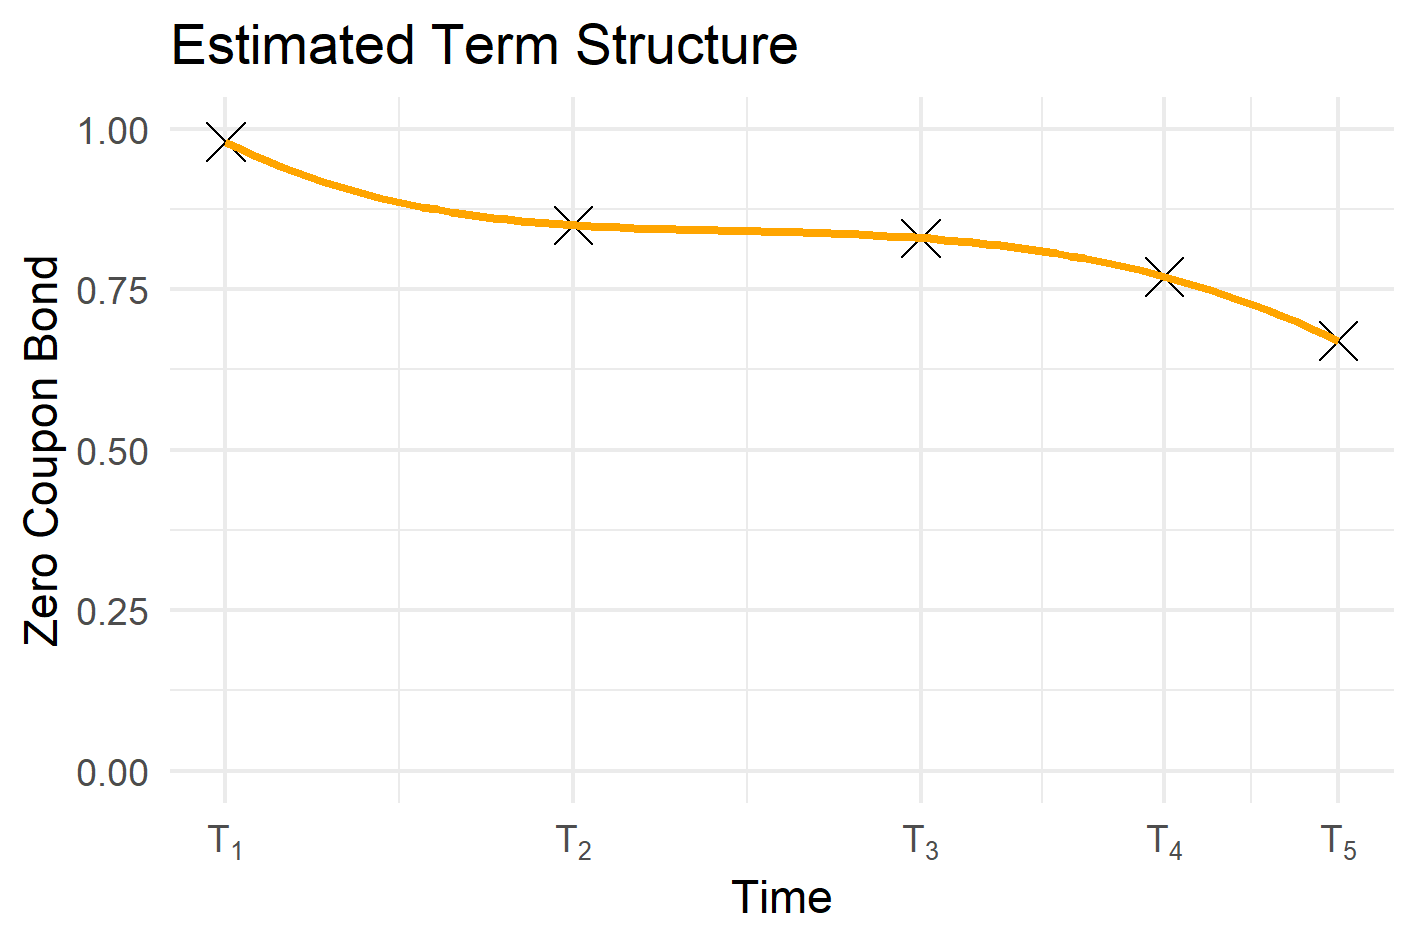
\includegraphics[width=12cm]{figures/Estimating_term_structure.png}
    \caption{Example of estimated term structure}
    \label{fig: Estimaing_term_structure}
\end{figure}


Typical methods to estimate these term structures are regressions and interpolation methods. We will look at parametric estimation methods, in particular, exponential-polynomial families as these methods are often used by central banks. For instance, the Norwegian Central Bank uses the Svensson method \cite{NB_ZCB}.

\subsection{Exponential-Polynomial Families}
Let $P_{1}, \dots, P_{n}$ be the observed ZCB's with maturities $T_{1}, \dots, T_{n}$, the goal will be the followining: 
\[
\min\limits_{\theta}|P_{\theta}(T_{i}) - P_{i}|^{2}
\]

One proposal is the Nelson-Siegel Curve
\begin{align*}
f_{NS}(T, \underbrace{z_{1}, z_{2}, z_{3}, z_{4}}_{\theta}) 
&= 
z_{1} + (z_{2} + z_{3}T)e^{-z_{4}T}
\end{align*}


where one has the following link between $P_{\theta}$ and $f_{NS}$: 
\begin{align*}
P_{\theta}(T) &= \exp\left(
-\int_{0}^{T}f_{NS}(u;\theta)du
\right)    
\end{align*}

The Svensson curve is given by: 
\begin{align*}
f_{S}(T, \theta) &= 
z_{1} + (z_{2}+z_{3}T)e^{-z_{5}T} + z_{4}Te^{-z_{6}T}
\end{align*}






\newpage 
\section{Forward Measures}
Consider the following probability space $(\Omega, \F, (\F_{t})_{t \in [0,T]}, Q))$, furthermore let \\ 
$X\in L^{1}(\Omega, \F, Q)$ as well as $\F_{T}$-measurable. The goal of this section is to study: 
\begin{align*}
\pi(t) &= \E_{Q}\left[
\frac{B(t)}{B(T)}X\bigg{|}\F_{t}
\right]    
\end{align*}

\begin{notation}
We use the following notation: 
\begin{align*}
Z^{T}(t) := \frac{P(t,T)}{P(0,T)B(t)}    
\end{align*}
\end{notation}

\begin{proposition}
\label{prop: Z(T)(t)_Q_martingale}
Assume that $\E_{Q}\left[e^{\frac{1}{2}\int_{0}^{T}\norm{v(s,T)}^{2}ds}\right] < \infty \; \forall T$, then we have that: 
\begin{align*}
Z^{T}(t) 
&= \mathcal{E}_{t}(v(\cdot, T)\bullet W^{Q}), \; t\leq T
\end{align*}
is a $Q$-martingale, furthermore there $\exists\; Q^{T}\sim Q$ such that:
\begin{align*}
\frac{dQ^{T}}{dQ}\bigg{|}_{\F_{t}} = Z^{T}(t)    
\end{align*}
and: 
\begin{align*}
dW^{T}(t) = dW^{Q}(t) - v(t,T)dt    
\end{align*}
defines a $Q^{T}$-Brownian motion. 
\end{proposition}

\begin{proof}
Since we assume that $\E_{Q}\left[e^{\frac{1}{2}\int_{0}^{T}\norm{v(s,T)}^{2}ds}\right] < \infty \; \forall T$, it follows from Novikov's condition (\ref{thm: Novikov_cond_and_implications}) and Theorem $\ref{thm: arbitrage_condition_Q}$, that $Z^{T}(t)$ is a $Q$-martingale. Girsanov's Theorem (\ref{thm: Girsanov's_thm}) justifies that  $\exists\; Q^{T}\sim Q$ such that 
$$
\frac{dQ^{T}}{dQ}\bigg{|}_{\F_{t}} = Z^{T}(t)
$$
and that $dW^{T}(t) = dW^{Q}(t) - v(t,T)dt$ defines a $Q^{T}$-Brownain motion. 
\end{proof}


\begin{proposition}[\textbf{\cite{filipovic2009term}}]
\label{prop: general_option_price}
Let $X \in L^{1}(\Omega, \F, Q)$ as well as $\F_{T}$-measurable, we then have that: 
\[
\E_{Q^{T}}[|X|] < \infty
\]
and: 
\begin{align*}
\pi(t) &= P(t,T)\E_{Q^{T}}[X|\F_{t}]    
\end{align*}
\end{proposition}

\begin{proof}
We get from Bayes theorem (\ref{thm: Bayes_thm}) the following: 
\begin{align*}
\E_{Q^{T}}[|X|] &= \frac{
\E_{Q}\left[|X|\frac{dQ^{T}}{dQ}\right]
}{
\E_{Q}\left[\frac{dQ^{T}}{dQ}\right]
} \\ 
&= 
\frac{
\E_{Q}\left[|X|Z^{T}(T)\right]
}{
Z^{T}(0)
} \\ 
&= 
\E_{Q}\left[
\frac{|X|}{P(0,T)B(T)}
\right] \\
&\leq \E_{Q}[|X|] < \infty
\end{align*}

The second part also relies on Bayes theorem: 
\begin{align*}
\E_{Q^{T}}[X|\F_{t}]
&= 
\frac{
\E_{Q}\left[
X\frac{dQ^{T}}{dQ}\bigg{|}\F_{t}
\right]
}{
\E_{Q}\left[
\frac{dQ^{T}}{dQ}\bigg{|}\F_{t}
\right]
} \\ 
&= 
\frac{
\E_{Q}\left[
XZ^{T}(T)\bigg{|}\F_{t}
\right]
}{
Z^{T}(t)
} \\ 
&\Downarrow \\ 
Z^{T}(t)\E_{Q^{T}}[X|\F_{t}] &= \E_{Q}[XZ^{T}(T)|\F_{t}] \\ 
&\Downarrow \\ 
\pi(t):= P(t,T)\E_{Q^{T}}[X|\F_{t}] &= \E_{Q}\left[
\frac{B(t)}{B(T)}X\bigg{|}\F_{t}
\right]
\end{align*}

\end{proof}


\begin{lemma}[\textbf{\cite{filipovic2009term}}]
\label{lemma: T-discounted-S-discounted-bond}
Let $S>0$ and $S\leq T$. Then the $T$-bond discounted $S$-bond price process:
\begin{align*}
\frac{P(t,S)}{P(t,T)}
&= 
\frac{P(0,S)}{P(0,T)}\mathcal{E}_{t}(\sigma_{S,T}\bullet W^{T}), \;\;t\leq S\leq T
\end{align*}
is a $Q^{T}$-martingale. Where we define: 
\begin{align*}
\sigma_{S,T}(t) &= - \sigma_{T,S}(t) = v(t,S) - v(t,T) = \int_{S}^{T}\sigma(t,u)du    
\end{align*}
Moreover, the $T$- and $S$-forward measures are related by: 
\begin{align*}
\frac{dQ^{S}}{dQ^{T}}\bigg{|}_{\F_{t}}
&= 
\frac{P(t,S)}{P(t,T)}\frac{P(0,T)}{P(0,S)} = \mathcal{E}_{t}(\sigma_{S,T}\bullet W^{T})
\end{align*}
\end{lemma}

\begin{proof}
Quite involved, so we start on the next page: 
\newpage 
\textbf{$Q^{T}$-martingality}: 
\\~\\ 
Let $u\leq t \leq S\leq T$, we then get: 
\begin{align*}
\E_{Q^{T}}\left[
\frac{P(t,S)}{P(t,T)}\bigg{|}\F_{u}
\right] 
&\stackrel{\text{Bayes:\ref{thm: Bayes_thm}}}{=}
\underbrace{\frac{
\E_{Q}\left[
\frac{P(t,S)}{P(t,T)}Z^{T}(T)\bigg{|}\F_{u}
\right]
}{
\E_{Q}\left[
Z^{T}(T)|\F_{u}
\right]
}}_{(*)}
\end{align*}
Now from Proposition \ref{prop: Z(T)(t)_Q_martingale} and the Tower law of conditional expectation (Theorem \ref{thm: Tower_law}), we get that: 
\begin{align*}
(*)
&= 
\frac{
\E_{Q}\left[
\E_{Q}\left[\frac{P(t,S)}{P(t,T)}Z^{T}(T)\bigg{|}\F_{t} \right]
\bigg{|}\F_{u}\right]
}{
Z^{T}(u)
} \\ 
&= 
\frac{
\E_{Q}\left[
\frac{P(t,S)}{P(t,T)}\frac{P(t,T)}{P(0,T)B(t)}
\bigg{|}\F_{u}\right]
}{
\frac{P(u,T)}{P(0,T)B(u)}
} \\ 
&= 
\frac{
\E_{Q}\left[
\frac{P(t,S)}{B(t)}
\bigg{|}\F_{u}\right]
}{
\frac{P(u,T)}{B(u)}
}
= \frac{P(u,S)}{P(u,T)}
\end{align*}
Where the last equality comes from the fact that the discounted zero coupon bond process is a $Q$-martingale.
\\~\\ 
\textbf{Explicit expression:}
\\~\\
From Proposition \ref{prop: Z(T)(t)_Q_martingale}, we have that: 
$P(t,T) = B(t)P(0,T)\mathcal{E}_{t}(v(\cdot, T)\bullet W^{Q})$, this yields: 
\begin{align*}
\frac{P(t,S)}{P(t,T)} 
&= 
\frac{P(0,S)}{P(0,T)}
\frac{
\exp\left(
\int_{0}^{t}v(u,S)dW^{Q}(u) - \frac{1}{2}\int_{0}^{t}\norm{v(u,S)}^{2}du
\right)
}{
\exp\left(
\int_{0}^{t}v(u,T)dW^{Q}(u) - \frac{1}{2}\int_{0}^{t}\norm{v(u,T)}^{2}du
\right)
} \\ 
&= 
\frac{P(0,S)}{P(0,T)}
\exp\left(
\underbrace{
\int_{0}^{t}[v(u,S)-v(u,T)]dW^{Q}(u) 
-\frac{1}{2}\int_{0}^{t}\left(
\norm{v(u,S)}^{2} - \norm{v(u,T)}^{2}
\right)du}_{=(*)}
\right)
\end{align*}
Now: $dW^{Q}(u) = dW^{T}(u) + v(u,T)du$, this leaves us with: 
\begin{align*}
(*) &= \int_{0}^{t}[v(u,S)-v(u,T)]dW^{T}(u) 
+ \int_{0}^{t}[v(u,S)-v(u,T)]v(u,T)du 
-\frac{1}{2}
\int_{0}^{t}\left(
\norm{v(u,S)}^{2}-\norm{v(u,T)}^{2}
\right)du
\end{align*}

\newpage 

Now let's collect the $du$-terms into one integral, and work with the inner expression 
\begin{align*}
&[v(u,S)-v(u,T)]v(u,T) -\frac{1}{2}\left(\norm{v(u,S)}^{2}-\norm{v(u,T)}^{2}\right) \\
=& 
v(u,S)v(u,T)-\norm{v(u,T)}^{2} -\frac{1}{2}\norm{v(u,S)}^{2} + \frac{1}{2}\norm{v(u,T)}^{2} \\ 
=& 
v(u,S)v(u,T)-\frac{1}{2}\norm{v(u,T)}^{2} - \frac{1}{2}\norm{v(u,S)}^{2} \\ 
=& 
-\frac{1}{2}\norm{v(u,S)-v(u,T)}^{2} \\ 
=& -\frac{1}{2}\norm{\sigma_{S,T}(u)}^{2}
\end{align*}
Thus: 
\begin{align*}
\frac{P(t,S)}{P(t,T)}
&= 
\frac{P(0,S)}{P(0,T)}\exp\left(
\int_{0}^{t}\sigma_{S,T}(u)dW^{T}(u) -\frac{1}{2}\int_{0}^{t}\norm{\sigma_{S,T}(u)}^{2}du 
\right) \\ 
&= 
\frac{P(0,S)}{P(0,T)}\mathcal{E}_{t}\left(
\sigma_{S,T}\bullet W^{T}
\right)
\end{align*}

\textbf{Radon-Nikodym derivative:}
\\~\\ 
We have that: 
\begin{align*}
\frac{dQ^{S}}{dQ^{T}}\bigg{|}_{\F_{t}} 
&= 
\frac{dQ^{S}}{dQ}\bigg{|}_{\F_{t}}\bullet\left(
\frac{dQ^{T}}{dQ}\bigg{|}_{\F_{t}}
\right)^{-1} \\ 
&= 
Z^{S}(t)[Z^{T}(t)]^{-1} \\ 
&= 
\frac{P(t,S)}{P(0,S)B(t)}\frac{P(0,T)B(t)}{P(t,T)} \\ 
&= 
\frac{
P(t,S)P(0,T)
}{
P(t,T)P(0,S)
} \\ 
&= 
\mathcal{E}_{t}\left(
\sigma_{S,T}\bullet W^{T}
\right)
\end{align*}
\end{proof}

\newpage 
\section{The LIBOR market model}

\subsection{Introduction}

\begin{definition}[\textbf{LIBOR-rate}]
The LIBOR-rate \nomenclature{LIBOR}{London Interbank Offered Rate} $L(t,T)$ \nomenclature{$L(t,T)$}{LIBOR-rate}
is defined as: 
 \begin{align*}
L(t,T) &= F(t,T,T+\delta) 
= \frac{1}{\delta}\left(
\frac{P(t,T)}{P(t,T+\delta)}-1
\right)     
 \end{align*}
\end{definition}

Typically LIBOR has the following Tenors: 
\begin{itemize}[leftmargin =*]
    \item O/N (Overnight) \nomenclature{O/N}{Overnight}
    \item 1 Week 
    \item 1 Month 
    \item 2 Months 
    \item 3 Months 
    \item 6 Months 
    \item 12 Months
\end{itemize}

The rates are calculated by a trimmed average provided by Panel Banks, meaning that they are based upon expert judgment. Let's say that there were 16 Panel Banks: $B_{1}, \dots, B_{16}$. Each Bank $B_{i}$ would submit a borrowing rate $r_{i}$ to Intercontinental Exchange Benchmark Administration (ICE) \nomenclature{ICE}{Intercontinental Exchange Benchmark Administration}. It would then be sorted, and then one would cut the highest $25\%$, and the lowest $25\%$. For further information, one can consult \cite{ICE_IBA}.  

\begin{example}
Assume that the data below are provided by the Panel Banks for a 3-month tenor. First one collects the data, then sort it in ascending order, followed by trimming the data: 
\begin{align*}
\begin{bmatrix}
0.043 & 0.056 & 0.049 & 0.050\\
0.046 & 0.058 & 0.052 & 0.041 \\ 
0.039 & 0.037 & 0.045 & 0.044 \\ 
0.046 & 0.042 & 0.034 & 0.057
\end{bmatrix}
\to 
\begin{bmatrix}
0.034 & 0.037 & 0.039 & 0.041\\
0.042 & 0.043 & 0.044 & 0.045 \\ 
0.046 & 0.046 & 0.049 & 0.050 \\ 
0.052 & 0.056 & 0.057 & 0.058
\end{bmatrix} 
\to 
\begin{bmatrix}
0.042 & 0.043 & 0.044 & 0.045 \\ 
0.046 & 0.046 & 0.049 & 0.050 
\end{bmatrix} 
\end{align*}

After the data is trimmed one takes the mean: 
\begin{align*}
\frac{1}{8}\left(
0.042 + 0.043 + 0.044 + 0.045 + 0.046 + 0.049 + 0.050
\right)
&= 
0.04550
\end{align*}
One also has conventions for the number of decimals, but these are currency specific. 
\end{example}


\newpage 

In a \textbf{Market model} one is interested in modelling only the relevant $T$'s, meaning that one finds a model for each $T_{i}$. In the market, there are essentially three types of interest rate derivatives: \textbf{caps}, \textbf{floors} and 
\textbf{swaptions}. By swaption, we mean a call/put on a swap.

\begin{definition}[\textbf{LIBOR-Caplet}]
A caplet with reset date \textbf{T} and settlement \textbf{T+$\delta$} pays the holder: LIBOR minus strike $\kappa$ if it is positive: 
\begin{align*}
\delta(F(T;T,T+\delta) -\kappa)^{+} = \delta(L(T,T)-\kappa)^{+}
\end{align*}
\end{definition} 

\begin{definition}[\textbf{LIBOR-Floorlet}]
The opposite of a caplet, it has the following payoff: 
\begin{align*}
\delta(\kappa - L(T,T))^{+}    
\end{align*}
\end{definition}

We assume equidistant times $T_{m} = m\delta, m = 0, 1, \dots, M$, furthermore we will work on: 
$(\Omega, \F, (\F_{t})_{t\in [0,T_{M}]}, Q^{T_{M}})$, $W^{T_{M}}(t)$ is a $Q^{T_{M}}$-BM. In addition $L(0,T_{i})\geq 0 $ are given for $m = 1, \dots, M-1$: 
\begin{align*}
L(0,T_{m}) &= \frac{1}{\delta}\left(
\frac{P(0,T_{m})}{P(0,T_{m+1})}-1
\right), \;\; m = 0, \dots, M-1   
\end{align*}

We get the following timeline:

\begin{tikzpicture}[snake=zigzag, line before snake = 5mm, line after snake = 5mm]
    % draw horizontal line   
    \draw (0,0) -- (2,0);
    \draw[snake] (2,0) -- (4,0);
    \draw (4,0) -- (5,0);
    \draw[snake] (5,0) -- (7,0);
    %\draw[snake] (7,0) -- (9,0);
    \draw (7,0) -- (9,0);

    % draw vertical lines
    \foreach \x in {0,1,2,4,5,7,8}
      \draw (\x cm,3pt) -- (\x cm,-3pt);

    % draw nodes
    \draw (0,0) node[below=3pt] {$ t $} node[above=3pt] {$   $};
    \draw (1,0) node[below=3pt] {$ T_{m} $} node[above=3pt] {$  $};
    \draw (2,0) node[below=3pt] {$ T_{m+1} $} node[above=3pt] {$  $};
    \draw (3,0) node[below=3pt] {$  $} node[above=3pt] {$  $};
    \draw (4,0) node[below=3pt] {$ T_{n} $} node[above=3pt] {$  $};
    \draw (5,0) node[below=3pt] {$ T_{n+1} $} node[above=3pt] {$  $};
    \draw (6,0) node[below=3pt] {$  $} node[above=3pt] {$  $};
    \draw (7,0) node[below=3pt] {$ T_{M-1} $} node[above=3pt] {$ $};
    \draw (8,0) node[below=3pt] {$ T_{M} $} node[above=3pt] {$ $};
  \end{tikzpicture}



The dynamics of $L(t,T_{M-1})$ are given by: 
\begin{align*}
dL(t,T_{M-1}) &= L(t,T_{M-1})\lambda(t,T_{M-1})dW^{T_{M}}(t), \;\; t \leq T_{M-1} \\ 
&\Downarrow \\ 
L(t,T_{M-1}) &= L(0,T_{M-1})\exp\left(
\int_{0}^{t}\lambda(s,T_{M-1})dW^{T_{M}}(s) 
-\frac{1}{2}\int_{0}^{t}\norm{\lambda(s, T_{M-1})}^{2}ds
\right)
\end{align*}

Here: $t \mapsto \lambda(t,T_{M-1})$ is assumed to be an $\R^{d}$-valued bounded deterministic measurable function. 
\\~\\ 
Since
\begin{align*}
\E_{Q^{T_{M}}}\left[
e^{\frac{1}{2}\int_{0}^{T_{M-1}}\norm{\lambda(s,T_{M-1})}^{2}ds}
\right] < \infty 
\;\;\text{and}\;\;
\frac{L(t,T_{M-1})}{L(0,T_{M-1})} = \mathcal{E}_{t}\left(
\lambda(\cdot, T_{M-1})\bullet W^{T_{M}})
\right)
\end{align*}

We have that $L(t,T_{M-1})$ is a $Q^{T_{M}}$-martingale. The idea will be to iterate backwards, so that $L(t,T_{m-1})$ will be martingales under $Q^{T_{m}}$ for $m\geq 2$, we thus need valid measure changes from $Q^{T_{m}}$ to $Q^{T_{m-1}}$ on $\F_{T_{m-1}}$

\newpage

One defines:
\begin{align*}
\frac{
dQ^{T_{M-1}}
}{
dQ^{T_{M}}
}\bigg{|}_{\F_{T_{M-1}}}
&= 
\mathcal{E}_{T_{M-1}}\left(
\sigma_{T_{M-1}, T_{M}}\bullet W^{T_{M}}
\right)
\end{align*}

Where: 
\begin{align*}
\sigma_{T_{M-1}, T_{M}}(t) := 
\frac{
\delta L(t,T_{M-1})
}{
\delta L(t,T_{M-1}) + 1
}
\lambda(t,T_{M-1}), \;t\leq T_{M-1}
\end{align*}

Let $K\in \R$, now as: 
\begin{align*}
\norm{\sigma_{T_{M-1}, T_{M}}(t)}^{2}
&\leq 
\norm{\lambda(t,T_{M-1})}^{2} \leq K \\ 
&\Downarrow \\ 
\E_{Q^{T_{M}}}\left[
e^{
\frac{1}{2}\int_{0}^{T_{M-1}}\norm{\sigma_{T_{M-1}, T_{M}}(s)}^{2}ds
}
\right]
&\leq 
e^{
\frac{1}{2}T_{M-1}K
} < \infty
\end{align*}


Furthermore: 
\begin{align*}
\E_{Q^{T_{M}}}\left[
\frac{
dQ^{T_{M-1}}
}{
dQ^{T_{M}}
}\bigg{|}_{\F_{T_{M-1}}}
\right] 
&= 
\E_{Q^{T_{M}}}\left[
\frac{
dQ^{T_{M-1}}
}{
dQ^{T_{M}}
}\bigg{|}_{\F_{T_{M-1}}}
\bigg{|}\F_{0}
\right] 
=  
\mathcal{E}_{0}\left(
\sigma_{T_{M-1}, T_{M}} \bullet W^{T_{M}}
\right)
= 1
\end{align*}

We thus have that $Q^{T_{M-1}} \sim Q^{T_{M}}$ and from Girsanov's Theorem we have that: 
\begin{align*}
dW^{T_{M-1}}(t) = dW^{T_{M}}(t) - \sigma_{T_{M-1}, T_{M}}(t)dt   
\end{align*}

defines a $Q^{T_{M-1}}$ Brownian Motion on $\F_{T_{M-1}}$. 

\begin{lemma}[\textbf{\cite{filipovic2009term}}]
Let $X$ be a $T_{m}$-contingent claim, we then have that for \\ $t\leq T_{m} \leq T_{n}$ 
\begin{align*}
\frac{\pi(t)}{P(t,T_{m})} 
&= 
\frac{
P(t,T_{n})
}{
P(t,T_{m})
}\E_{Q^{T_{n}}}\left[
\frac{X}{P(T_{m}, T_{n})}
\bigg{|}\F_{t}
\right]
\end{align*}
\end{lemma} 

\begin{proof}
We already have that $\pi(t) = P(t,T_{m})\E_{Q^{T_{m}}}[X|\F_{t}]$, and from 
Lemma \ref{lemma: T-discounted-S-discounted-bond}, by using $S = T_{n}$ and $T = T_{m}$, we have:
\begin{align*}
\frac{
dQ^{T_{m}}
}{
dQ^{T_{n}}
}\bigg{|}_{\F_{t}}
&= 
\mathcal{E}_{t}\left(
\sigma_{T_{m}, T_{n}}\bullet W^{T_{n}}
\right)
\end{align*}

This is a $Q^{T_{n}}$-martingale, now in combination with Bayes Theorem, we get: 
\begin{align*}
\E_{Q^{T_{m}}}\left[
X|\F_{t}
\right]
&= 
\frac{
\E_{Q^{T_{n}}}\left[
\frac{P(T_{m}, T_{m})}{P(T_{m}, T_{n})}
\frac{P(0, T_{n})}{P(0, T_{m})}
\bigg{|}\F_{t}\right]
}{
\frac{P(t, T_{m})}{P(t, T_{n})}
\frac{P(0, T_{n})}{P(0, T_{m})}
} \\ 
&= 
\frac{P(t, T_{n})}{P(t, T_{m})}
\E_{Q^{T_{n}}}\left[
\frac{X}{P(T_{m}, T_{n})}
\bigg{|}\F_{t}\right]
\end{align*}

\end{proof} 

\newpage 

\subsection{LIBOR-caplets}

We will consider a caplet with reset time $T_{n-1}$ and settlement $T_{n}$ and derive the $T_{m}$-price. Meaning that we will be interested in: 
\begin{align*}
Cpl(T_{m}, T_{n-1}, T_{n}) :&= \pi(T_{m}) \\ 
&= 
P(T_{m}, T_{n})\E_{Q^{T_{n}}}\left[
\delta\left(
L(T_{n-1}, T_{n-1}) -\kappa
\right)^{+}
\bigg{|}\F_{T_{m}}
\right]
\end{align*}

\begin{proposition}[\textbf{Price of LIBOR-caplet \cite{filipovic2009term}}]
\begin{align*}
Cpl(T_{m}, T_{n-1}, T_{n})
&= 
\delta P(T_{m}, T_{n})\left[
L(T_{m}, T_{n-1})\Phi(d_{+}(T_{m}, T_{n-1}))
-\kappa \Phi(d_{-}(T_{m}, T_{n-1})
\right]
\end{align*}
where: 
\begin{align*}
d_{\pm}(T_{m}, T_{n-1}) &= 
\frac{
\ln\left( 
\frac{L(T_{m}, T_{n-1})}{\kappa}
\right) \pm 
\frac{1}{2}\int_{T_{m}}^{T_{n-1}}\norm{\lambda(s,T_{n-1})}^{2}ds
}{
\left(
\int_{T_{m}}^{T_{n-1}}\norm{\lambda(s,T_{n-1}}^{2}ds
\right)^{1/2}
}
\end{align*}
\end{proposition}

\begin{proof}
We have the following dynamics for $L(t,T_{n-1})$: 
\begin{align*}
dL(t,T_{n-1}) &= L(t,T_{n-1})\lambda(t,T_{n-1})dW^{T_{n}}(t) 
\end{align*}
where $W^{T_{n}}$ is a $Q^{T_{n}}$-Brownian motion and $t\leq T_{n-1}$
\\~\\ 
We also recall that: 
\begin{align*}
L(t,T_{n-1}) &= L(0,T_{n-1})\mathcal{E}_{t}\left(
\lambda(\cdot, T_{n-1})\bullet W^{T_{n}}
\right) \\ 
L(T_{n-1}, T_{n-1}) &= L(0,T_{n-1})\mathcal{E}_{T_{n-1}}\left(
\lambda(\cdot, T_{n-1})\bullet W^{T_{n}}
\right)
\end{align*}

Leaving us with: 
\begin{align*}
L(T_{n-1}, T_{n-1}) &= L(t,T_{n-1})\mathcal{E}_{t}^{T_{n-1}}\left(
\lambda(\cdot, T_{n-1})\bullet W^{T_{n}}
\right) \\ 
&= L(t,T_{n-1})\exp\left(
\int_{t}^{T_{n-1}}\lambda(s, T_{n-1})dW^{T_{n}}(s)
-\frac{1}{2}\int_{t}^{T_{n-1}}\norm{\lambda(s, T_{n-1}(s)}^{2}ds
\right)
\end{align*} 

We are interested in the $T_{m}$-price, giving us: 
\begin{align*}
L(T_{n-1}, T_{n-1}) &= \underbrace{L(T_{m}, T_{n-1})}_{\text{$\F_{T_{m}}$- measurable}}
\underbrace{\mathcal{E}_{T_{M}}^{T_{n-1}}\left(
\lambda(\cdot, T_{n-1})\bullet W^{T_{n}}
\right)}_{\text{$\F_{T_{m}}$ independent}}    
\end{align*}

Furthermore:
\begin{align*}
\int_{T_{m}}^{T_{n-1}}\lambda(s, T_{n-1})dW^{T_{n}}(s)
\stackrel{Q^{T_{n}}}{\sim} \mathcal{N}\left(
0, \int_{T_{m}}^{T_{n-1}}\norm{\lambda(s,T_{n-1})}^{2}ds
\right)
\end{align*}

Now let $b^{2} = \int_{T_{m}}^{T_{n-1}}\norm{\lambda(s,T_{n-1})}^{2}ds$, and $Z \sim \mathcal{N}(0,1)$, then: 
\begin{align*}
\int_{T_{m}}^{T_{n-1}}\lambda(s, T_{n-1})dW^{T_{n}}(s)
-\frac{1}{2}\int_{T_{m}}^{T_{n-1}}\norm{\lambda(s, T_{n-1}(s)}^{2}ds 
\stackrel{\text{d}}{=} bZ - \frac{1}{2}b^{2}
\end{align*}


This leaves us with: 
\begin{align*}
\E_{Q^{T_{n}}}\left[
(L(T_{n-1}, T_{n-1}) - \kappa)^{+}
\bigg{|}\F_{T_{m}}
\right]
&= 
\E_{Q^{T_{n}}}\left[
\left(x\exp\left(bZ-\frac{1}{2}b^{2}\right) - \kappa
\right)^{+}
\right]_{x = L(T_{n-1}, T_{n-1})}
\end{align*}

\newpage 

\begin{align*}
\left(x\exp\left(bZ-\frac{1}{2}b^{2}\right) - \kappa\right) 
\geq 0 \iff 
Z \geq 
\frac{
\ln\left(\frac{\kappa}{x}\right) + \frac{1}{2}b^{2}
}{
b
}:= d_{1}
\end{align*}

Now this gives us: 
\begin{align*}
\left(x\exp\left(bZ-\frac{1}{2}b^{2}\right) - \kappa
\right)^{+}
&= 
\left(x\exp\left(bZ-\frac{1}{2}b^{2}\right) - \kappa
\right)\mathbbm{1}_{\{Z\geq d_{1}\}}
\end{align*}

Taking the expectation yields: 
\begin{align*}
\E_{Q^{T_{n}}}\left[
\left(x\exp\left(bZ-\frac{1}{2}b^{2}\right) - \kappa
\right)^{+}
\right] &= 
\int_{d_{1}}^{\infty}\left(
x\exp\left(bz-\frac{1}{2}b^{2}
\right) - \kappa
\right)f_{Z}(z)dz \\ 
&= x
\underbrace{
\int_{d_{1}}^{\infty}\exp\left(bz-\frac{1}{2}b^{2}\right)f_{Z}(z)dz 
}_{=(1)}
-\kappa
\underbrace{
\int_{d_{1}}^{\infty}f_{Z}(z)dz
}_{= (2)}
\end{align*}

Let's rewrite $(1)$:
\begin{align*}
(1) = 
\int_{d_{1}}^{\infty}e^{
bz-\frac{1}{2}b^{2}
}\frac{1}{\sqrt{2\pi}}e^{-\frac{z^{2}}{2}}dz   
&= 
\int_{d_{1}}^{\infty}\frac{1}{\sqrt{2\pi}}e^{
-\frac{1}{2}\left(
z^{2} - 2bz + b^{2}
\right)}
dz\\ 
&= 
\int_{d_{1}}^{\infty}\frac{1}{\sqrt{2\pi}}e^{
-\frac{1}{2}\left(
z - b
\right)^{2}}
dz
\end{align*}
This is just an ordinary u-substitution, whit $u = (z-b)$, now 
$z = d_{1}$ gives $u = d_{1}-b = d_{1}'$, so we have: 
\begin{align*}
\int_{d_{1}'}^{\infty}f_{U}(u)du &= P(U\geq d_{1}') 
= P(U\leq -d_{1}') = \Phi(-d_{1}')
\end{align*}

\begin{align*}
d_{+}(T_{m}, T_{n-1}) &:= -d_{1}' = 
\frac{
\ln\left(\frac{x}{\kappa}\right) + \frac{1}{2}\int_{T_{m}}^{T_{n-1}}\norm{\lambda(s,T_{n-1})}^{2}ds
}{
\left(
\int_{T_{m}}^{T_{n-1}}\norm{\lambda(s,T_{n-1})}^{2}ds
\right)^{1/2}
}
\end{align*}

And then we calculate $(2)$:
\begin{align*}
(2) = 
\int_{d_{1}}^{\infty}f_{Z}(z)dz &= P(Z\geq d_{1}) = P(Z \leq -d_{1}) = \Phi(-d_{1})    
\end{align*}
With $-d_{1} = d_{-}(T_{m}, T_{n-1})$. 
\\~\\ 
Plugging all together, yields: 
\begin{align*}
Cpl(T_{m}, T_{n-1}, T_{n}) &= 
P(T_{m}, T_{n})\delta
\E_{Q^{T_{n}}}\left[
\left(x\exp\left(bZ-\frac{1}{2}b^{2}\right) - \kappa
\right)^{+}
\right]_{x = L(T_{n-1}, T_{n-1})} \\ 
&= 
\delta P(T_{m}, T_{n})\left[
L(T_{m}, T_{n-1})\Phi(d_{+}(T_{m}, T_{n-1}))
-\kappa \Phi(d_{-}(T_{m}, T_{n-1})
\right]
\end{align*}

\end{proof}

\chapter{SOFR- Secured Overnight Financing Rate}

\section{Introduction}
Following the LIBOR scandal, the Federal Reserve and regulators in the U.K. have come up with a replacement called the Secured Overnight Financing Rate (SOFR) \nomenclature{SOFR}{Secured Overnight Financing Rate}.
There are also other RFR alternatives (Risk-Free Reference Rates) \nomenclature{RFR}{Risk-Free Reference Rates} who works in a similar way: like SONIA (Sterling Overnight Index Average) 
\nomenclature{SONIA}{Sterling Overnight Index Average} managed by The Bank of England. One could also mention €STR (Euro Short-Term Rate) \nomenclature{€STR}{Euro Short-Term Rate}
\cite{CME_SOFR}
\\~\\
On November.30,2020, the Federal Reserve announced that the LIBOR will be phased out and eventually replaced by June 2023. Banks were also instructed to stop writing contracts using the LIBOR by end of 2021, and that all contracts using the LIBOR should wrap up by June 30, 2023. \cite{hayes_2022}
\\~\\ 
SOFR is fundamentally different from LIBOR. The Federal Reserve Bank of New York collects transaction data from the overnight Treasury Repo market. It then calculates a volume-weighted median interest rate. Which then gets published 08.00 AM (Eastern Time) the following business day \cite{ARRC_SOFR}.
\\~\\ 
This means that SOFR is backward looking as it is based upon overnight transactions, furthermore, it cannot look beyond 24 hours.  
\\~\\
\textbf{Key differences between LIBOR and SOFR/RFR's}

\begin{enumerate}
    \item Calculation Method: LIBOR is calculated based on submissions from Panel Banks. SOFR is based on the overnight repo market. 
    \item Tenors: LIBOR has multiple tenors, while SOFR has one: overnight. Meaning that LIBOR is forward-looking and SOFR is backwards-looking. 
    \item Validity: Following the LIBOR scandal, one has seen that LIBOR has been more prone to manipulation, as one can give higher or lower rate submissions altering the trimmed mean. SOFR is transaction based, meaning that it is harder to manipulate. 
\end{enumerate}

\newpage 

\begin{definition}[\textbf{Discrete overnight SOFR \cite{Skov_2020}}]
The discrete overnight SOFR is defined as:
\[
R_{d_{i}}(T_{i}) = \frac{1}{d_{i}}\left(
\frac{1}{P(T_{i}, T_{i+1})} - 1
\right)
\]
where:
\begin{itemize}[leftmargin=*]
    \item $d_{i}$: denotes the day count fraction multiplied by the number of days to which the overnight rate applies. I.e. $d_{i} = 1/360$ on business days, and $d_{i} = 3/360$ on fridays. 
\end{itemize}
\end{definition}


\begin{figure}[htp]
    \centering
    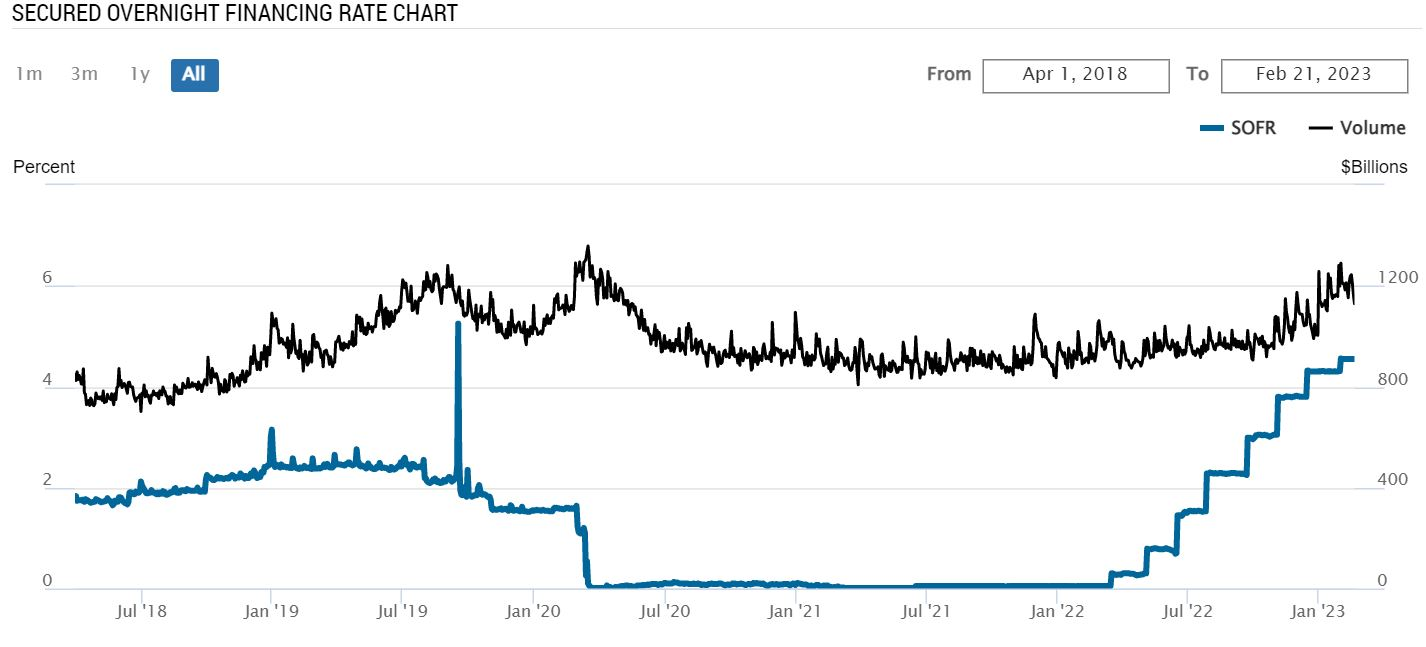
\includegraphics[height = 7cm, width=14cm]{figures/SOFR/overnight_SOFR_Volume.JPG}
    \caption{Overnight SOFR rates. Source: \cite{NewYorkFedSOFR}}
    \label{fig: Overnight_SOFR_rates}
\end{figure}

In this Figure, we see the overnight SOFR rates from April 1, 2018 until February 21, 2023. With corresponding traded volumes. 
\\~\\
We see that there was a spike in September 2019, this was related to quarterly corporate tax payments due September 16. This led to a demand-supply mismatch  \cite{FederalReserve2019}
\\~\\ 
We also see the effect of the pandemic with falling rates around March 2020, until now the rising rates. 


\newpage 

\section{SOFR futures}
Let $(\Omega, \F, (\F_{t})_{t\geq 0}, Q)$ denote our probability space, and let $Q$ be the risk-neutral probability measure defined via the Radon-Nikodym derivative.
\\~\\
\begin{definition}[\textbf{Futures contract \cite{björk2019arbitrage}}]
A futures contract on $X$ with delivery $T$, is a financial asset with following properties: 
\begin{enumerate}[leftmargin =*]
    \item For all $t$ with $0\leq t \leq T$, there exists in the market a quoted object $f(t,T;X)$ known as the futures price of $X$ at time $t$, with delivery $T$. 
    \item At time $T$ of delivery, the holder of the contract pays: $f(T,T;X)$ and receives the claim $X$.
    \item During an arbitrary interval $(s,t]$, the holder of the contract receives: 
    \[
    f(t,T;X) - f(s,T;X)
    \]
\end{enumerate}
\end{definition}

In typical futures contracts, the underlying asset  
$X$ could be oil barrels, corn, cattle etc. In our situation, the underlying asset is an interest rate. The typical settlement is a cash settlement. 
\\~\\ 
\textbf{Some reasons to enter a futures contract:}
\begin{itemize}
    \item Speculation: By trading futures, one can make money by differences in quotes.  
    \item Hedging: One could hedge against higher/lower interest rates. For instance, someone paying a floating rate might buy futures to lock in a future interest rate. 
\end{itemize}



We will be interested in SOFR futures, such futures can be found at CME (Chicago Mercantile Exchange) \nomenclature{CME}{Chicago Mercantile Exchange}. CME uses the following convention for quoting interest rate futures: 
\[
100 - R
\]
Here $R$ will represent the implied SOFR rate. Let's say that we observe a 3M-SOFR futures today with settlement Jun 23, being quoted at $96.6$. This would mean that the implied $3M$-SOFR rate over the period March 23 - June 23 would be: 
\[
(100-96.6)\% = 3.4\% 
\] 
Further specifications on how CME quotes 3M-SOFR futures can be found in  \cite{cmegroup-sofr-futures}. 






\newpage 

When dealing with SOFR futures one distinguishes between 1-month- and 3-month futures, as they are not calculated in the same way:

\begin{definition}[\textbf{SOFR 1-month arithmetic average \cite{Skov_2020}}]
The 1-month \nomenclature{1M}{1-month}
SOFR arithmetic average of the daily reference rate observed over the period $[S,T]$ is defined as: 
\[
R^{1M}(S,T) = \frac{1}{N}\sum_{i=1}^{N}R_{d_{i}}(T_{i})
\]
where:
\begin{itemize}[leftmargin=*]
    \item $N$: total number of days in the month
    \item $S\leq T_{1} \leq \dots \leq T_{N} \leq T$ 
\end{itemize}
\end{definition}

\begin{definition}[\textbf{SOFR 3-month geometric average}]
The 3-month \nomenclature{3M}{3-months}
SOFR geometric average of the daily reference rate observed over the period $[S,T]$ is defined as: 
\[
R^{3M}(S,T) = \frac{1}{T-S}\left(
\prod_{i=1}^{N}(1+d_{i}R_{d_{i}}(T_{i})) - 1
\right)
\]
\end{definition}


As futures contracts are free to enter, we get that: 
\begin{align*}
\E_{Q}\left[
R^{iM}(S,T) - f^{iM}(t,S,T)\bigg{|}\F_{t}
\right] = 0, \;\; i = 1,3   
\end{align*}

Furthermore one uses the following convention: 
\begin{align*}
R^{1M}(S,T) \approx  \frac{1}{T-S}\int_{S}^{T}r(s)ds 
\;\;\text{and}\;\;
R^{3M}(S,T) \approx  \frac{1}{T-S}\left(e^{\int_{S}^{T}r(s)ds} -1\right) 
\end{align*}

This gives arise to the following definitions:

\begin{definition}[\textbf{1-month SOFR futures \cite{Skov_2020}}]
\label{def: 1M_SOFR_futures}
\nomenclature{$f^{1M}(t,S,T)$}{1-month SOFR futures}
We denote the time $t$ rate of the 1-month futures starting to accrue at time $S$ and with settlement on time $T$ as:
\begin{align*}
f^{1M}(t,S,T) &= \frac{1}{T-S}\E_{Q}\left[
\int_{S}^{T}r(s)ds\bigg{|}\F_{t}
\right]    
\end{align*}
\end{definition} 

\begin{definition}[\textbf{3-month SOFR futures \cite{Skov_2020}}]
\label{def: 3M_SOFR_futures}
\nomenclature{$f^{3M}(t,S,T)$}{3-month SOFR futures}
We denote the time $t$ rate of the 3-month futures starting to accrue at time $S$ and with settlement on time $T$ as:  
\begin{align*}
f^{3M}(t,S,T) &= \frac{1}{T-S}\left(
\E_{Q}\left[e^{\int_{S}^{T}r(s)ds}\bigg{|}\F_{t}\right] - 1
\right)    
\end{align*}
\end{definition} 

\newpage 

\begin{proposition}[\textbf{Vasicek dynamics of 1M/3M-SOFR futures}]
Assume that the short rate has the following dynamics: 
\begin{align*}
dr(t) &= \alpha[m-r(t)]dt + \sigma dW^{Q}(t)    
\end{align*}

Then the dynamics of $f^{1M}(t,S,T)$ is given by:
\begin{align*}
df^{1M}(t,S,T) &= \frac{1}{T-S}B(t,S,T)\sigma dW^{Q}(u)
\end{align*}

and the dynamics of $f^{3M}(t,S,T)$ is given by: 
\begin{align*}
df^{3M}(t,S,T) &= \left(
f^{3M}(t,S,T) +\frac{1}{T-S}
\right)B(t,S,T)\sigma dW^{Q}(t)
\end{align*}

Where: 
\begin{align*}
B(t,S,T) &= \frac{1}{\alpha}\left[
e^{-\alpha(S-t)}-e^{\alpha(T-t)}
\right]    
\end{align*}
\end{proposition}


\begin{proof}

From Proposition \ref{prop: Vasicek_ATS}, we have that: 
\begin{align*}
r(s) &= e^{-\alpha(s-t)}r(t) + m[1-e^{-\alpha(s-t)}] + \sigma \int_{t}^{s}e^{-\alpha(s-u)}dW^{Q}(u)
\end{align*}

Now: $f^{1M}(t,S,T) = \frac{1}{T-S}\E_{Q}\left[\int_{S}^{T}r(s)ds|\F_{t} \right]$:  
\begin{align*}
\E_{Q}\left[
r(s)|\F_{t}
\right]
&= 
r(t)e^{-\alpha(s-t)} + m\left(1-e^{-\alpha(s-t)}\right) \\ 
&\Downarrow \\ 
f^{1M}(t,S,T)
&= 
\frac{e^{-\alpha S}- e^{-\alpha T}}{\alpha(T-S)}[r(t)-m]e^{\alpha t}
+ m 
\end{align*}

Giving arise to the following dynamics: 
\begin{align*}
df^{1M}(t,S,T) 
&= 
\frac{e^{-\alpha S}- e^{-\alpha T}}
{\alpha(T-S)}
d\left[
(r(t)-m)e^{\alpha t}
\right]
\end{align*}

Let's work with the differential part first: 
\begin{align*}
d[(r(t)-m)e^{\alpha t}] &= d[r(t)e^{\alpha t}] - md(e^{\alpha t}) \\
&= \alpha me^{\alpha t}dt + \sigma e^{\alpha t}dW^{Q}(t) - \alpha me^{\alpha t}dt \\ 
&= 
\sigma e^{\alpha t}dW^{Q}(t)
\end{align*}

Thus: 
\begin{align*}
df^{1M}(t,S,T) 
&= 
\frac{e^{-\alpha S}- e^{-\alpha T}}
{\alpha(T-S)}\sigma e^{\alpha t}dW^{Q}(t) \\ 
&= \frac{1}{T-S}B(t,S,T)\sigma dW^{Q}(t)
\end{align*}

\newpage 
Now for $f^{3M}(t,S,T)$ we must study $\int_{S}^{T}r(s)ds$:  
\\~\\
We have the following timeline:

\begin{tikzpicture}[snake=zigzag, line before snake = 5mm, line after snake = 5mm]
    % draw horizontal line   
    \draw (0,0) -- (4,0);
    
    % draw vertical lines
    \foreach \x in {0,1,2,3, 4}
      \draw (\x cm,3pt) -- (\x cm,-3pt);

    % draw nodes
    \draw (0,0) node[below=3pt] {$ t $} node[above=3pt] {$   $};
    \draw (1,0) node[below=3pt] {$ S $} node[above=3pt] {$  $};
    \draw (2,0) node[below=3pt] {$ u $} node[above=3pt] {$  $};
    \draw (3,0) node[below=3pt] {$ s $} node[above=3pt] {$  $};
    \draw (4,0) node[below=3pt] {$ T $} node[above=3pt] {$  $};
  \end{tikzpicture}

namely $t\leq S \leq u \leq s \leq T$, this gives us: 
\begin{align*}
\int_{S}^{T}r(s)ds &= \frac{r(t)}{\alpha}\left[
e^{-\alpha(S-t)} - e^{-\alpha(T-t)}
\right]   
+ m(T-S) - \frac{m}{\alpha}\left[
e^{-\alpha(S-t)} - e^{-\alpha(T-t)}
\right] \\ 
&+ 
\sigma 
\underbrace{
\int_{S}^{T}\int_{t}^{s}e^{-\alpha(s-u)}dW^{Q}(u)ds
}_{=(*)}
\end{align*}

Now by additivity of the integral, we see that: 
\begin{align*}
\int_{t}^{s} = \int_{t}^{S} + \int_{S}^{s}    
\end{align*}

This leaves us with: 
\begin{align*}
(*) &= 
\int_{S}^{T}\left(
\int_{t}^{S}e^{-\alpha(s-u)}dW^{Q}(u) + \int_{s}^{S}e^{-\alpha(s-u)}dW^{Q}(u)
\right)ds \\ 
&= 
\underbrace{
\int_{S}^{T}\int_{t}^{S}e^{-\alpha(s-u)}dW^{Q}(u)ds 
}_{=(1)}
+ 
\underbrace{
\int_{S}^{T}\int_{S}^{s}e^{-\alpha(s-u)}dW^{Q}(u)ds
}_{= (2)}
\end{align*}

By Stochastic Fubini, we get: 
\begin{align*}
(1) &= \int_{S}^{T}\int_{t}^{S}e^{-\alpha(s-u)}dW^{Q}(u)ds 
= \int_{t}^{S}\int_{S}^{T}e^{-\alpha(s-u)}dsdW^{Q}(u) 
= (1)'
\end{align*}


\begin{tikzpicture}[snake=zigzag, line before snake = 5mm, line after snake = 5mm]
    % draw horizontal line   
    \draw (0,0) -- (4,0);
    
    % draw vertical lines
    \foreach \x in {0,2,4}
      \draw (\x cm,3pt) -- (\x cm,-3pt);

    % draw nodes
    \draw (0,0) node[below=3pt] {$ S $} node[above=3pt] {$   $};
    \draw (1,0) node[below=3pt] {$  $} node[above=3pt] {$  $};
    \draw (2,0) node[below=3pt] {$ u $} node[above=3pt] {$  $};
    \draw (3,0) node[below=3pt] {$  $} node[above=3pt] {$  $};
    \draw (4,0) node[below=3pt] {$ s $} node[above=3pt] {$  $};
  \end{tikzpicture}


\begin{align*}
\begin{cases}
 S \leq s \leq T \\ 
 S \leq u \leq s
\end{cases}
&\iff
\begin{cases}
 u \leq s \leq T \\ 
 S \leq u \leq T
\end{cases}
\end{align*}

Now this leaves us with: 
\begin{align*}
(2) =\int_{S}^{T}\int_{S}^{s}e^{-\alpha(s-u)}dW^{Q}(u)ds 
=
\int_{S}^{T}\int_{u}^{T}e^{-\alpha(s-u)}dsdW^{Q}(u) = (2)'
\end{align*}

We now calculate the inner integral in $(1)'$ and $(2)'$ respectively: 
\begin{align*}
\int_{S}^{T}e^{-\alpha(s-u)}ds &= \frac{1}{\alpha}\left[
e^{\alpha(S-u)}-e^{-\alpha(T-u)}
\right] \\ 
\int_{u}^{T}e^{-\alpha(s-u)}ds &= \frac{1}{\alpha}\left[
1 -e^{-\alpha(T-u)}
\right]
\end{align*}

We can then define: 
\begin{align*}
\Sigma(u,t,S,T) &= 
    \begin{cases}
      e^{\alpha(S-u)}-e^{-\alpha(T-u)},  & u \in [t,S)\\
      1 -e^{-\alpha(T-u)}, & u\in [S,T]
    \end{cases}
\end{align*}

We are thus left with: 
\begin{align}
\label{eq: Vasicek_closed_expr_3M_SOFR}
\int_{S}^{T}r(s)ds &= \frac{r(t)}{\alpha}\left[
e^{-\alpha(S-t)} - e^{-\alpha(T-t)}
\right]   
+ m(T-S) - \frac{m}{\alpha}\left[
e^{-\alpha(S-t)} - e^{-\alpha(T-t)}
\right] \nonumber \\
&+ \frac{\sigma}{\alpha}\int_{t}^{T}\Sigma(u,t,S,T)dW^{Q}(u)\nonumber \\ 
&= 
\left(
\frac{r(t)-m}{\alpha}
\right)
\left[
e^{-\alpha(S-t)} - e^{-\alpha(T-t)}
\right]
+ m(T-S) 
+ 
\underbrace{
\frac{\sigma}{\alpha}\int_{t}^{T}\Sigma(u,t,S,T)dW^{Q}(u)
}_{\F_{t}-\text{independent}}
\end{align}


As the last part is $\F_{t}$-independent,we get: 
\begin{align*}
\E_{Q}\left[
\exp\left(
\int_{S}^{T}r(s)ds
\right)\bigg{|}\F_{t}
\right] 
&= 
\exp\left[
\left(
\frac{r(t)-m}{\alpha}
\right)
\left[
e^{-\alpha(S-t) - e^{-\alpha(T-t)}}
\right]
+ m(T-S) 
\right] \\
&\times  
\E_{Q}\left[
\exp\left(
\frac{\sigma}{\alpha}\int_{t}^{T}\Sigma(u,t,S,T)dW^{Q}(u)
\right)
\right]
\end{align*}

Since $\Sigma$ is deterministic, we have that: 
\begin{align*}
\E_{Q}\left[
\exp\left(
\frac{\sigma}{\alpha}\int_{t}^{T}\Sigma(u,t,S,T)dW^{Q}(u)
\right)
\right]
&= 
\exp\left(
\frac{1}{2}\frac{\sigma^{2}}{\alpha^{2}}\int_{t}^{T}\Sigma^{2}(u,t,S,T)du
\right)
\end{align*}

This leaves us with the following expression:
\begin{align}
\label{eq: a_hat_3M_SOFR}
 \E_{Q}\left[
\exp\left(
\int_{S}^{T}r(s)ds
\right)\bigg{|}\F_{t}
\right] 
&= 
\exp\left(
A(t,S,T) + B(t,S,T)r(t)
\right):= g(t,r(t))
\end{align}

where: 
\begin{align*}
A(t,S,T) &= m(T-S) - \frac{m}{\alpha}\left[
e^{-\alpha(S-t)} - e^{-\alpha(T-t)}
\right] + \frac{1}{2}\frac{\sigma^{2}}{\alpha^{2}}\int_{t}^{T}\Sigma^{2}(u,t,S,T)du \\
B(t,S,T) &= \frac{1}{\alpha}\left[
e^{-\alpha(S-t)} - e^{-\alpha(T-t)}
\right]
\end{align*}

This means that we have: 
\begin{align}
\label{eq: Vasicek_3M_SOFR_closed_formula}
f^{3M}(t,S,T) &= \frac{1}{T-S}\left[
g(t,r(t)) - 1
\right]    
\end{align}

We note that $\E_{Q}\left[
\exp\left(
\int_{S}^{T}r(s)ds
\right)\bigg{|}\F_{t}
\right]$ is a $Q$-martingale, thus from the Martingale Representation Theorem \ref{thm: Martingale_rep_thm}, we can neglect the dt-terms of $g(t,r(t))$:
\\~\\
We apply Ito's Formula as $g(t,x) \in C^{1,2}([0,\infty]\times \R)$, giving us: 
\begin{align*}
\partial_{t}g(t,x) &= 0, \;\; \partial_{x}g(t,x) = g(t,x)B(t,S,T), \;\; 
\partial_{xx}g(t,x) = g(t,x)B^{2}(t,S,T) \\ 
dr(t)^{2} &= \sigma^{2}dt \\ 
&\Downarrow \\ 
dg(t,r(t)) &= B(t,S,T)g(t,r(t))\sigma dW^{Q}(t)
\end{align*}

\newpage 

This gives the following dynamics for $f^{3M}(t,S,T)$:
\begin{align*}
df^{3M}(t,S,T) &= \frac{1}{T-S}dg(t,r(t)) \\ 
&= \frac{1}{T-S}B(t,S,T)\exp\left(A(t,S,T) + B(t,S,T)r(t)\right)\sigma dW^{Q}(t)\\ 
&= 
\frac{1}{T-S}B(t,S,T)\left[
(T-S)f^{3M}(t,S,T) +1
\right]\sigma dW^{Q}(t) \\ 
&= 
\left(
f^{3M}(t,S,T) + \frac{1}{T-S}
\right)B(t,S,T)\sigma dW^{Q}(t)
\end{align*}
\end{proof}

\newpage 

\section{Interest rate swap with SOFR-futures as floating}


\begin{proposition}
The fixed swap rate $\kappa_{t}^{lM-SOFR}$ in a swap with 1M/3M-SOFR as floating is given by:  
\begin{align*}
 \kappa_{t}^{lM-SOFR} &= 
 \frac{
 \sum_{i=1}^{n}P(t,T_{i})f^{lM}(t,T_{i-1}, T_{i})
 }{
 \sum_{i=1}^{n}P(t,T_{i})
 }, \;\; l = 1,3
\end{align*}
\end{proposition}

\begin{proof}
    
In this swap, we have the following specification, at time $T_{i}$:
\begin{itemize}[leftmargin=*]
    \item Pay $\kappa_{t}^{lM-SOFR}\delta N$ (-)
    \item Receive $f^{kM}(t,T_{i-1}, T_{i})\delta N$, \; l=1,3 (+)
\end{itemize} 

\textbf{Cash flow at time $T_{i}$}:
\begin{align*}
f^{lM}(t, T_{i-1}, T_{i})\delta N - \kappa_{t}^{lM-SOFR}\delta N =
[f^{lM}(t,T_{i-1}, T_{i}) -\kappa_{t}^{lM-SOFR}]\delta N, \;\; l=1,3
\end{align*}

\textbf{Time $t$-value for $t\leq T_{0}$ at time $T_{i}$}: 
\begin{align*}
P(t,T_{i})[f^{lM}(t,T_{i-1}, T_{i}) - \kappa_{t}^{SOFR}]\delta N,\;\; l=1,3
\end{align*}

\textbf{Total payer cash flow:}
\begin{align*}
\mathcal{C}_{P}^{lM-SOFR}(t) &= 
\delta N \sum_{i=1}^{n}P(t,T_{i})[f^{lM}(t,T_{i-1}, T_{i}) - \kappa_{t}^{lM-SOFR}], \;\; l=1,3
\end{align*} 

$\kappa_{t}^{lM-SOFR}$ should be chosen such that: 
\begin{align*}
\E_{Q}[\mathcal{C}_{P}^{lM-SOFR}(t)|\F_{t}] = 0    
\end{align*}

Thus: 
\begin{align*}
\sum_{i=1}^{n}P(t,T_{i})f^{lM}(t,T_{i-1}, T_{i}) &= \sum_{i=1}^{n}P(t,T_{i})\kappa_{t}^{lM-SOFR} \\ 
&\Downarrow \\ 
\kappa_{t}^{lM-SOFR} &= \frac{
\sum_{i=1}^{n}P(t,T_{i})f^{lM}(t,T_{i-1}, T_{i})
}{
\sum_{i=1}^{n}P(t,T_{i})
}
\end{align*}
\end{proof}

\newpage 

Let us consider the case where we look at $l=3$, $n=3$, and $\delta = \frac{3}{12}$. For simplicity, we choose the Vasicek model as this gives an explicit formula for $f^{3M}(t,S,T)$ as described in Equation \ref{eq: Vasicek_3M_SOFR_closed_formula}.

\begin{figure}[htp]
    \centering
    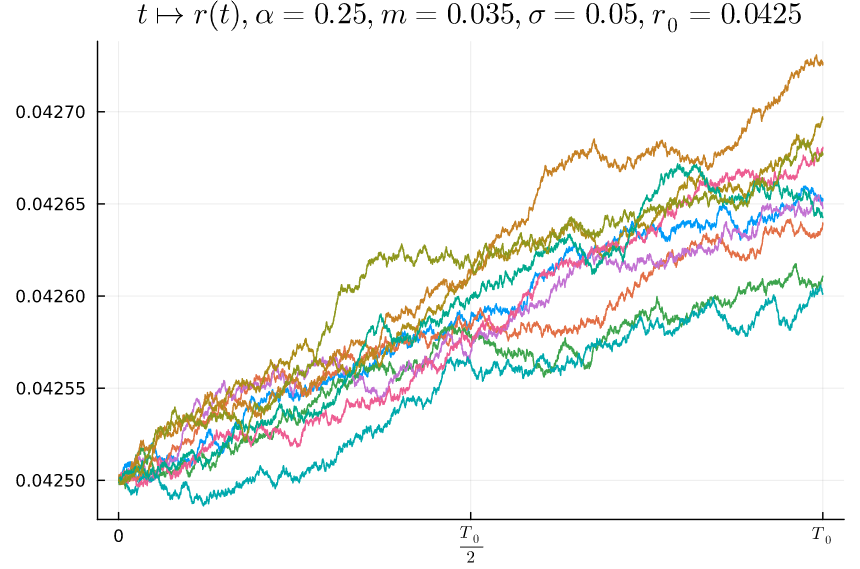
\includegraphics[width=12cm]{figures/SOFR/1M_Vasicek_relaizations.PNG}
    \caption{Realizations of $t \mapsto r(t), t \in [0,T_{0}]$}
    \label{fig: Vasicek_paths}
\end{figure}

Here we see 10 realizations of $[0,T_{0}] \ni t \mapsto r(t)$. In the graph below we see the effect of the time horizon and the starting point for the fixed rate $\kappa_{t}^{3M-SOFR}$:


\begin{figure}[htp]
    \centering
    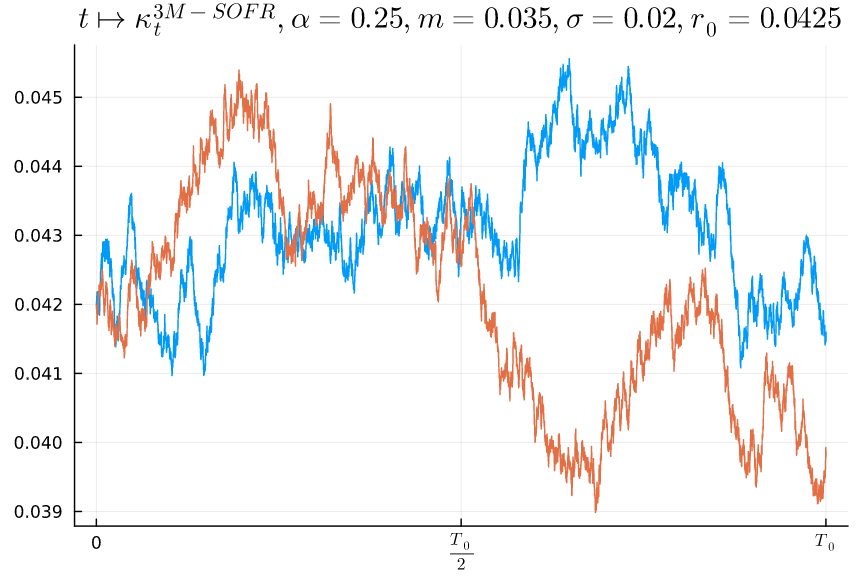
\includegraphics[width=12cm]{figures/SOFR/3M_SOFR_swap_rate_Vasicek.PNG}
    \caption{Realizations of $t \mapsto \kappa_{t}^{3M-SOFR}, t \in [0,T_{0}]$}
    \label{fig: 3M_SOFR_swap_rate}
\end{figure}

Here we took 10 realizations of $[0,T_{0}] \ni t \mapsto \kappa_{t}^{3M-SOFR}$. For $t=0$, we got: 
\begin{align*}
\kappa_{0}^{3M-SOFR} &= 
\frac{
\sum_{i=1}^{3}P(0,T_{i})f^{3M}(0,T_{i-1}, T_{i})
}{
\sum_{i=1}^{3}P(0,T_{i})
}
= 
0.04234
\end{align*}





\newpage 

\section{Options on SOFR futures}

Consider a call option on a SOFR futures, with exercise time $\tau \leq S \leq T$ and strike $\kappa$, the price at time $t \leq \tau$ for $i=1,3$ is given by:
\begin{align*}
C^{iM}(t,\tau) :&= \E_{Q}\left[
\frac{B(t)}{B(\tau)}\left(
f^{iM}(t,S,T) - \kappa
\right)^{+}
\bigg{|}\F_{t}
\right]  
&\stackrel{\text{Prop \ref{prop: general_option_price}}}{=} 
P(t,\tau)\E_{Q^{\tau}}\left[
\left(f^{iM}(t,S,T) - \kappa
\right)^{+}
\bigg{|}\F_{t}
\right]
\end{align*} 

Here we use the convention that $(x)^{+} = \max(x,0)$. From Theorem \ref{thm: arbitrage_condition_Q}, we have: 
\begin{align*}
\frac{dQ^{\tau}}{dQ}\bigg{|}_{\F_{t}} &= \mathcal{E}_{t}(v(\cdot, \tau)\bullet W^{Q})
\end{align*} 

Assuming Novikov's condition holds, i.e: $\E_{Q}\left[e^{\frac{1}{2}\int_{0}^{T}\norm{v(s,\tau)}^{2}ds}\right] < \infty$ we get from Girsanov's theorem, that
\begin{align*}
dW^{\tau}(t) &= dW^{Q}(t) - v(t,\tau)dt    
\end{align*}
defines a $Q^{\tau}$-Brownian motion. 
\\~\\ 
\begin{proposition}[\textbf{1M-SOFR futures Caplet}]
Consider a call option on the 1M-SOFR futures with exercise time $\tau \leq T$ and strike $\kappa$. Let 
\[
df^{1M}(t,S,T) = \Sigma^{1M}(t,S,T)dW^{Q}(t)  
\]
Where $\Sigma^{1M}(t,S,T)$ is assumed to be a deterministic and bounded function. The price at time $t\leq \tau$ is given by: 
\begin{align*}
C^{1M}(t,\tau) &= 
P(t,\tau)\sqrt{
\int_{t}^{\tau}\Sigma^{1M}(u,S,T)^{2}du
}\left[
d\Phi(d) + \varphi(d)
\right]
\end{align*}
Where: 
\begin{align*}
d &= 
\frac{
f^{1M}(t,S,T) + \int_{t}^{\tau}\Sigma^{1M}(u,S,T)v(u,\tau)du - \kappa
}{
\sqrt{
\int_{t}^{\tau}\Sigma^{1M}(u,S,T)^{2}du
}
}
\end{align*}
And $\Phi, \varphi$ represents the cumulative and density function of a standard-normal distribution respectively. 
\end{proposition}

\begin{proof}
The $Q^{\tau}$-dynamics are given by: 
\begin{align*}
df^{1M}(t,S,T) &= 
\Sigma^{1M}(t,S,T)v(t,\tau)dt + \Sigma^{1M}(t,S,T)dW^{\tau}(t)\\ 
&\Downarrow \\ 
f^{1M}(\tau,S,T) &= 
\underbrace{f^{1M}(t,S,T)}_{x} + 
\underbrace{\int_{t}^{\tau}\Sigma^{1M}(u,S,T)v(u,\tau)du}_{m} +  
\int_{t}^{\tau}\Sigma^{1M}(u,S,T)dW^{\tau}(u)
\end{align*}    

Let 
\[
b^{2} = \int_{t}^{\tau}\Sigma^{1M}(u,S,T)^{2}du
\]

We are then left with: 
\begin{align*}
C^{1M}(t,\tau) &= 
\E_{Q^{\tau}}\left[
(f^{1M}(\tau, S,T)-\kappa)^{+}|\F_{t}
\right]    
= 
\E\left[
(x+m+bZ-\kappa)^{+}
\right]\bigg{|}_{x = f^{1M}(t,S,T)}
\end{align*}

where $Z \sim \mathcal{N}(0,1)$, this yields: 

\begin{align*}
\E\left[
(x+m+bZ-\kappa)^{+}
\right]\bigg{|}_{x = f^{1M}(t,S,T)} 
&= 
\int_{\R}(x+m+bz-\kappa)^{+}\varphi(z)dz 
\end{align*}

furthermore: 
\begin{align*}
x + m + bz - \kappa \geq 0 \iff z \geq \frac{\kappa-x-m}{b}:= d'    
\end{align*}

This yields: 
\begin{align*}
\int_{\R}(x+m+bz-\kappa)^{+}\varphi(z)dz  
&= 
\underbrace{
(x+m-\kappa)\int_{d'}^{\infty}\varphi(z)dz
+ b\int_{d'}^{\infty}z\varphi(z)dz
}_{(A)}
\end{align*}

By symmetry of the normal distribution we have: $P(Z > d') = P(Z \leq -d')$, 
where we define: 
\[
d := -d' = \frac{x+m-\kappa}{b}
\]
furthermore $z\varphi(z) = - \varphi'(z)$, thus:

\begin{align*}
\int_{d'}^{\infty}z\varphi(z)dz
&= 
-\int_{d'}^{\infty}\varphi'(z)dz 
= 
-(\varphi(\infty) - \varphi(d'))
= \varphi(d') = \varphi(d)
\end{align*}

Leaving us with:
\begin{align*}
(A) &= (x+m-\kappa)\Phi(d) + b\varphi(d) \\ 
&= b[d\Phi(d) + \varphi(d)]
\end{align*}
Now from Proposition \ref{prop: general_option_price}, we get: 
\begin{align*}
C^{1M}(t,\tau) :&= \pi(t) = P(t,\tau)\E_{Q^{\tau}}\left[
(f^{1M}(\tau, S,T)-\kappa)^{+}|\F_{t}
\right] \\ 
&= 
P(t,\tau)\sqrt{
\int_{t}^{\tau}\Sigma^{1M}(u,S,T)^{2}du
}\left[
d\Phi(d) + \varphi(d)
\right]
\end{align*}
\end{proof}


\newpage 

\section{SOFR hedges}
For SOFR futures we have that there are two approaches for pricing namely arithmetic (1M) and geometric (3M), in this section, we will look at some relationships between them.


\subsection{Hedging 3-month arithmetic with 3-month geometric}
Consider the case where we want to hedge: 
$$
X^{3M_{A}}(S,T) = \frac{1}{T-S}\int_{S}^{T}r_{u}du
$$

Here $[S,T]$ will denote a 3-month period, in the market we only have available
3-month futures $f^{3M}(t,S,T)$  calculated using a geometric mean, this means that our hedge will look like this:

\begin{align*}
\argmin\limits_{a_{t} \in \R}\E_{Q}\left[
\left(
X^{3M_{A}}(S,T)-a_{t}f^{3M}(t,S,T)
\right)^{2}
\bigg{|}\F_{t}
\right]
\end{align*}

Now, fix $t$ and denote
 $G(a_{t}) :=\E_{Q}\left[
\left(X^{3M_{A}}(S,T)-a_{t}f^{3M}(t,S,T)
\right)^{2}
\bigg{|}\F_{t}
\right]
$ 
expanding the square yields:
\begin{align*}
G(a_{t}) &= \E_{Q}\left[(X^{3M_{A}}(S,T))^{2}|\F_{t}\right] -2a_{t}f^{3M}(t,S,T) +
a_{t}^{2}[f^{3M}(t,S,T)]^{2}
\end{align*}
Taking the derivative w.r.t. $a_{t}$ yields: 
\begin{align*}
\frac{d}{da_{t}}G(a_{t}) &= -2f^{3M}(t,S,T) + 2a_{t}[f^{3M}(t,S,T)]^{2}  
\end{align*} 

Now as $\frac{d^{2}}{da_{t}^{2}}G(a_{t}) = 2[f^{3M}(t,S,T)]^{2} > 0$, we have that the minimum is obtained by setting $\frac{d}{da_{t}}G(a_{t}) = 0$:
\begin{align*}
\frac{d}{da_{t}}G(a_{t}) &= 0 \\ 
&\Downarrow \\ 
a_{t} &= \frac{
\E_{Q}[X^{3M_{A}}(S,T)|\F_{t}]
}{
f^{3M}(t,S,T)
} \\ 
&= \frac{
\int_{S}^{T}\E_{Q}[r(u)|\F_{t}]du
}{
(T-S)f^{3M}(t,S,T)
}
\end{align*}

\begin{result}
\label{result: optimal_SOFR_hedge_3MA_vs_3GM}
Considering the above situation, we then have the following:
\begin{align*}
\argmin\limits_{a_{t} \in \R}\E_{Q}\left[
\left(
X^{3M_{A}}(S,T)-a_{t}f^{3M}(t,S,T)
\right)^{2}
\bigg{|}\F_{t}
\right] 
\implies
\hat{a}_{t}^{3M} = \frac{
\int_{S}^{T}\E_{Q}[r(u)|\F_{t}]du
}{
(T-S)f^{3M}(t,S,T)
}
\end{align*}
\end{result} 

\newpage 

\subsection{Affine Term Structure-setting}

\begin{proposition}
Consider the above setting, and let $r = (r_{t})_{t\geq 0}$ be a model that provides ATS, then 
\begin{align*}
\argmin\limits_{a_{t} \in \R}&\E_{Q}\left[
\left(
X^{3M_{A}}(S,T)- a_{t}f^{3M}(t,S,T)
\right)^{2}
\bigg{|}\F_{t}
\right] \\
&\Downarrow \\
\hat{a}_{t} &= \frac{
r(t)(T-S)
+ \int_{S}^{T}\int_{t}^{u}b(s)dsdu 
+ \int_{S}^{T}\int_{t}^{u}\alpha(s)g(s)dsdu
}{
(T-S)f^{3M}(t,S,T)
}
\end{align*}
Where:
\begin{align*}
g(s) &= \exp\left(
\int_{t}^{s}\beta(v)dv
\right)
\left(
\int_{t}^{s}e^{-\int_{t}^{w}\beta(v)dv}b(w)dw + \E_{Q}[r(t)]
\right) 
\end{align*}
\end{proposition}

\begin{proof}
Consider the above setting, but now we assume that $r = (r_{t})_{t\geq 0}$ is a model that provides ATS (Affine Term Structure), now as described in proposition \ref{prop: condition_on_r_ATS}, we have that the dynamics of $r$ can be written as: 
\begin{align*}
dr(t) &= [b(t) + \beta(t)r(t)]dt + \sqrt{a(t) + \alpha(t)r(t)}dW^{Q}(t)
\end{align*}
Here $b, \beta, a, \alpha$ are deterministic continuous functions. Now from the dynamics, we get that for $u\geq t$: 
\begin{align*}
r(u) &= r(t) + \int_{t}^{u}b(s)ds + \int_{t}^{u}[\beta(s)r(s)]ds
+ \int_{t}^{u}\sqrt{\alpha(s)}dW^{Q}(s)
+ \int_{t}^{u}\sqrt{\alpha(s)r(s)}dW^{Q}(s)
\end{align*}

Each term is assumed to be Ito-integrable, i.e in $M^{2}([0,T])$, and by \\ $\F_{t}$-independence, we get:
\begin{align*}
\E_{Q}\left[
\int_{t}^{u}\sqrt{\alpha(s)}dW^{Q}(s)
\right]
&= 0 \\ 
\E_{Q}\left[
\int_{t}^{u}\sqrt{\alpha(s)r(s)}dW^{Q}(s)
\right] 
&= 0
\end{align*} 

And by using Stochastic-Fubini(\ref{thm: Stochastic_Fubini}), we get:
\begin{align*}
\E_{Q}\left[
\int_{t}^{u}[\beta(s)r(s)]ds
\right]
&= 
\int_{t}^{u}\beta(s)\E_{Q}[r(s)]ds
\end{align*}

This leaves us with: 
\begin{align*}
\int_{S}^{T}\E_{Q}[r(u)|\F_{t}]du 
&= r(t)(T-S)
+ \int_{S}^{T}\int_{t}^{u}b(s)dsdu 
+ \int_{S}^{T}\int_{t}^{u}\alpha(s)\E_{Q}[r(s)]dsdu
\end{align*}


\textbf{Overview of time-interval:}


\begin{tikzpicture}[snake=zigzag, line before snake = 5mm, line after snake = 5mm]
    % draw horizontal line   
    \draw (0,0) -- (9,0);
    %\draw[snake] (2,0) -- (4,0);
    %\draw (4,0) -- (5,0);
    %\draw[snake] (5,0) -- (7,0);
    %\draw[snake] (7,0) -- (9,0);
    %\draw (9,0) -- (10,0);

    % draw vertical lines
    \foreach \x in {0,2,4,5,7}
      \draw (\x cm,3pt) -- (\x cm,-3pt);

    % draw nodes
    \draw (0,0) node[below=3pt] {$ t $} node[above=3pt] {$   $};
    %\draw (1,0) node[below=3pt] {$ T_{0} $} node[above=3pt] {$  $};
    \draw (2,0) node[below=3pt] {$ S $} node[above=3pt] {$  $};
    %\draw (3,0) node[below=3pt] {$  $} node[above=3pt] {$  $};
    \draw (4,0) node[below=3pt] {$ s $} node[above=3pt] {$  $};
    \draw (5,0) node[below=3pt] {$ u $} node[above=3pt] {$  $};
    \draw (6,0) node[below=3pt] {$  $} node[above=3pt] {$  $};
    \draw (7,0) node[below=3pt] {$ T $} node[above=3pt] {$ $};
    %\draw (9,0) node[below=3pt] {$ T_{M} $} node[above=3pt] {$ $};
\end{tikzpicture} 
  
Thus in our setting we have: $t\leq S \leq s \leq u \leq T$, using same argument as above: 

\begin{align*}
r(s) &= r(t) + \int_{t}^{s}b(v)dv + \int_{t}^{s}[\beta(v)r(v)]dv
+ \int_{t}^{s}\sqrt{\alpha(v)}dW^{Q}(v)
+ \int_{t}^{s}\sqrt{\alpha(v)r(v)}dW^{Q}(v)    
\end{align*}

Now let $g(s) := \E_{Q}[r(s)]$: 
\begin{align*}
g(s) &= r(t) + \int_{t}^{s}b(v)dv + \int_{t}^{s}\beta(v)\E_{Q}[r(v)]dv
\end{align*}

Now taking the derivative w.r.t. $s$ and using the fundamental theorem of calculus, we get: 
\begin{align*}
g'(s) &= b(s) + \beta(s)\E_{Q}[r(s)] \\ 
&= b(s) + \beta(s)g(s), \; g(t) = \E_{Q}[r(t)]
\end{align*}

This is an ordinary differential equation, with the explicit solution given by:
\begin{align*}
 g(s) &= \exp\left(
 \int_{t}^{s}\beta(v)dv
 \right)
 \left(
 \int_{t}^{s}e^{-\int_{t}^{w}\beta(v)dv}b(w)dw + \E_{Q}[r(t)]
 \right)
\end{align*}
\end{proof}


\subsection{Hedging with available instruments in the market}

We now denote: 
\begin{align*}
X^{3M_{A}}(S,T) &= \frac{1}{T-S}\int_{S}^{T}r_{u}du = \frac{1}{T-S}Z(S,T) \\ 
f^{3M_{A}}(t,S,T) &= \frac{1}{T-S}\E_{Q}\left[
\int_{S}^{T}r_{u}du
\right] = \frac{1}{T-S}\E_{Q}[Z(S,T)|\F_{t}]
\end{align*}

Now from Jensen's Inequality \ref{thm: Jensen's_ineuality}, we have that for $Z, \varphi(Z) \in L^{1}(\Omega, \F, Q)$, with $\varphi(x) = e^{x}$
\begin{align}
\label{eq: hedging_availible_inst_market_1}
\exp\left(
\E_{Q}[Z(S,T)|\F_{t}]
\right)
&\leq 
\E_{Q}\left[
\exp(Z(S,T))|\F_{t}
\right] \nonumber \\ 
&\Updownarrow \nonumber \\ 
\exp\left(
(T-S)f^{3M_{A}}(t,S,T)
\right) 
&\leq 
\E_{Q}\left[\exp(Z(S,T))|\F_{t}\right]
\end{align} 

Now from definition \ref{def: 3M_SOFR_futures}, we have: 
\begin{align}
\label{eq: hedging_availible_inst_market_2}
f^{3M}(t,S,T) &= \frac{1}{T-S}\left(
\E_{Q}\left[
\underbrace{e^{\int_{S}^{T}r_{u}du}}_{e^{Z}}
\bigg{|}\F_{t}\right] - 1
\right) \nonumber \\ 
&\Downarrow \nonumber \\ 
\E_{Q}[\exp(Z(S,T))|\F_{t}] &= (T-S)f^{3M}(t,S,T) + 1
\end{align}

Now by inserting \ref{eq: hedging_availible_inst_market_2} into \ref{eq: hedging_availible_inst_market_1} yields:

\begin{align*}
\exp\left(
(T-S)f^{3M_{A}}(t,S,T)
\right) 
&\leq 
(T-S)f^{3M}(t,S,T) + 1 \\ 
&\Updownarrow \\
f^{3M_{A}}(t,S,T) &\leq 
\frac{
\ln[(T-S)f^{3M}(t,S,T)]
}{
(T-S)
}
\end{align*}

\newpage 

\subsection{Hedging three-month arithmetic with 1M-SOFR futures}
\label{sec: 3M_A_vs_(a,b,c)_1M_SOFR}
We still want to hedge: 
$$
X^{3M_{A}}(S,T) = \frac{1}{T-S}\int_{S}^{T}r_{u}du
$$

However, now we will not use the available 3M-SOFR future contract, rather we will hedge by buying $(\hat{a}_{t}, \hat{b}_{t}, \hat{c}_{t})$ 1M-SOFR future contracts at time $t$. Here $[S,T]$ will still denote a 3M period, we get the following timeline:


\begin{tikzpicture}[snake=zigzag, line before snake = 5mm, line after snake = 5mm]
    % draw horizontal line   
    \draw (0,0) -- (8,0);
    %\draw[snake] (2,0) -- (4,0);
    %\draw (4,0) -- (6,0);
    %\draw[snake] (6,0) -- (8,0);
    %\draw (8,0) -- (9,0);
    % Calligraphic brace
    \draw [
    decorate, 
    decoration = {calligraphic brace,
                  raise=5pt,
                  amplitude=5pt,
                  aspect=0.50}] (1,0) --  (7.0,0)
                  node[pos=0.50, above =1 0pt,black]{$3M$};

    % draw vertical lines
    \foreach \x in {0,1.0,3.0,5.0,7.0}
      \draw (\x cm,3pt) -- (\x cm,-3pt);

    % draw nodes
    \draw (0,0) node[below=3pt] {$ t $} node[above=3pt] {$   $};
    \draw (1,0) node[below=3pt] {$ S $} node[above=3pt] {$  $};
    \draw (3.0,0) node[below=3pt] {$ T_{1M} $} node[above=3pt] {$  $};
    \draw (5.0,0) node[below=3pt] {$ T_{2M} $} node[above=3pt] {$  $};
    \draw (7.0,0) node[below=3pt] {$ T $} node[above=3pt] {$   $};
  \end{tikzpicture}

Our hedge will in this case look like: 
\begin{align*}
\argmin\limits_{(a_{t}, b_{t}, c_{t})\in \R^{3}}\E_{Q}\left[
\left(
X^{3M_{A}}(S,T)- \left[
a_{t}f^{1M}(t,S,T_{1M}) + 
b_{t}f^{1M}(t,T_{1M}, T_{2M}) + 
c_{t}f^{1M}(t,T_{2M}, T)
\right]
\right)^{2}
\bigg{|}\F_{t}
\right]
\end{align*}

Denote: 
\begin{align*}
G(a_{t}, b_{t}, c_{t}) := 
\E_{Q}\left[
\left(
X^{3M_{A}}(S,T)- \left[
a_{t}f^{1M}(t,S,T_{1M}) + 
b_{t}f^{1M}(t,T_{1M}, T_{2M}) + 
c_{t}f^{1M}(t,T_{2M}, T)
\right]
\right)^{2}
\bigg{|}\F_{t}
\right]
\end{align*} 

Expanding the square yields: 
\begin{align*}
G(a_{t}, b_{t}, c_{t}) 
&= 
\E_{Q}\left[(X^{3M_{A}}(S,T))^{2}|\F_{t} \right] \\
&-2\E_{Q}[X^{3M_{A}}(S,T)|\F_{t}]\left[
a_{t}f^{1M}(t,S,T_{1M}) + 
b_{t}f^{1M}(t,T_{1M}, T_{2M}) + 
c_{t}f^{1M}(t,T_{2M}, T)
\right] \\ 
&+ a_{t}^{2}[f^{1M}(t,S,T_{1M})]^{2} \\ 
&+ 2a_{t}f^{1M}(t,S,T_{1M})\left[
b_{t}f^{1M}(t,T_{1M}, T_{2M}) + 
c_{t}f^{1M}(t,T_{2M}, T)
\right] \\ 
&+ b_{t}^{2}[f^{1M}(t,T_{1M}, T_{2M})]^{2} \\ 
&+ 2b_{t}c_{t}\left[
f^{1M}(t,T_{1M}, T_{2M})f^{1M}(t,T_{2M}, T)
\right] \\ 
&+ c_{t}^{2}[f^{1M}(t,T_{2M}, T)]^{2}
\end{align*} 

Fix $t$, to ease the notation we denote $(a_{t}, b_{t}, c_{t}) = (x_{1}(t), x_{2}(t), x_{3}(t)) = \mathbf{x}_{t}$ furthermore let: 
\[
\left(
f^{1M}(t,S,T_{1M}),f^{1M}(t,T_{1M}, T_{2M}), f^{1M}(t,T_{2M}, T) 
\right)
= \left(
\alpha_{t}, \beta_{t}, \gamma_{t}
\right)
\]
We also let: 
\begin{align*}
\E_{Q}\left[(X^{3M_{A}}(S,T))^{2}|\F_{t} \right] &= p_{t} \\ 
\E_{Q}[X^{3M_{A}}(S,T)|\F_{t}] &= q_{t}
\end{align*}

This leaves us with: 
\begin{align*}
G(\mathbf{x}_{t}) &= 
p_{t} \\
&- 2q_{t}\left[
\alpha_{t} x_{1}(t) + \beta_{t} x_{2}(t) + \gamma_{t} x_{3}(t)
\right] \\ 
&+ \alpha_{t}^{2}x_{1}(t)^{2} \\ 
&+ 2\alpha x_{1}(t)\left[
\beta_{t} x_{2}(t) + \gamma_{t} x_{3}(t)
\right] \\ 
&+ \beta_{t}^{2}x_{2}(t)^{2} \\ 
&+ 2\beta_{t}\gamma_{t} x_{2}(t)x_{3}(t) \\ 
&+ \gamma_{t}^{2}x_{3}(t)^{2}
\end{align*}


\newpage 
To get a bit better grasp of $G(\mathbf{x}_{t})$ we include a level plot:

\begin{figure}[htp]
    \centering
    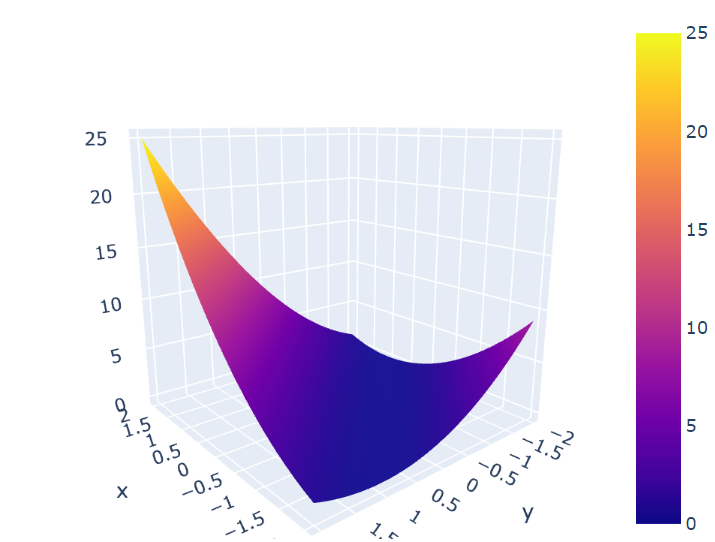
\includegraphics[width=12cm]{figures/SOFR/plot_G(x)_special_case.PNG}
    \caption{level Curve $G(\mathbf{x}_{t}) = k$, where all constants are set to one}
    \label{fig: plot_G(x)_SOFR_1M}
\end{figure}

\textbf{NB!} Figure \ref{fig: plot_G(x)_SOFR_1M}, is purely for illustration purposes, this will not be a realistic representation of $G(\mathbf{x}_{t})$. 
\\~\\
We will be interested in obtaining a minimum of $G(\mathbf{x}_{t})$, meaning that we will be interested in the following:  

\begin{align*}
\nabla G(\mathbf{x}_{t}) &= 
\left(
\partial_{x_{1}}G(\mathbf{x}_{t}), 
\partial_{x_{2}}G(\mathbf{x}_{t}), 
\partial_{x_{3}}G(\mathbf{x}_{t})
\right) 
\end{align*}

Where: 
\begin{align*}
\partial_{x_{1}}G(\mathbf{x}_{t}) &= 
-2q_{t}\alpha_{t} 
+ 2 \alpha_{t}^{2}x_{1}(t)  
+ 2\alpha_{t}\left[
\beta_{t} x_{2}(t)+ \gamma_{t} x_{3}(t)
\right] \\ 
\\
\partial_{x_{2}}G(\mathbf{x}_{t}) &=
-2q_{t}\beta_{t}
+ 2\beta_{t}^{2} x_{2}(t)
+ 2\beta_{t}\left[
\alpha_{t} x_{1}(t) + \gamma_{t} x_{3}(t)
\right] \\ 
\\ 
\partial_{x_{3}}G(\mathbf{x}_{t}) &=
-2q_{t}\gamma_{t}
+ 2\gamma_{t}^{2}x_{3}(t)
+ 2\gamma_{t}\left[
\alpha_{t} x_{1}(t) + \beta_{t} x_{2}(t)
\right]
\end{align*}

In order to verify that $G$ obtains a minimum we need the Hessian matrix $H(G)$ of $G$. This will be a $3\times 3$ matrix with entries:  

\begin{align*}
[H(G)]_{i,j} &= 
\frac{
\partial^{2}G
}{
\partial x_{i}\partial x_{j}
}, \; i=1,2,3,\;j=1,2,3
\end{align*}

Meaning that our Hessian matrix looks the following:
\begin{align*}
H(G) &= 
\begingroup
\renewcommand*{\arraystretch}{1.5}
\begin{bmatrix}
2\alpha_{t}^{2} & 
2\alpha_{t} \beta_{t} & 
2\alpha_{t} \gamma_{t} \\ 
2\alpha_{t} \beta_{t} &
2\beta_{t}^{2} &
2\beta_{t} \gamma_{t} \\
2\alpha_{t} \gamma_{t} &
2\beta_{t} \gamma_{t} & 
2\gamma_{t}^{2}
\end{bmatrix}
\endgroup
\end{align*}


Now as $\frac{\partial^{2}G(\mathbf{x}) }{\partial x_{i}^{2}} > 0$ for $i=1,2,3$ we know that the minimum should be obtained by setting $\partial_{x_{i}}G(\mathbf{x}) = 0$, i.e we must solve: 
\begin{align}
\label{eq: partial_derivative_equal_zero}
\nabla G(\mathbf{x}_{t}) = \mathbf{0}    
\end{align}

Now Equation \ref{eq: partial_derivative_equal_zero}, gives arise to the following matrix equation: 
\begin{align*}
\underbrace{
\begin{bmatrix}
\alpha_{t}^{2} & \alpha_{t}\beta_{t} & \alpha_{t}\gamma_{t} \\ 
\beta_{t}^{2} & \alpha_{t}\beta_{t} & \beta_{t}\gamma_{t} \\ 
\gamma_{t}^{2} & \alpha_{t}\gamma_{t} & \beta_{t}\gamma_{t}
\end{bmatrix}
}_{M}
\underbrace{
\begin{bmatrix}
x_{1}(t) \\ 
x_{2}(t) \\ 
x_{3}(t)
\end{bmatrix}
}_{\mathbf{x}_{t}}
&= 
\underbrace{
q 
\begin{bmatrix}
\alpha_{t} \\ 
\beta_{t} \\ 
\gamma_{t} 
\end{bmatrix}
}_{\mathbf{b}}
\iff  
M\mathbf{x}_{t} = \mathbf{b}
\end{align*}

Now: 
\begin{align*}
\det(M) &= 
\alpha_{t}^{2}\left[
\alpha_{t}\beta_{t}^{2}\gamma_{t} - \alpha_{t}\beta_{t}\gamma_{t}^{2}
\right]
- \alpha_{t}\beta_{t}\left[
\beta_{t}^{3}\gamma_{t} - \beta_{t}\gamma_{t}^{3}
\right]
+ \alpha_{t}\gamma_{t}\left[
\beta_{t}^{2}\alpha_{t}\gamma_{t} -\alpha_{t}\beta_{t}\gamma_{t}^{2}
\right] \\ 
&= 
\alpha_{t}\beta_{t}\gamma_{t}(\beta_{t}-\gamma_{t})\left[
\alpha_{t}(\alpha_{t}+\gamma_{t}) -\beta_{t}(\beta_{t} + \gamma_{t})
\right]
\end{align*}

In order for $\det(M) \neq 0$, we must have:
\begin{empheq}[box=\fbox]{align}
\alpha_{t} &\neq 0, \; \beta_{t} \neq 0, \; \gamma_{t} \neq 0  \nonumber
\\
\beta_{t} &\neq \gamma_{t}, \; \gamma_{t} \neq -(\alpha_{t} + \beta_{t}) \label{eq: condition_det(M)_not_zero}
\end{empheq}

%Assume that the necessary conditions in \ref{eq: condition_det(A)_not_zero} holds, we then get, that the inverse is %given by: 

\begin{comment}
\begin{align*}
M^{-1} &= 
\begingroup
\renewcommand*{\arraystretch}{3.0}
\begin{bmatrix}
\frac{
\beta -\gamma
}{
(\alpha - \beta)[\alpha\beta - \alpha\gamma + \beta^{2}-\gamma^{2}]
}
& 
\frac{
-\beta^{2}+\alpha\gamma
}{
\beta(\alpha -\beta)[\alpha\beta - \alpha\gamma + \beta^{2}-\gamma^{2}]
}
& 
-\frac{
1
}{
\alpha\beta -\alpha\gamma + \beta^{2}-\gamma^{2}
} \\
\frac{
-\beta^{2}+\gamma
}{
\alpha(\alpha-\beta)[\alpha\beta -\alpha\gamma +\beta^{2}-\gamma^{2}]
}
& 
\frac{
\alpha\beta -\gamma^{2}
}{
\beta(\alpha-\beta)[\alpha\beta -\alpha\gamma +\beta^{2}-\gamma^{2}]
}
& 
-\frac{
1
}{
\alpha\beta -\alpha\gamma +\beta^{2}-\gamma^{2}
} \\ 
\frac{
\beta-\gamma
}{
(\alpha -\beta)[\alpha\beta -\alpha\gamma + \beta^{2}-\gamma^{2}]
} 
& 
\frac{
\alpha^{2}-\beta\gamma
}{
\beta(\alpha-\beta)[\alpha\beta - \alpha\gamma + \beta^{2}-\gamma^{2}]
}
&
\frac{
\alpha + \beta
}{
\gamma[\alpha\beta -\alpha\gamma + \beta^{2} - \gamma^{2}]
}
\end{bmatrix}
\endgroup
\end{align*}
\end{comment}

Thus the optimal weight $\hat{\mathbf{x}}_{t}$ will then be:   
\begin{align*}
\hat{\mathbf{x}}_{t} &= 
M^{-1}\mathbf{b}
\end{align*}


Now if the Condition \ref{eq: condition_det(M)_not_zero} does not hold, one approach could be:

\begin{align}
\label{eq: Basis_Pursuit_lp}
\begin{array}{ll@{}ll}
\text{minimize}  & \displaystyle\sum\limits_{i=1}^{3}x_{i}(t)&  &\\
\text{subject to}& \displaystyle   M\mathbf{x}_{t} = & \mathbf{b}
\end{array}    
\end{align}

Assume that $\Tilde{\mathbf{x}}_{t}$ is the optimal solution to \ref{eq: Basis_Pursuit_lp}, this method is
very much related to Basis Pursuit \cite{chen1998atomic}.



\newpage 

\subsection{Simulation of Error distribution}

In order to say something about how good the hedge is in Result \ref{result: optimal_SOFR_hedge_3MA_vs_3GM}, we study: 
\begin{align*}
ER_{1}(t) :&= X^{3M_{A}}(S,T) - \hat{a}_{t}^{3M}f^{3M}(t,S,T) \\ 
&= \frac{1}{T-S}\int_{S}^{T}r(u)du - \frac{1}{T-S}\int_{S}^{T}\E_{Q}[r(u)|\F_{t}]du \\ 
&= 
\frac{1}{T-S}\left(
\int_{S}^{T}r(u)du - \int_{S}^{T}\E_{Q}[r(u)|\F_{t}]du
\right)
\end{align*}

We will also study the Error distribution from Section \ref{sec: 3M_A_vs_(a,b,c)_1M_SOFR}, now this will correspond to: 
\begin{align*}
ER_{2}(t) &= 
X^{3M_{A}}(S,T) - \left(
\hat{a}_{t}f^{1M}(t,S,T_{1M}) + 
\hat{b}_{t}f^{1M}(t,T_{1M}, T_{2M}) + 
\hat{c}_{t}f^{1M}(t,T_{2M}, T)
\right)
\end{align*}


We choose the Vasicek model for simulation:
\begin{align*}
dr(t) &= \alpha[m-r(t)]dt + \sigma dW^{Q}(t)    
\end{align*}

For calculating $X^{3M_{A}}(S,T)$, we use the closed expression for $\int_{S}^{T}r(u)du$  as described in Equation \ref{eq: Vasicek_closed_expr_3M_SOFR} p.\pageref{eq: Vasicek_closed_expr_3M_SOFR}:

\begin{align*}
\int_{S}^{T}r(u)du 
&= 
\left(
\frac{r(t)-m}{\alpha}
\right)
\left[
e^{-\alpha(S-t)} - e^{-\alpha(T-t)}
\right]
+ m(T-S) 
+ 
\frac{\sigma}{\alpha}\int_{t}^{T}\Sigma(u,t,S,T)dW^{Q}(u)
\end{align*}

Where: 
\begin{align*}
\Sigma(u,t,S,T) &= 
\left[
e^{-\alpha(S-u)}-e^{-\alpha(T-u)}
\right]\mathbbm{1}_{[t,S)}(u) 
+ 
\left[
1-e^{-\alpha(T-u)}
\right]\mathbbm{1}_{[S,T]}(u)
\end{align*}


For simplicity we fix $t=0$, meaning that we will study: 
$ER_{1}(0)$ and $ER_{2}(0)$, using the Vasicek model, where the parameters are as shown below:

\begin{figure}[htp]
    \centering
    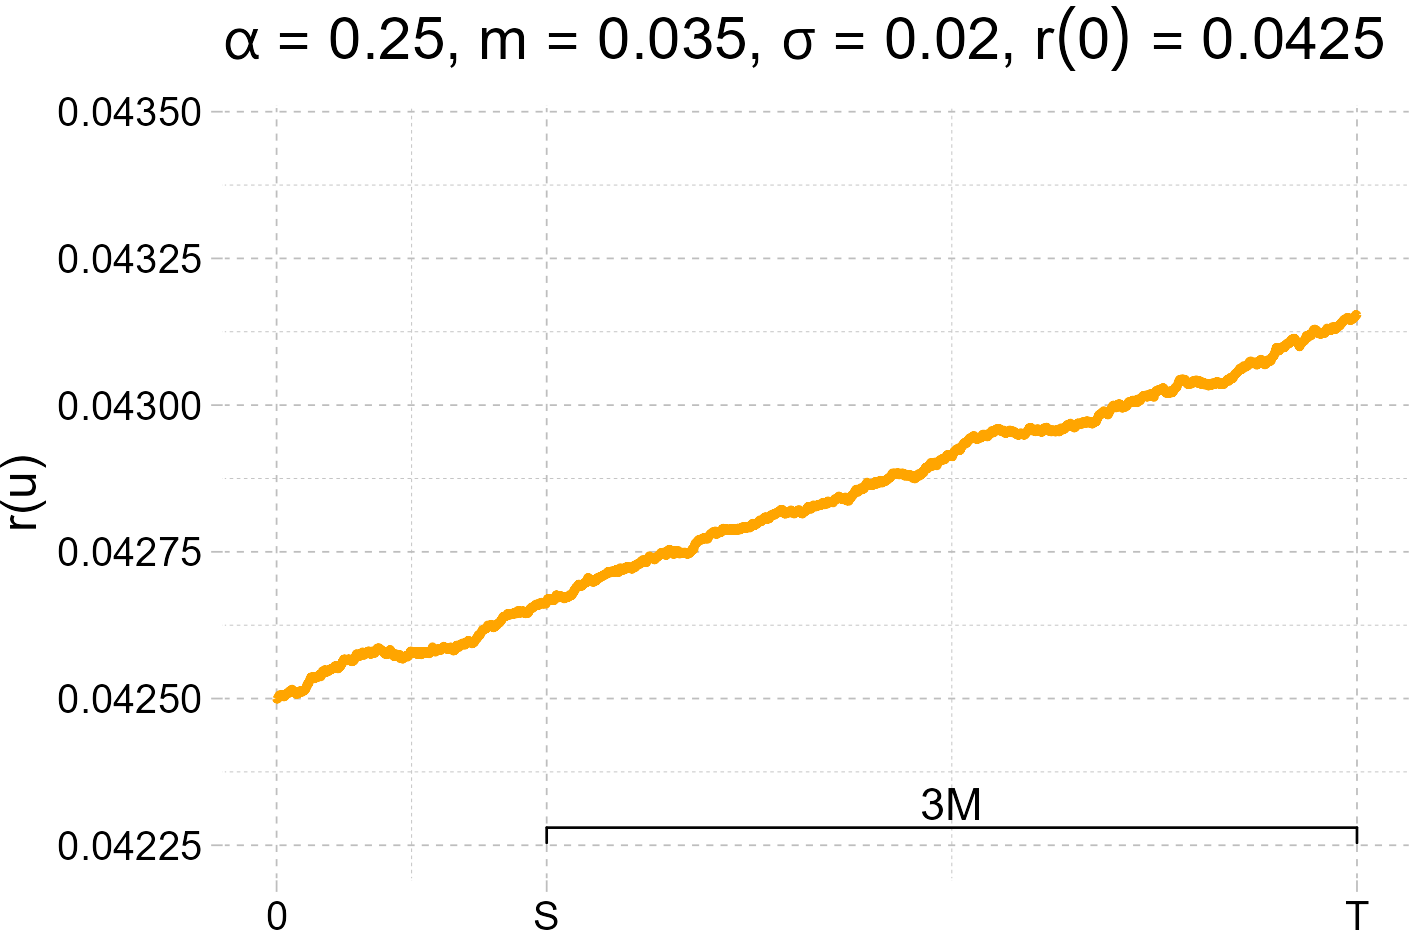
\includegraphics[width=12cm]{figures/SOFR/Vasicek_path.png}
    \caption{Path of Vasicek model for $u\in [0,T]$}
    \label{fig: Vasicek_path}
\end{figure}

\newpage 
\textbf{3M-arithmetic vs $\hat{a}_{0}^{3M}$ 3M-SOFR futures calculations:}
\\~\\
We have that: 
\begin{align*}
\hat{a}_{t}^{3M} = \frac{
\int_{S}^{T}\E_{Q}[r(u)|\F_{t}]du
}{
(T-S)f^{3M}(t,S,T)
}    
\end{align*}

For calculating $f^{3M}(t,S,T)$ we have from 
Equation \ref{eq: Vasicek_3M_SOFR_closed_formula} p.\pageref{eq: Vasicek_3M_SOFR_closed_formula}, that:  
\begin{align*}
f^{3M}(t,S,T) &= 
\frac{1}{T-S}\left[
\exp\left(
A(t,S,T) + B(t,S,T)r(t)
\right)
-1
\right]
\end{align*}

Where: 
\begin{align*}
A(t,S,T) &= m(T-S) - \frac{m}{\alpha}\left[
e^{-\alpha(S-t)} - e^{-\alpha(T-t)}
\right] + \frac{1}{2}\frac{\sigma^{2}}{\alpha^{2}}\int_{t}^{T}\Sigma^{2}(u,t,S,T)du \\
B(t,S,T) &= \frac{1}{\alpha}\left[
e^{-\alpha(S-t)} - e^{-\alpha(T-t)}
\right]
\end{align*}

We are interested in the case where $t=0$, giving us:
\begin{align*}
\hat{a}_{0}^{3M} = \frac{
\int_{S}^{T}\E_{Q}[r(u)]du
}{
(T-S)f^{3M}(0,S,T)
}
= 0.995
\end{align*}

\textbf{3M-arithmetic vs $(\hat{a}_{0}, \hat{b}_{0}, \hat{c}_{0})$ 1M-SOFR futures calculations}
\\~\\
In this simulation we had that Condition \ref{eq: condition_det(M)_not_zero} were met, as we got:
\begin{align*}
\alpha_{0} &= 0.0423 \\ 
\beta_{0} &= 0.0421 \\ 
\gamma_{0} &= 0.0420
\end{align*}

Furthermore, the optimal weight $\hat{\mathbf{x}}_{0}$ turned out to be:
\begin{align*}
\hat{\mathbf{x}}_{0} &= 
\begin{bmatrix}
\alpha_{0}^{2} & \alpha_{0}\beta_{0} & \alpha_{0}\gamma_{0} \\ 
\beta_{0}^{2} & \alpha_{0}\beta_{0} & \beta_{0}\gamma_{0} \\ 
\gamma_{0}^{2} & \alpha_{0}\gamma_{0} & \beta_{0}\gamma_{0}
\end{bmatrix}^{-1}
\begin{bmatrix}
q_{0}\alpha_{0} \\ 
q_{0}\beta_{0} \\ 
q_{0}\gamma_{0}
\end{bmatrix}
=
\begin{bmatrix}
0.501 \\
0.501 \\
-0.004
\end{bmatrix} 
\end{align*}

Here:
\[
q_{0} = \E_{Q}[X^{3M_{A}}(S,T)] = 0.0421
\]


\newpage


\textbf{3M-arithmetic vs 3M-geometric SOFR futures:}

\begin{figure}[htp]
    \centering
    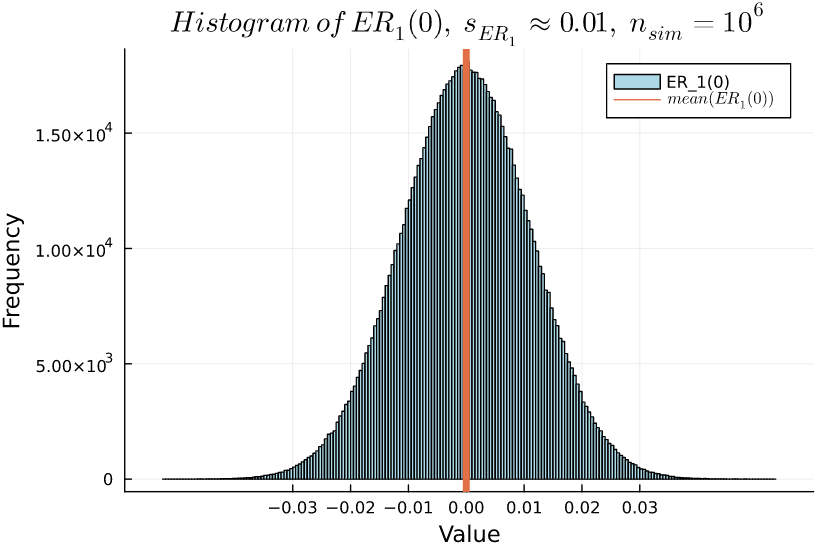
\includegraphics[width=12cm]{figures/SOFR/ER_1(0).PNG}
    \caption{Simulation of $ER_{1}(0)$}
    \label{fig: ER_1_(0)}
\end{figure}

Here we see the distribution $ER_{1}(0)$, we see that the mean of $ER_{1}(0)$, $\overline{ER_{1}(0)} = 0$, this indicates that one average hedging $X^{3M_{A}}(S,T)$ where one takes $\hat{a}_{0} = 0.995$-positions in $3M$-SOFR futures would be a good hedge. We also have that $\E_{Q}[ER_{1}(0)] = 0$.  
\\~\\
\textbf{3M-arithmetic vs $(\hat{a}_{0}, \hat{b}_{0}, \hat{c}_{0})$ 1M-SOFR futures}

\begin{figure}[htp]
    \centering
    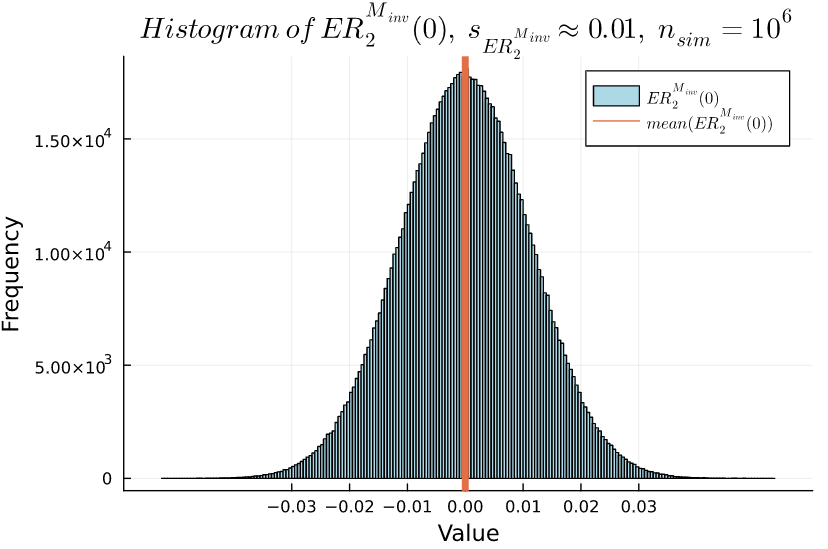
\includegraphics[width=12cm]{figures/SOFR/ER_2(0)_M_inv.PNG}
    \caption{Simulation of $ER_{2}^{inv}(0)$}
    \label{fig: ER_2_(0)_M_inv}
\end{figure}

Here we see the $ER_{2}(0)$ distribution under the assumption that $M$ is invertible. Here we have taken the following position in $1M$-SOFR futures: 
\[
(\hat{a}_{0}, \hat{b}_{0}, \hat{c}_{0})
= 
(0.501, 0.501, -0.004)
\]
We see that the mean of $ER_{2}^{M_{inv}}(0)$, $\overline{ER_{2}^{M_{inv}}(0)} = 0$, which then again indicated that on average taking the above position at time $t=0$ would be a good hedge. 
\\~\\ 



\chapter{ESG swaps}


\section{ESG}
ESG \nomenclature{ESG}{Environmental, Social, and Governance} stands for Environmental, Social, and Governance. ESG metrics are becoming more critical for the financial sector in the European Union. The European Union have established a new taxonomy \cite{EU:2021} for sustainable activities. 
\\~\\
This taxonomy is put in place so that the EU can be carbon neutral by 2050, the goal is to help investors and companies contribute to the Paris Climate agreement. It will enable companies and issuers to access financing consistent with these goals.
\\~\\ 
One such contribution could be to access cheaper swap prices by meeting certain ESG criteria. Which in our case will be a particular ESG score. Let us take a look at what the different letters could represent:
\begin{itemize}
    \item Environmental: typically Climate risks, one metric could be $CO_{2}$-emissions. 
    \item Social: metrics could be: workforce rights, consumer protests etc. 
    \item Governance: management structure, diversity, crisis management, codes of conduct etc. 
\end{itemize}

We will not go into detail when it comes to the ESG risk score, as this would be a thesis in itself. However, we propose a model and show some implications. 

\newpage 

\section{Case study}
Our modelling approach will be based on the ISDA document \cite{ISDA:2021}, and in particular, the interest rate swap between SBM Offshore and ING, where the ESG score is set by Sustainalytics. The deal has the following specifications:
\begin{itemize}
    \item It gets added a positive or negative spread to the fixed rate set at the inception of the swap, based upon SBM's ESG score set by Sustainalytics. 
    \item At the beginning of every year during the life of the swap, ING set's a target ESG score.
    \item If the score has been met, then a discount of 5-10 basis points is applied to the fixed rate.
    \item If the score has not been met, then a penalty of 5-10 basis points is applied to the fixed rate. 
\end{itemize} 

In our simulation we will consider the ESG criteria to be $\F_{0}$-measurable, we will also take a constant discount $d$. To exemplify this deal pretend that the original fixed rate was set at $\kappa = 0.07$, with a discount/penalty $d = 0.005$ and the contract length is $n=4$ years. 
\\~\\
Assume that SBM Offshore met the criteria the first three times but did not meet the criteria the last time, that would given arise to the following ESG fixed rate sequence: 
\begin{align*}
K_{1}^{ESG} &=  0.065, \;\; 
K_{2}^{ESG} =   0.060, \;\;
K_{3}^{ESG} =   0.055, \;\; 
K_{4}^{ESG} =   0.060
\end{align*}


\begin{figure}[htp]
    \centering
    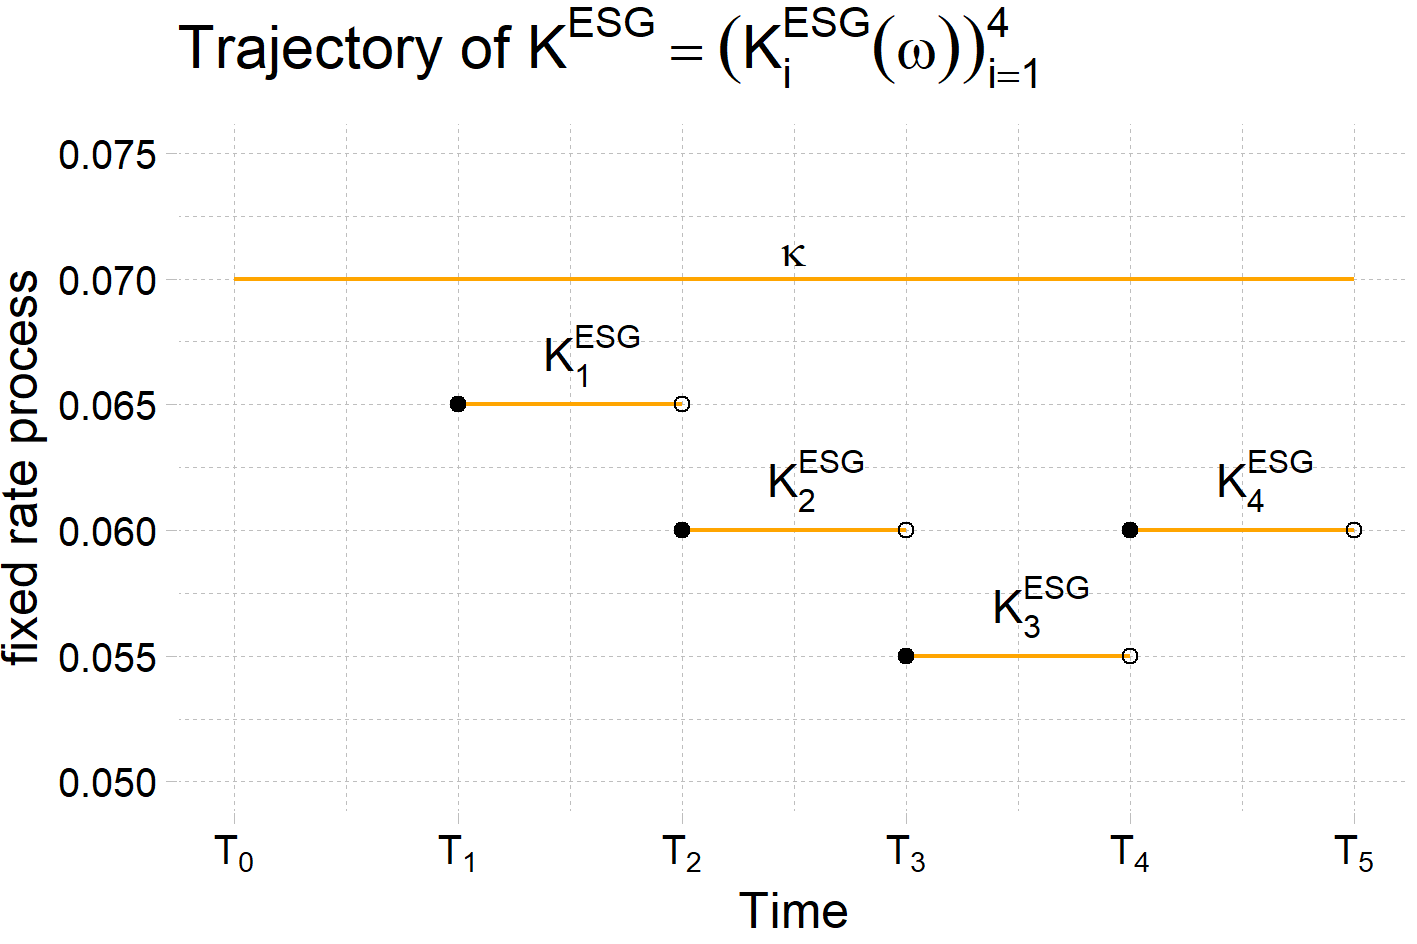
\includegraphics[width=12cm]{figures/ESG/SBM_ESG_path.png}
    \caption{ESG-fixed rate trajectory}
    \label{fig: SBM_ESG_path}
\end{figure}














\newpage 


\section{General setup}
We will take this deal as motivation, but generalize a bit further:
\begin{assumption}
We assume the following: 
\begin{itemize}[leftmargin=*]
    \item $N$ represents the nominal value, think of it as the amount you loan/lend.
    \item $0 < T_{0} < T_{1} < \dots < T_{n}$ a sequence of future dates. 
    \item $\delta = T_{i} - T_{i-1}$ a fixed leg between payments 
    \item $\kappa$ the fixed rate from the original swap, i.e without ESG-link. 
    \item $d$ basis points added or subtracted to the fixed rate $\kappa$
    \item $\{A_{i}\}_{i=1}^{n}$ sequence of events, where: 
    $A_{i} = \{X_{T_{i}} \leq C_{T_{i}}^{ESG}\}$ i.e the sequence of events measuring whether or not the ESG-criteria $C_{T_{i}}^{ESG}$ is met at time $T_{i}$ or not. 
    \item Need to know more about the process $C^{ESG} = (C_{T_{i}}^{ESG})_{i \in \mathcal{I}}$, i.e. is it $\F_{0}$-measurable? or should we say $\F_{t}$-measurable?
\end{itemize}
\end{assumption} 


\begin{definition}[\textbf{ESG fixed rate process}]
Let $K^{ESG} = (K_{i}^{ESG})_{i=1}^{n}$ \nomenclature{$K^{ESG}$}{ESG fixed rate process}
denote the ESG fixed rate process, we define it recursively as: 
\begin{align*}
K_{i}^{ESG}(\omega) &= (K_{i-1}^{ESG}(\omega)-d)\mathbbm{1}_{A_{i}}(\omega)
+ (K_{i-1}^{ESG}(\omega)+d)\mathbbm{1}_{A_{i}^{C}}(\omega), \;\; i\geq 2
\end{align*}

where:
\begin{align*}
K_{1}^{ESG}(\omega) &= (\kappa - d)\mathbbm{1}_{A_{1}}(\omega)
+ (\kappa + d)\mathbbm{1}_{A_{1}^{C}}(\omega)    
\end{align*}
\end{definition} 

\begin{notation}
Let $\mathcal{I} = \{k_{1}, \dots, k_{n}\}$ represent an index set. Furthermore, let\\ 
$k_{1}< \dots < k_{l} < \dots < k_{m}< \dots < k_{n}$ We then define:
\begin{align*}
\left(
\bigcap_{i\in \mathcal{I}}A_{i}
\right)^{
\{(k_{1}, k_{l}, k_{m})\}
}
&= 
A_{k_{1}}^{C}\cap A_{k_{2}} \cap \dots\cap A_{k_{l}}^{C}\cap
A_{k_{l+1}}\cap \dots \cap A_{k_{m}}^{C}\cap A_{k_{m+1}}\cap \dots \cap A_{k_{n}}
\end{align*}
\end{notation}

\begin{result}
\label{prop/result: K_ESG_n}
Let $n \in \N_{2}:= \{k: k\geq 2, k\in \N\}$, consider the above situation. Let $\mathcal{I}_{n} = \{1, \dots, n\}$ and $\mathcal{I}_{2n}^{Even} = \{2, \dots, 2n\}$,
$(A_{i})_{i\in \mathcal{I}}$ denotes the event that the ESG criteria are met.
Let $j_{1} < j_{2} < \dots < j_{|\mathcal{I}_{\alpha}^{Even}|} \in \N$
furthermore $|\mathcal{I}_{2n}^{Even}|$ and $|\mathcal{I}_{n}|$ denotes the cardinality of the respective sets. 
\\~\\ 
We can then express $K_{n}^{ESG}(\omega)$ as:
\begin{align*}
K_{n}^{ESG}(\omega) &= 
[\kappa -dn]\mathbbm{1}\left[
\bigcap_{i\in \mathcal{I}_{n}}A_{i}
\right](\omega) \\ 
&+ 
\sum_{\alpha \in \mathcal{I}_{2n}^{Even}}
\left(
[\kappa -d(n-\alpha)]\mathbbm{1}\left[
\bigcup_{
j_{1}\neq \dots \neq j_{|\mathcal{I}_{\alpha}^{Even}|}
\in \mathcal{I}_{n}
}\left(
\bigcap_{i\in \mathcal{I}_{n}}A_{i}
\right)^{
\{
(j_{1}, \dots , j_{|\mathcal{I}_{\alpha}^{Even}|})
\}
}
\right]
\right)(\omega) 
\end{align*}
\end{result}  


\newpage 

To get a better grasp of Result \ref{prop/result: K_ESG_n}, we include the following graph: 
\begin{figure}[htp]
    \centering
    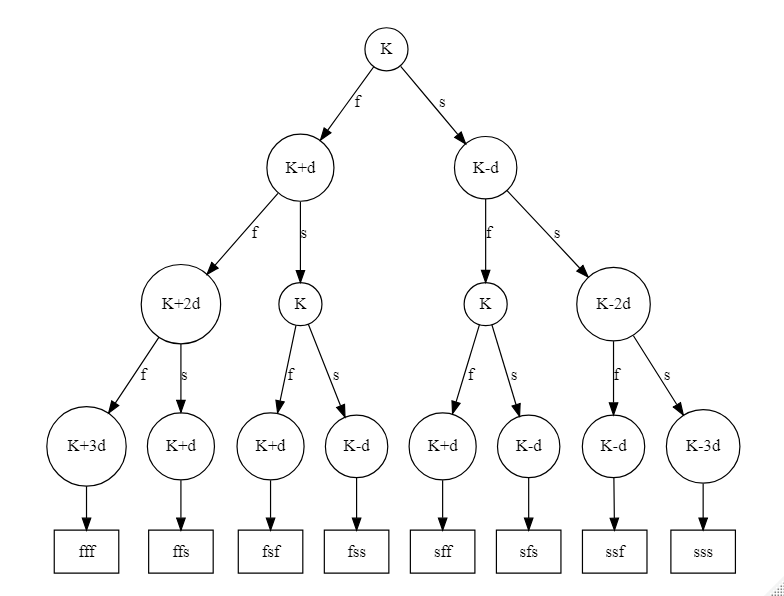
\includegraphics[width=13cm]{figures/ESG/tree_plt_ESG_seq.png}
    \caption{Possible outcomes of $K_{n}^{ESG}(\omega)$}
    \label{fig: Tree_plot_ESG_sequence}
\end{figure}

For a general $n$, we have $2^{n}$ possible paths, and the unique values will be
\begin{align*}
\kappa + id, i\in \{n-2k: k=0, \dots, n\}    
\end{align*}

We will have $|\{n-2k: k=0, \dots, n\}| = n + 1$ unique values. With ${n \choose |i|}$ number of possible paths leading to the value $\kappa + id$. 
\\~\\
Thus for $n = 3$, we have $2^{3} = 8$ possible paths, and $3+1 =4$ unique values: 
\begin{align*}
\kappa +3d, \; \kappa +d,\; \kappa -d\; \kappa - 3d    
\end{align*} 

We see that there are ${3 \choose 1} = 3$ different paths yielding a result of $\kappa +d$, which in this case are: $ffs, fsf$ and $sff$. 

\newpage 

\begin{align*}
K_{3}^{ESG}(\omega) &= 
[\kappa -3d]\mathbbm{1}\left[
\bigcap_{i\in \mathcal{I}_{3}}A_{i}
\right](\omega) \\ 
&+ 
\sum_{\alpha \in \{2,4,6\}}
\left(
[\kappa -d(3-\alpha)]\mathbbm{1}\left[
\bigcup_{\{
j_{1}\neq \dots \neq j_{|\mathcal{I}_{\alpha}^{Even}|}
\}
\in \{1,2,3\}
}\left(
\bigcap_{i =1}^{3}A_{i}
\right)^{
(j_{1}, \dots , j_{|\mathcal{I}_{\alpha}^{Even}|})
}
\right]
\right)(\omega) 
\end{align*}

The number of unique possible outcomes will be $|\{2,4,6\}| + 1 = 4$. If we fix $\alpha$, let's say, $\alpha = 4$, we get the value $\kappa +d$, and there are $3$ paths leading to this result. Now for $j_{1} < j_{2}$, we see that $j_{1} \neq j_{2} \in \{1,2,3\}$, leads to the following set-combinations: 
\begin{align*}
\{1,2\}, \; \{1,3\},\; \{2,3\}    
\end{align*}

Namely $3$ sets, where we got the index of where the criteria were not met. And this corresponds to the following expression: 

\begin{align*}
 &[\kappa - d(3-4)]\mathbbm{1}\left[
\bigcup_{j_{1}\neq j_{2}\in \{1,2,3\}}
\left[\bigcap_{i=1}^{3}A_{i}\right]^{\{(j_{1}, j_{2})\}}
\right](\omega) \\
= &[\kappa + d]\left[
\underbrace{
\mathbbm{1}(A_{1}^{C}\cap A_{2}^{C}\cap A_{3})(\omega)
}_{=ffs}
+ 
\underbrace{
\mathbbm{1}(A_{1}^{C}\cap A_{2}\cap A_{3}^{C})(\omega)
}_{=fsf} + 
\underbrace{
\mathbbm{1}(A_{1}\cap A_{2}^{C}\cap A_{3}^{C})(\omega)
}_{= sff}
\right]   
\end{align*}


\newpage 

\begin{proposition}
\label{prop: cond_expectation_ESG_sequence}
Let us denote $\kappa_{t}^{ESG}(i) := \E_{Q}[K_{i}^{ESG}(\omega)|\F_{t}]$. We then have\\ 
that for $t\leq T_{0}$ that: 
\begin{align*}
\kappa_{t}^{ESG}(i)
&= 
\kappa -d\cdot D(i)
\end{align*}

Where: 
\begin{align*}
 D(i) &= 
i\cdot \E_{Q}\left[
\prod_{l=1}^{i}\mathbbm{1}(A_{l})\bigg{|}\F_{t}
\right]
+ 
\sum_{\alpha \in \mathcal{I}_{2i}^{Even}}[i-\alpha]
\sum_{
j_{1}\neq \dots \neq j_{|\mathcal{I}_{\alpha}^{Even}|}
}
\E_{Q}\left[
\left(
\prod_{l=1}^{i}\mathbbm{1}(A_{l})
\right)^{
\{
(j_{1}, \dots , j_{|\mathcal{I}_{\alpha}^{Even}|})
\}
}
\bigg{|}\F_{t}
\right]   
\end{align*}
\end{proposition}

\begin{proof}

$K_{i}^{ESG}(\omega)$ is as described in Result \ref{prop/result: K_ESG_n}: 

\begin{align*}
\E_{Q}\left[K_{i}^{ESG}(\omega)
\bigg{|}\F_{t}\right]
&= 
[\kappa - d\cdot i]\E_{Q}\left[
\mathbbm{1}\left(
\bigcap_{l=1}^{i}A_{l}
\right)(\omega)\bigg{|}\F_{t}
\right] \\ 
&+
\sum_{\alpha \in \mathcal{I}_{2i}^{Even}}
\left(
[\kappa - d(i-\alpha)]
\E_{Q}\left[
\mathbbm{1}\left[
\bigcup_{\{
j_{1}\neq \dots \neq j_{|\mathcal{I}_{\alpha}^{Even}|}
\}
}
\left(
\bigcap_{l=1}^{i}
A_{l}
\right)
^{
\{
(j_{1}, \dots , j_{|\mathcal{I}_{\alpha}^{Even}|})
\}
}
\right](\omega)
\bigg{|}\F_{t}
\right]
\right)
\end{align*}

Now: 
\begin{align*}
&\E_{Q}\left[
\mathbbm{1}\left[
\bigcup_{\{
j_{1}\neq \dots \neq j_{|\mathcal{I}_{\alpha}^{Even}|}
\}
}
\left(
\bigcap_{l=1}^{i}
A_{l}
\right)^{
\{
(j_{1}, \dots , j_{|\mathcal{I}_{\alpha}^{Even}|})
\}
}
\right](\omega)
\bigg{|}\F_{t}
\right] \\
= 
\sum_{
j_{1}\neq \dots \neq j_{|\mathcal{I}_{\alpha}^{Even}|}
}
&\E_{Q}\left[
\mathbbm{1}\left(
\bigcap_{l=1}^{i}A_{l}
\right)^{
\{
(j_{1}, \dots, j_{|\mathcal{I}_{\alpha}^{Even}|})
\}
}
(\omega)
\bigg{|}\F_{t}
\right]
\end{align*}

Furthermore: 
\begin{align*}
\E_{Q}\left[
\mathbbm{1}\left(
\bigcap_{l=1}^{i}A_{l}
\right)(\omega)\bigg{|}\F_{t}
\right] 
&= \underbrace{
\E_{Q}\left[
\prod_{l=1}^{i}\mathbbm{1}(A_{l})\bigg{|}\F_{t}
\right]
}_{= s(l=1, i)}
\end{align*}

and:
\begin{align*}
\E_{Q}\left[
\mathbbm{1}\left(
\bigcap_{l=1}^{i}A_{l}
\right)^{
\{
(j_{1}, \dots, j_{|\mathcal{I}_{\alpha}^{Even}|})
\}
}(\omega)
\bigg{|}\F_{t}
\right] 
&= \underbrace{
\E_{Q}\left[
\left(
\prod_{l=1}^{i}\mathbbm{1}(A_{l})
\right)^{
\{
(j_{1}, \dots, j_{|\mathcal{I}_{\alpha}^{Even}|})
\}
}
(\omega)
\bigg{|}\F_{t}
\right]
}_{= f(l=1, i, j_{|\mathcal{I}_{\alpha}|})}
\end{align*}

\begin{align*}
\E_{Q}[K_{i}^{ESG}(\omega)|\F_{t}]
&= 
[\kappa -d\cdot i]s(l=1,i) \\
&+ 
\kappa \sum_{\alpha \in \mathcal{I}_{2i}^{Even}}
\sum_{
j_{1}\neq \dots \neq j_{|\mathcal{I}_{\alpha}^{Even}|}
}
f(l=1, i, j_{|\mathcal{I}_{\alpha}^{Even}|}) \\ 
&-
d\sum_{\alpha \in \mathcal{I}_{2i}^{Even}}
[i-\alpha]\sum_{
j_{1}\neq \dots \neq j_{|\mathcal{I}_{\alpha}^{Even}|}
}
f(l=1, i, j_{|\mathcal{I}_{\alpha}^{Even}|})
\end{align*}

\newpage 

We collect $\kappa$ and $d$-terms:
\begin{align*}
\E_{Q}[K_{i}^{ESG}(\omega)|\F_{t}]
&= 
\kappa
\underbrace{
\left[
s(l=1,i) + \sum_{\alpha \in \mathcal{I}_{2i}^{Even}}\sum_{
j_{1}\neq \dots \neq j_{|\mathcal{I}_{\alpha}^{Even}|}
}
f(l=1, i, j_{|\mathcal{I}_{\alpha}^{Even}|}) 
\right]
}_{=M(i)}
\\ 
&-d
\underbrace{
\left[
i\cdot s(l=1,i) + \sum_{\alpha \in \mathcal{I}_{2i}^{Even}}
\left(
[i-\alpha]\sum_{
j_{1}\neq \dots \neq j_{|\mathcal{I}_{\alpha}^{Even}|}
}
f(l=1, i, j_{|\mathcal{I}_{\alpha}^{Even}|})
\right)
\right]
}_{=D(i)} \\ 
&= 
\kappa M(i) -d\cdot D(i)
\end{align*}

Where: 
\begin{align*}
D(i) &= 
i\cdot \E_{Q}\left[
\prod_{l=1}^{i}\mathbbm{1}(A_{l})\bigg{|}\F_{t}
\right]
+ 
\sum_{\alpha \in \mathcal{I}_{2i}^{Even}}[i-\alpha]
\sum_{
j_{1}\neq \dots \neq j_{|\mathcal{I}_{\alpha}^{Even}|}
}
\E_{Q}\left[
\left(
\prod_{l=1}^{i}\mathbbm{1}(A_{l})
\right)^{
\{
(j_{1}, \dots , j_{|\mathcal{I}_{\alpha}^{Even}|})
\}
}
\bigg{|}\F_{t}
\right]
\end{align*}

and: 
\begin{align*}
M(i) &= 
\E_{Q}\left[
\prod_{l=1}^{i}\mathbbm{1}(A_{l})\bigg{|}\F_{t}
\right]  
+\sum_{\alpha \in \mathcal{I}_{2i}^{Even}}
\sum_{
j_{1}\neq \dots \neq j_{|\mathcal{I}_{\alpha}^{Even}|}
}
\E_{Q}\left[
\left(
\prod_{l=1}^{i}\mathbbm{1}(A_{l})
\right)^{
\{
(j_{1}, \dots , j_{|\mathcal{I}_{\alpha}^{Even}|})
\}
}
\bigg{|}\F_{t}
\right]
\end{align*}

Let's rewrite $M(i)$ on set notation again: 
\begin{align*}
M(i) &= 
\E_{Q}\left[
\mathbbm{1}\left(
\bigcap_{l \in \mathcal{I}_{i}}A_{l}
\right)
\bigg{|}\F_{t}
\right]
+\sum_{\alpha \in \mathcal{I}_{2i}^{Even}}
\E_{Q}\left[
\mathbbm{1}
\left[
\bigcup_{
j_{1} \neq \dots \neq j_{|\mathcal{I}_{\alpha}^{Even}|}
}
\left(
\bigcap_{l \in \mathcal{I}_{i}}A_{l}
\right)^{
\{
(j_{1}, \dots, j_{|\mathcal{I}_{\alpha}^{Even}|})
\}
}
\right]
\bigg{|}\F_{t}
\right]
\end{align*}

For $i = 1, \dots, n$, we have: 
\begin{align*}
\Omega_{i} 
&= 
\underbrace{
\left[
\sum_{\alpha \in \mathcal{I}_{2i}^{Even}}
\bigcup_{
j_{1} \neq \dots \neq j_{|\mathcal{I}_{\alpha}^{Even}|}
}
\left(
\bigcap_{l \in \mathcal{I}_{i}}A_{l}
\right)^{
\{
(j_{1}, \dots, j_{|\mathcal{I}_{\alpha}^{Even}|})
\}
}
\right]
}_{=\mathcal{H}_{i}}
\bigcup
\underbrace{
\left[
\bigcap_{l \in \mathcal{I}_{i}}A_{l}
\right]
}_{=\mathcal{L}_{i}}
\;\; 
\text{with}\;\; 
Q(\Omega_{i}) = 1
\end{align*} 

Now as $\mathcal{H}_{i}\cap \mathcal{L}_{i} = \emptyset$, 
and $\mathcal{H}_{i}\cup \mathcal{L}_{i} = \Omega_{i}$, in addition to exploiting the linearity of the expectation operator we get:

\begin{align*}
M(i) 
&= 
\E_{Q}\left[
\mathbbm{1}\left[
\left[
\sum_{\alpha \in \mathcal{I}_{2i}^{Even}}
\bigcup_{
j_{1} \neq \dots \neq j_{|\mathcal{I}_{\alpha}^{Even}|}
}
\left(
\bigcap_{l \in \mathcal{I}_{i}}A_{l}
\right)^{
\{
(j_{1}, \dots, j_{|\mathcal{I}_{\alpha}^{Even}|})
\}
}
\right]
\bigcup
\left[
\bigcap_{l \in \mathcal{I}_{i}}A_{l}
\right]
\right]
\bigg{|}\F_{t}
\right] \\ 
&= 
\E_{Q}\left[
\mathbbm{1}(\Omega_{i})|\F_{t}
\right] \\ 
&= 
1
\end{align*}

Leaving us with: 
\begin{align*}
\E_{Q}[K_{i}^{ESG}(\omega)|\F_{t}] &= 
\kappa - d\cdot D(i) := \kappa_{t}^{ESG}(i)
\end{align*}


\end{proof}


\section{Zero Coupon Bond ESG-swap}

\begin{proposition}
Consider a zero coupon bond swap, i.e where the situation is as described in Section \cref{sec: ZCB_swap}, we then get that the
\\ 
ESG-swap rate process $\kappa^{ESG}_{t} = (\kappa_{t}^{ESG}(i))_{i=1, \dots, n}$ is given by: 
\begin{align*}
\kappa_{t}^{ESG}(i) &= \kappa_{t}^{ZCB} -d\cdot D(i)    
\end{align*}
Where: 
\begin{align*}
\kappa_{t}^{ZCB} &=  
\frac{
P(t,T_{0}) - P(t,T_{n})
}{
\delta\sum_{i=1}^{n}P(t,T_{i})
}
\end{align*}
And $D(i)$ is as described in Proposition \ref{prop: cond_expectation_ESG_sequence}

\end{proposition}

\begin{proof}
Now from Section \cref{sec: ZCB_swap} we have that: 
\begin{align*}
\kappa_{t}^{ZCB} &=  
\frac{
P(t,T_{0}) - P(t,T_{n})
}{
\delta\sum_{i=1}^{n}P(t,T_{i})
}    
\end{align*}

Thus: 
\begin{align*}
\kappa_{t}^{ESG}(i) &= \kappa_{t}^{ZCB} -d\cdot D(i)    
\end{align*}
\end{proof}


\newpage 

\section{ESG-swap with SOFR-futures as floating}

\begin{proposition}
The fixed swap rate $\kappa_{t}^{kM-SOFR}$ in a swap with 1M/3M-SOFR as floating is given by:  
\begin{align*}
 \kappa_{t}^{kM-SOFR} &= 
 \frac{
 \sum_{i=1}^{n}P(t,T_{i})f^{kM}(t,T_{i-1}, T_{i})
 }{
 \sum_{i=1}^{n}P(t,T_{i})
 }, \;\; k = 1,3
\end{align*}
\end{proposition}

\begin{proof}
    
In this swap, we have the following specification, at time $T_{i}$:
\begin{itemize}[leftmargin=*]
    \item Pay $\kappa_{t}^{kM-SOFR}\delta N$ (-)
    \item Receive $f^{kM}(t,T_{i-1}, T_{i})\delta N$, \; k=1,3 (+)
\end{itemize} 

\textbf{Cash flow at time $T_{i}$}:
\begin{align*}
f^{kM}(t, T_{i-1}, T_{i})\delta N - \kappa_{t}^{kM-SOFR}\delta N =
[f^{kM}(t,T_{i-1}, T_{i}) -\kappa_{t}^{kM-SOFR}]\delta N, \;\; k=1,3
\end{align*}

\textbf{Time $t$-value for $t\leq T_{0}$ at time $T_{i}$}: 
\begin{align*}
P(t,T_{i})[f^{kM}(t,T_{i-1}, T_{i}) - \kappa_{t}^{SOFR}]\delta N,\;\; k=1,3
\end{align*}

\textbf{Total payer cash flow:}
\begin{align*}
\mathcal{C}_{P}^{kM-SOFR}(t) &= 
\delta N \sum_{i=1}^{n}P(t,T_{i})[f^{kM}(t,T_{i-1}, T_{i}) - \kappa_{t}^{kM-SOFR}], \;\; k=1,3
\end{align*} 

$\kappa_{t}^{kM-SOFR}$ should be chosen such that: 
\begin{align*}
\E_{Q}[\mathcal{C}_{P}^{kM-SOFR}(t)|\F_{t}] = 0    
\end{align*}

Thus: 
\begin{align*}
\sum_{i=1}^{n}P(t,T_{i})f^{kM}(t,T_{i-1}, T_{i}) &= \sum_{i=1}^{n}P(t,T_{i})\kappa_{t}^{kM-SOFR} \\ 
&\Downarrow \\ 
\kappa_{t}^{kM-SOFR} &= \frac{
\sum_{i=1}^{n}P(t,T_{i})f^{kM}(t,T_{i-1}, T_{i})
}{
\sum_{i=1}^{n}P(t,T_{i})
}
\end{align*}
\end{proof}

\chapter{Numerical Simulation}

\section{Introduction}

Assume that we can model the \textbf{ESG-index} as: 
\[
X(t) = 100\exp(-Z(t))
\]

Where $Z(t)$ is an OU-process given by: 
\begin{align*}
dZ(t) &= -\beta Z(t)dt + dI(t)    
\end{align*} 
and: 
\begin{align*}
I(t) &= \sum_{k=1}^{N(t)}J_{k}, \;\; J_{k}\sim Exp(\mu),\;\; N(t) \sim Pois(\lambda t)    
\end{align*} 

For $J\sim Exp(\mu)$, we have:
\begin{align*}
f_{J}(x) &= \mu e^{-\mu x}\mathbbm{1}_{[0,\infty)}(x), \;\; 
\E[J] = \frac{1}{\mu}, \;\text{and}\; Var[J] = \frac{1}{\mu^{2}}
\end{align*}

An explicit solution is given by: 
\begin{align}
\label{eq: characteristic_function_Z(t)}
d[e^{\beta t}Z(t)] &= d[e^{\beta t}]Z(t) + e^{\beta t}dZ(t) \nonumber \\ 
&= \beta e^{\beta t}Z(t)dt + e^{\beta t}[-\beta Z(t)dt + dI(t)]
\nonumber \\ 
&= e^{\beta t}dI(t) \nonumber \\ 
&\Downarrow \nonumber\\ 
Z(t) &= Z(0)e^{-\beta t} + \int_{0}^{t}e^{-\beta (t-s)}dI(s)
\end{align} 


We can also control the limiting distribution of $Z$, by Theorem (\textbf{SATO 1999, thm 17, find this reference later}) 

\newpage 

\begin{proposition}
\begin{align*}
\E\left[
\exp(iu Z(t))
\right] 
&= 
\exp\left(
iuZ(0)e^{-\beta t}\right)
\left(
\frac{
1-iue^{-\beta t}1/\mu}
{
1-iu1/\mu
}
\right)^{\frac{\lambda}{\beta}}
\end{align*}
\end{proposition}

\begin{proof}
Now the characteristic function of Equation \ref{eq: characteristic_function_Z(t)}, is given by: 
\begin{align*}
\E\left[
\exp(iu Z(t))
\right] 
&= 
\exp\left(
iuZ(0)e^{-\beta t}\right) 
\E\left[
\exp\left(iu\int_{0}^{t}e^{-\beta(t-s)}dI(s)\right)
\right]
\end{align*}

Furthermore from Proposition \ref{prop: Integral_g(s)dI(s)}, we have: 
\begin{align*}
\E\left[
\exp\left(iu\int_{0}^{t}e^{-\beta(t-s)}dI(s)\right)
\right] 
&= 
\exp\left(
\int_{0}^{t}\Psi(ue^{-\beta s})ds
\right)
\end{align*}

To ease some notation, we write:
\begin{align*}
\Psi(x) &= \lambda(\varphi_{F}(x) - 1), \;\text{where:}\; 
\varphi_{F}(x) = \int_{\R}e^{iyx}F_{J}(dy) 
\end{align*}

We start with calculating $\varphi_{F}(x)$ with $F_{J}(dy) = 
\mu e^{-\mu y}\mathbbm{1}_{[0,\infty)}(y)dy:$ 
\begin{align*}
\varphi_{F}(x) &= 
\int_{0}^{\infty}e^{ixy}\mu e^{-\mu y}dy   
= \frac{1}{1-ix\frac{1}{\mu}}
\end{align*}

Giving us:
\begin{align*}
\varphi_{F}(x) - 1
= 
\frac{1}{1-ix\frac{1}{\mu}} - \frac{1-ix\frac{1}{\mu}}{1-ix\frac{1}{\mu}} 
= 
\frac{ix\frac{1}{\mu}}{1-ix\frac{1}{\mu}}
\end{align*}

Now: 
\begin{align*}
\Psi(ue^{-\beta s}) &= \lambda(\varphi_{F}(ue^{-\beta s})) -1) \\ 
&= \lambda\left(
\frac{iue^{-\beta s}1/\mu}{1-iue^{\beta s}1/\mu}
\right)\cdot \frac{\beta}{\beta} \\ 
&= 
\frac{\lambda}{\beta}\left(
\frac{\beta iue^{-\beta s}1/\mu}{1-iue^{\beta s}1/\mu}
\right)
\end{align*}

We observe: 
\begin{align*}
h(s) :&= \ln[1-iue^{-\beta s}1/\mu] \\ 
&\Downarrow \\ 
h'(s) &= \frac{\beta iue^{-\beta s}1/\mu}{1-iue^{\beta s}1/\mu} 
\end{align*}

Leaving us with: 
\begin{align*}
\int_{0}^{t}\Psi(ue^{-\beta s})ds
&= 
\frac{\lambda}{\beta}\int_{0}^{t}h'(s)ds
= 
\frac{\lambda}{\beta}[h(t)-h(0)] 
= 
\frac{\lambda}{\beta}
\ln\left[
\frac{1-iue^{-\beta t}1/\mu}{1-iu1/\mu}
\right]
\end{align*}

Thus:
\begin{align*}
\E\left[
\exp(iu Z(t))
\right] 
&= 
\exp\left(
iuZ(0)e^{-\beta t}\right)
\left(
\frac{
1-iue^{-\beta t}1/\mu}
{
1-iu1/\mu
}
\right)^{\frac{\lambda}{\beta}}
\end{align*}
\end{proof}

We can only control the asymptotic distribution of $X$, now if $\beta > 0$, then:  
\begin{align*}
\varphi_{Z_{\infty}}(u) &= 
\frac{\lambda}{\beta}
\int_{0}^{\infty} 
\frac{
\beta iu\eta e^{\beta s}\frac{1}{\mu}
}{
1-iu\eta e^{-\beta s} \frac{1}{\mu}
}ds \\ 
&= 
\exp\left(
\frac{\lambda}{\beta}\ln\left[
1- i\frac{1}{\mu}u\eta e^{-\beta s}
\right]\bigg{|}_{0}^{\infty}
\right) \\ 
&= 
\exp\left(
-\frac{\lambda}{\beta}\ln(1-i\frac{1}{\mu}u\eta)
\right) \\ 
&= 
\frac{1}{
(1-i\frac{1}{\mu}u\eta)^{\frac{\lambda}{\beta}}
}
\end{align*}

Here we use that if $M \sim \Gamma(a,b)$, then: 
\begin{align*}
f_{M}(x;a,b) &= \frac{1}{b^{a}\Gamma(a)}x^{a-1}e^{-\frac{x}{b}}\mathbbm{1}(x>0)\;\text{and}\; 
\varphi_{M}(u) = (1-biu)^{-a}
\end{align*}

We have that: 
\begin{align*}
\varphi_{Z_{\infty}}(u) &= 
\frac{1}{
(1-i\frac{1}{\mu}u\eta)^{\frac{\lambda}{\beta}}
}
= 
\left(
1 - \frac{\eta}{\mu}iu
\right)^{-\frac{\lambda}{\beta}}
\end{align*}

Meaning that
\[
Z_{\infty} \sim \Gamma\left(
\frac{\lambda}{\beta}, \frac{\eta}{\mu}
\right)
\]

Thus if one for instance have $\lambda = 10, \beta = 1, \eta = 1$ and $\mu = \frac{1}{2}$, giving us $a = 10$ and $b= 2$, then the density of $Z_{\infty}\sim \Gamma(10,2)$ would look like:

\begin{figure}[htp]
    \centering
    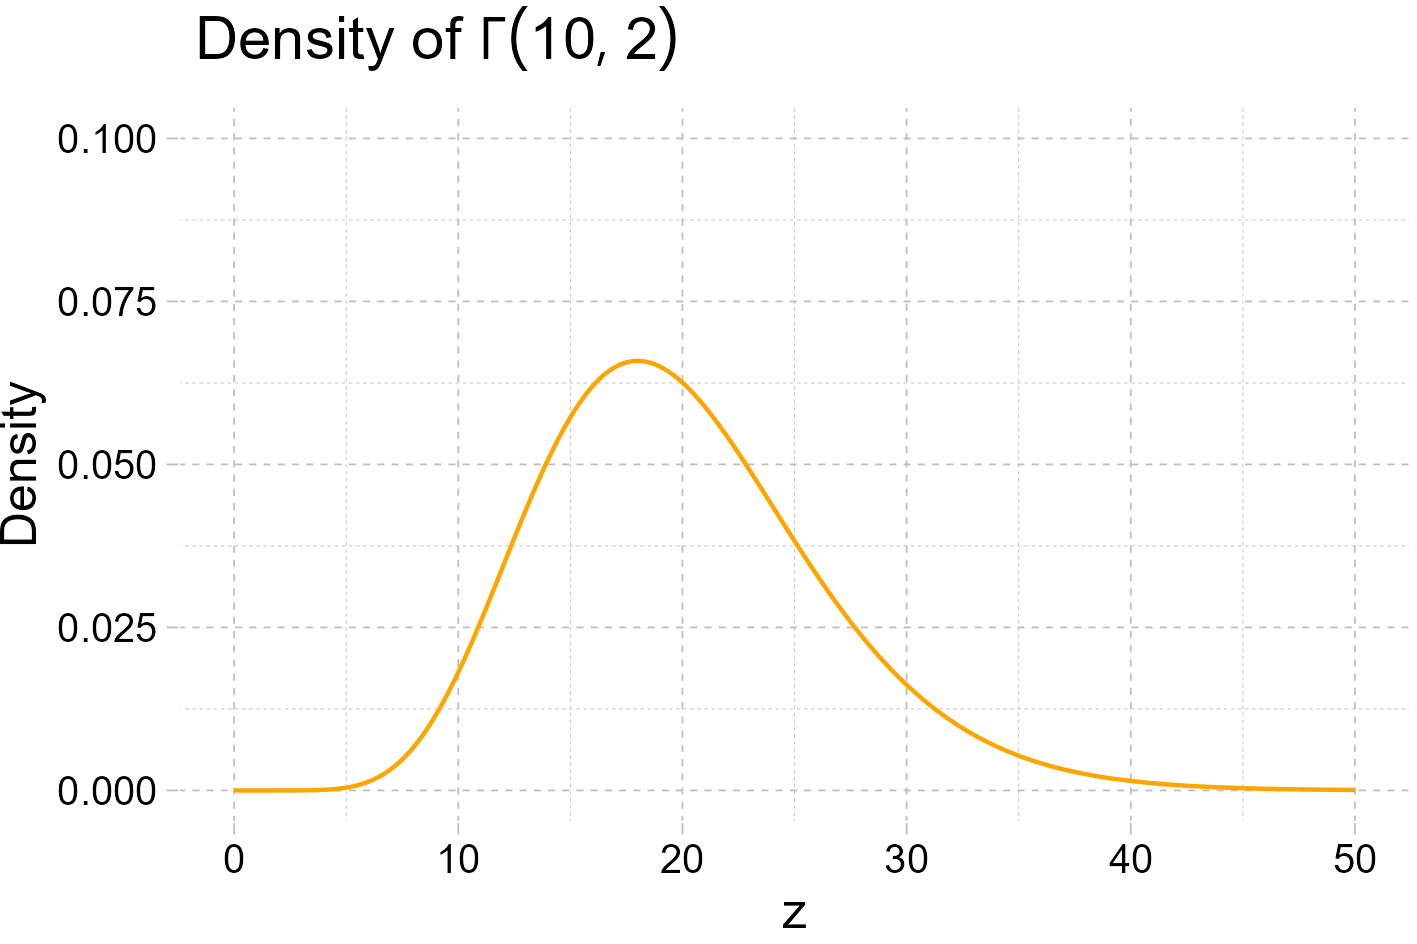
\includegraphics[width=10cm]{figures/ESG/gamma_limiting_dist.png}
    \caption{Distribution of $\Gamma(10, 2)$}
    \label{fig: gamma_limiting_dist}
\end{figure}

\newpage 

\section{Simulation of Zero Coupon Bond ESG-swap}

\textbf{Agreement}: 
\begin{itemize}[leftmargin =*]
    \item We agree upon $C^{ESG} = (C_{T_{i}}^{ESG})_{i\in \{1,2,3,4\}} = (17.6, 16.6, 15.6, 14.55)$ 
    \item One evaluates the ESG-risk score at $(T_{1}, T_{2}, T_{3}, T_{4}) = (1.25, 2.25, 3.25, 4.25)$
\end{itemize}

\textbf{Parameters}:
\begin{itemize}
    \item $d = 0.005$
    \item $\delta = 1$
    \begin{align*}
    \left(
    Z(0) = -\ln(\frac{20}{100}), \beta = -0.05, \lambda = 20, \mu = 150, \Delta t = \frac{1}{360}
    \right)   
\end{align*} 
    \item \begin{align*}
        \left(
        P(t,T_{0}) = 0.995, P(t,T_{1}) = 0.985, P(t,T_{3}) = 0.975, P(t,T_{4}) = 0.965
        \right)
    \end{align*}
    \item Number of simulations: $10^{6}$
\end{itemize}

We assume that the dynamics under $Q$ look the following: 
\begin{figure}[htp]
    \centering
    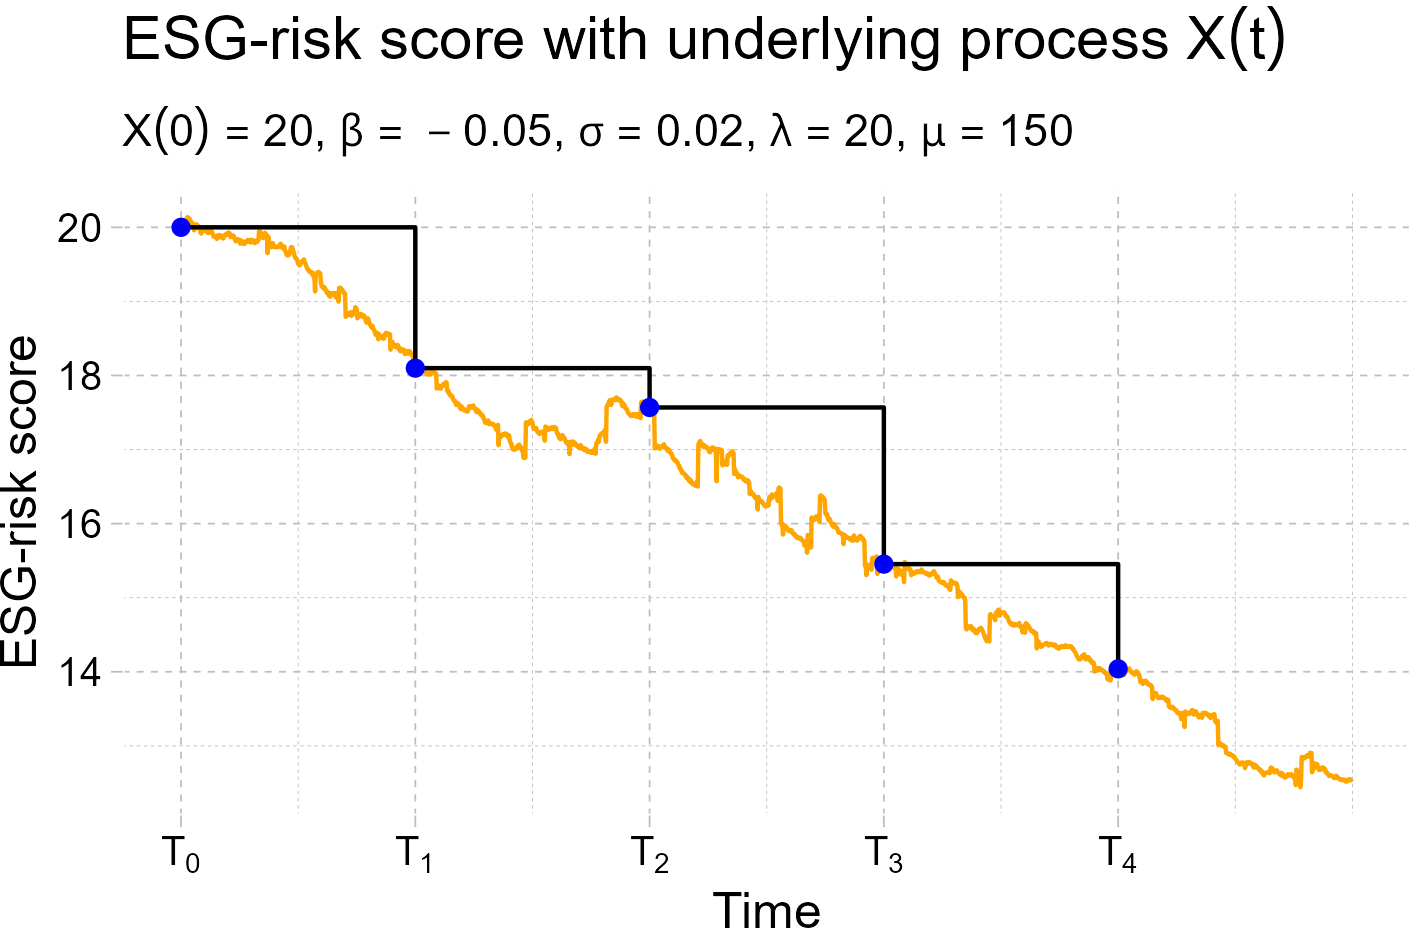
\includegraphics[width=10cm]{figures/ESG/ESG_OU_path.png}
    \caption{trajectory of $X(t)$}
    \label{fig: ESG-risk score}
\end{figure}

This graph indicates that the ESG-risk score is downward trending, this could be that the company are/will implement measures to reduce $CO_{2}$-emissions.
The blue dots represent the ESG-risk score at times $T_{i}$. 


\newpage 

In this simulation we got: 
\begin{align*}
\kappa_{t}^{ZCB} &= \frac{P(t,T_{0})-P(t,T_{4})}{\delta \sum_{i=1}^{4}P(t,T_{i})} = 0.01030   
\end{align*}

\begin{figure}[htp]
    \centering
    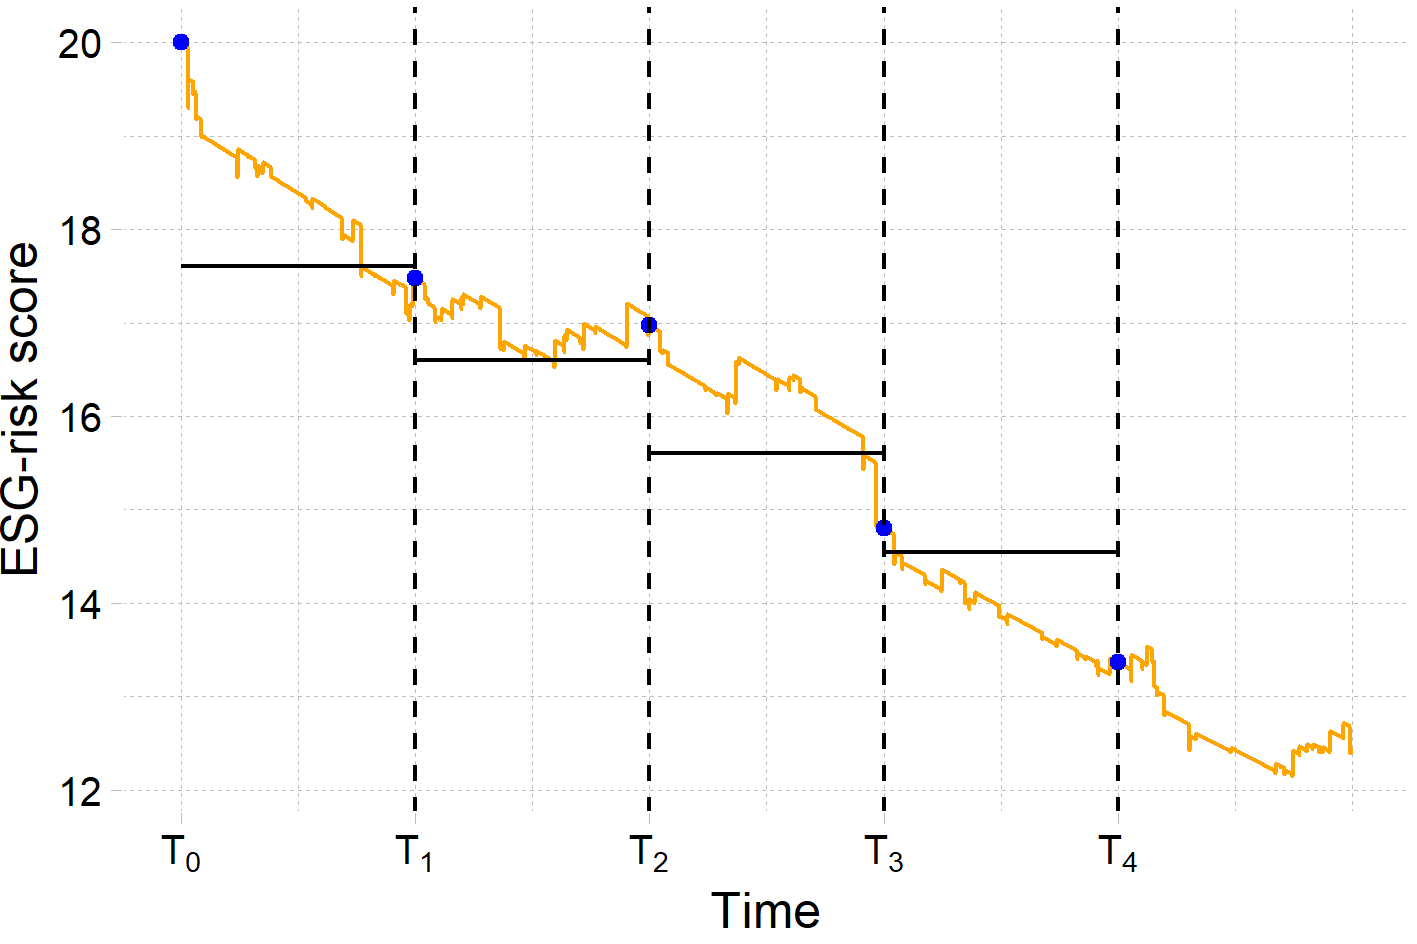
\includegraphics[width= 9cm]{figures/ESG/ESG_plt_criteria.png}
    \caption{ESG-risk score where ESG-criteria is reasonable}
    \label{fig: ESG-risk_criteria1}
\end{figure}

In this figure, we see the underlying ESG risk score process. Here the dark-solid lines represent the criteria $C_{T_{i}}^{ESG}$. We see that the ESG criteria were bearly met at time $T_{1}$, it was not met at $T_{2}$, met at $T_{3}$ and then met again at time $T_{4}$. 
\\~\\ 
We summarize the findings in the following table:
\begin{center}
    \begin{tabular}{ | l | l | l | p{5cm} |}
    \hline
    Time    &   Criteria  & $\kappa_{t}^{ESG}(i)$ \\ \hline
    $T_{1}$ &      17.6   & $0.01224$  \\ \hline
    $T_{2}$ &      16.6   & $0.01119$  \\ \hline
    $T_{3}$ &      15.6   & $0.01023$  \\ \hline
    $T_{4}$ &      14.55  & $0.00780$   \\ \hline
    \end{tabular}
\end{center} 

\begin{figure}[htp]
    \centering
    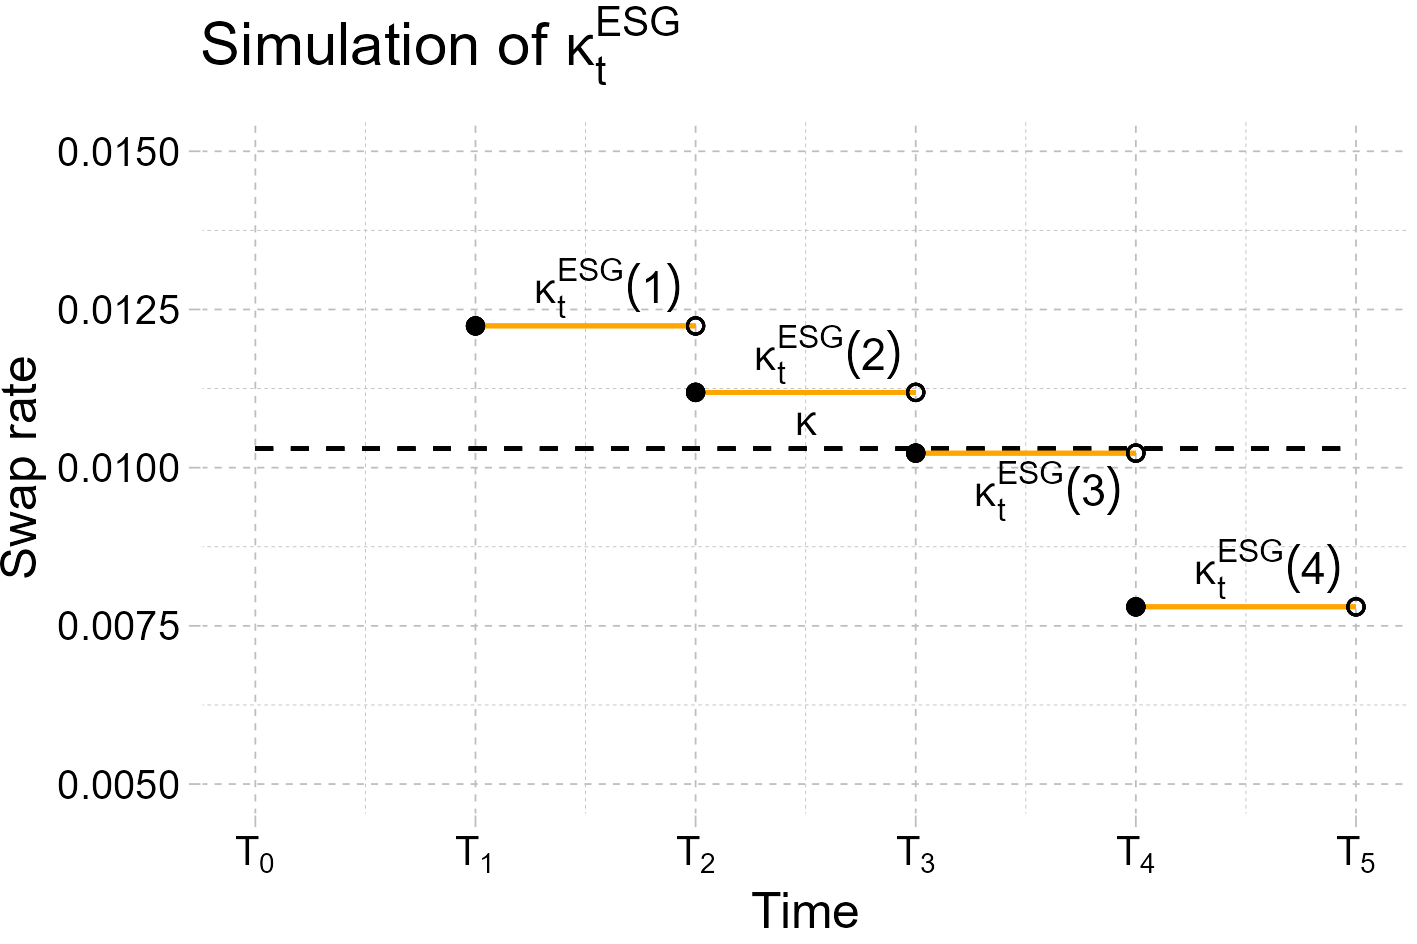
\includegraphics[width= 10cm]{figures/ESG/kappa_t_ESG_1.png}
    \caption{ESG-risk score where ESG-criteria is reasonable}
    \label{fig: ESG_swap_1}
\end{figure}

\newpage 

\textbf{Meeting criteria often}
\\~\\ 
In this simulation we took: $C^{ESG} = (18,17,16,15)$, and we got the following: 

\begin{figure}[htp]
    \centering
    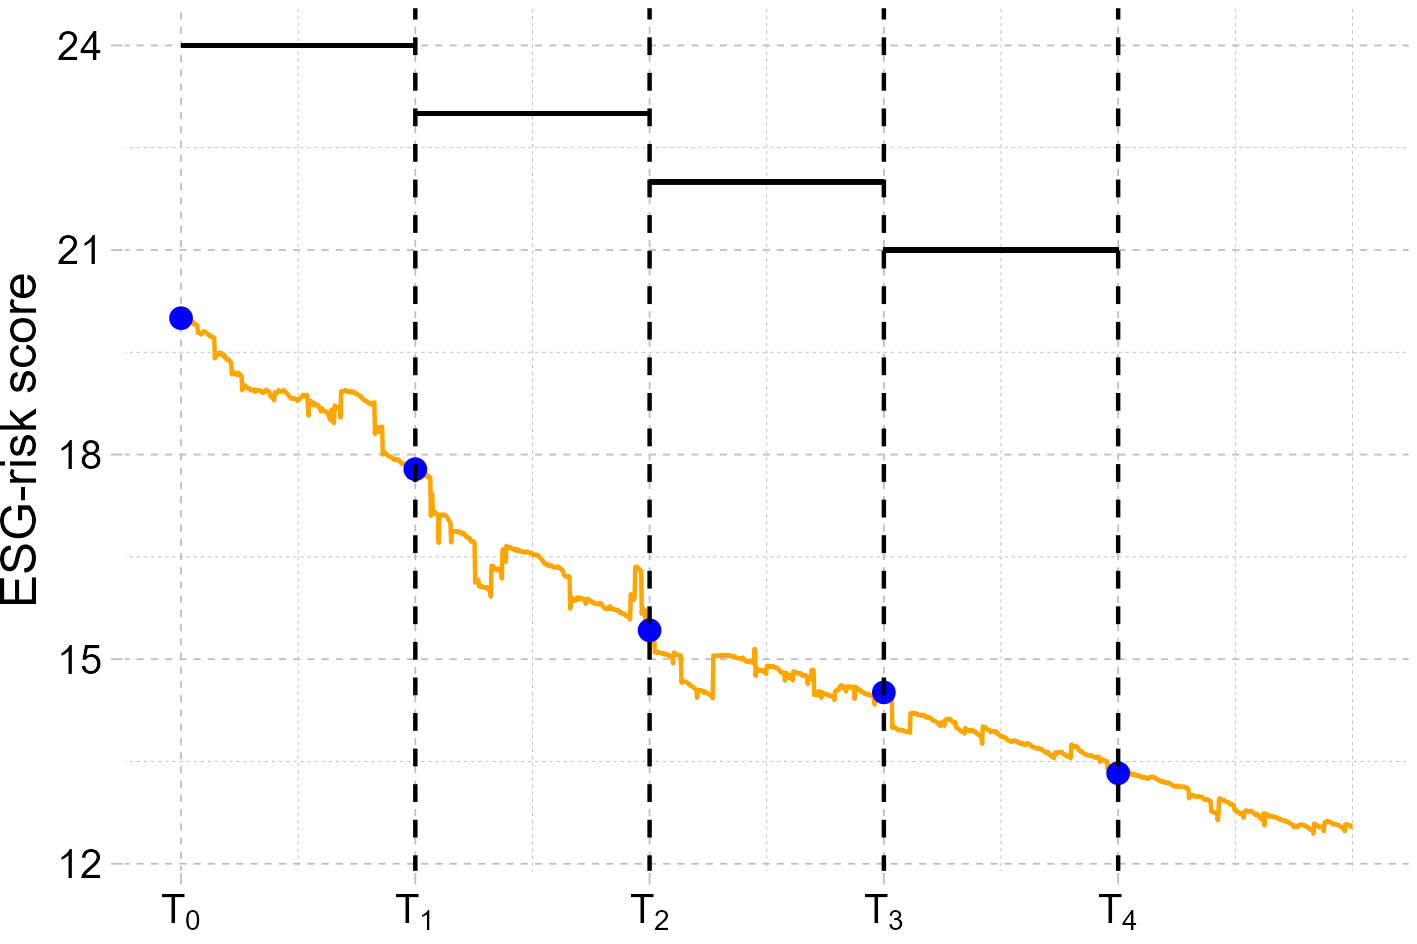
\includegraphics[width= 9cm]{figures/ESG/ESG_plt_criteria2.png}
    \caption{ESG-risk score where ESG-criteria is met often}
    \label{fig: ESG-risk_score_criteri2}
\end{figure}

In this particular we met the criteria at all time points $T_{i}$ for $i=1,2,3$. 


\begin{center}
    \begin{tabular}{ | l | l | l | p{5cm} |}
    \hline
    Time    & Criteria   & $\kappa_{t}^{ESG}(i)$ \\ \hline
    $T_{1}$ &   18       & $0.01046$  \\ \hline
    $T_{2}$ &   17       & $0.00876$  \\ \hline
    $T_{3}$ &   16       & $0.00605$\\ \hline
    $T_{4}$ &   15       & $0.00273$ \\ \hline
    \end{tabular}
\end{center} 

\begin{figure}[htp]
    \centering
    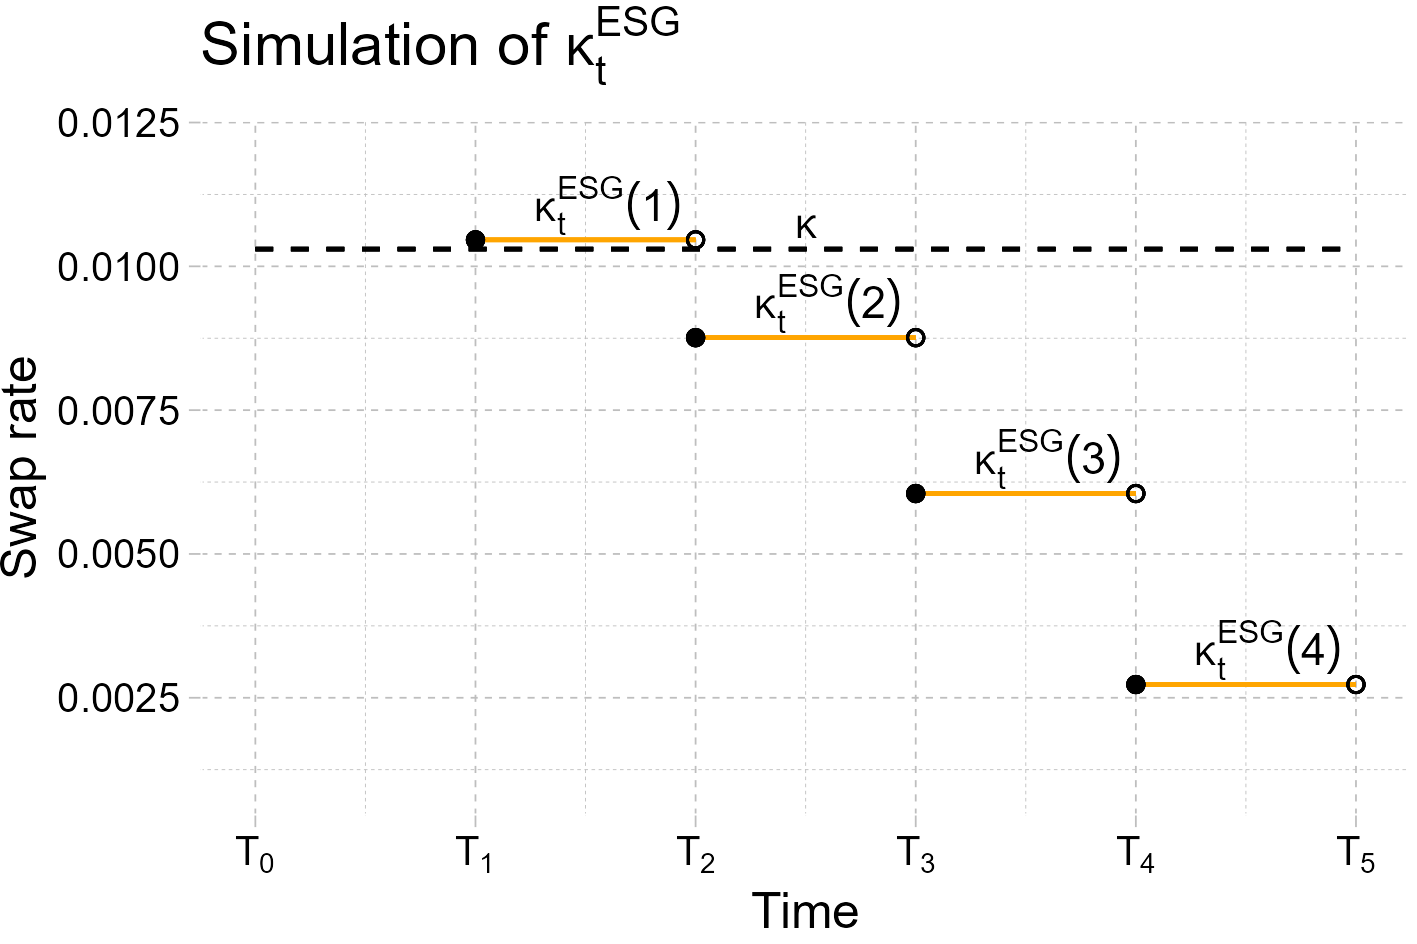
\includegraphics[width= 10cm]{figures/ESG/kappa_t_ESG_2.png}
    \caption{Meeting criteria often}
    \label{fig: ESG_swap_2}
\end{figure}

In this simulation, we got almost the swap rate at time $T_{1}$, and then the company met the criteria for $i=2,3,4$, giving a lower fixed rate. 


\newpage
\textbf{Never meeting criteria}
\\~\\ 
In this simulation we took: $C^{ESG} = 2.5$, for all timepoints and got: 

\begin{figure}[htp]
    \centering
    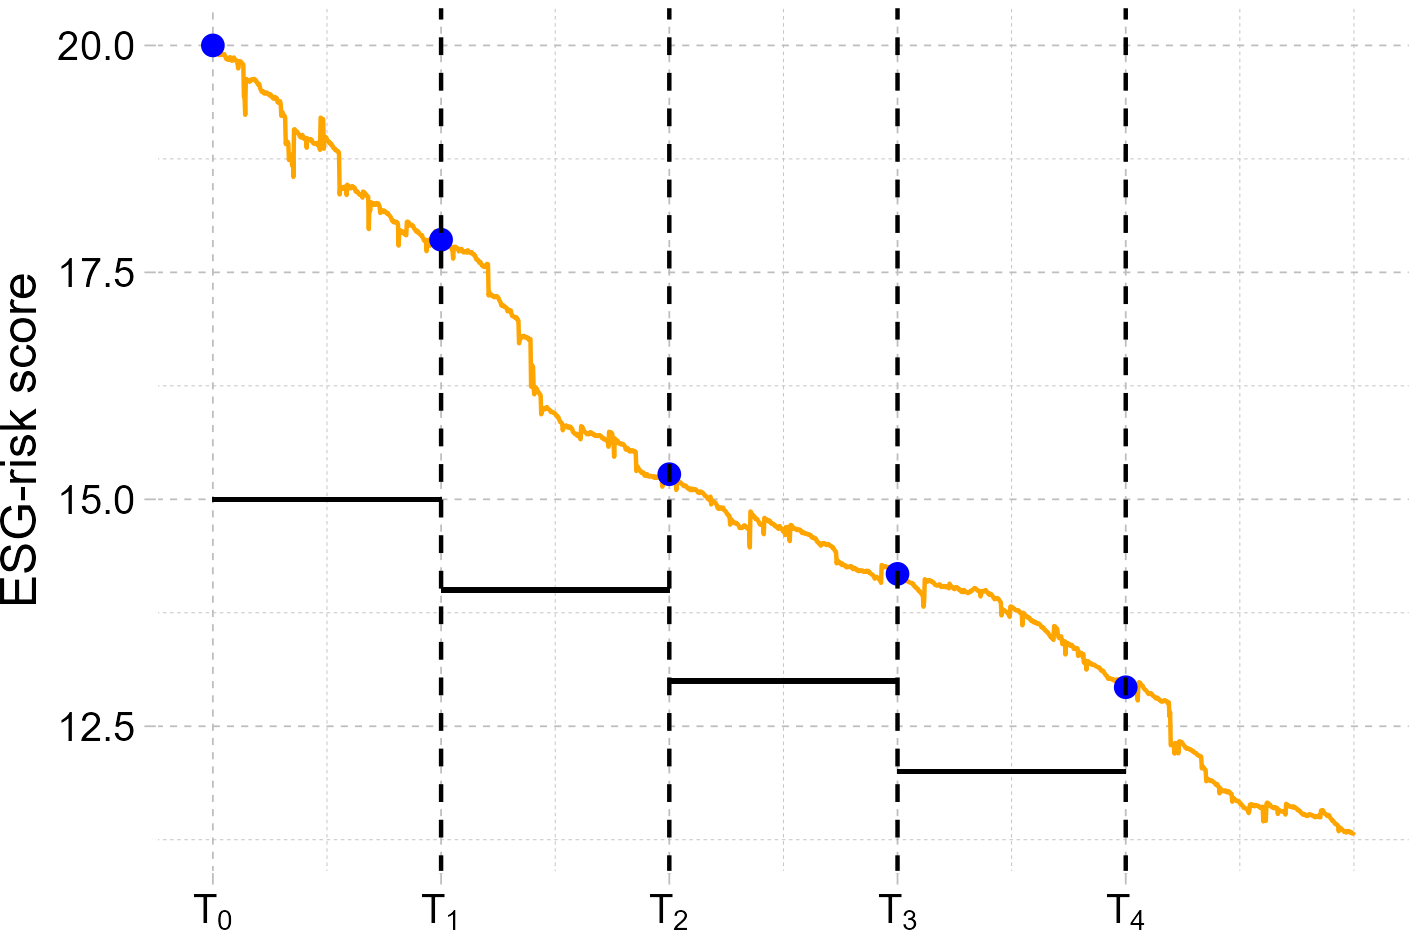
\includegraphics[width=9cm]{figures/ESG/ESG_plt_criteria3.png}
    \caption{ESG-risk score where ESG-criteria is never met}
    \label{fig: ESG-risk_score_criteria3}
\end{figure}




\begin{center}
    \begin{tabular}{ | l | l | l | p{5cm} |}
    \hline
    Time    & Criteria  & $\kappa_{t}^{ESG}(i)$ \\ \hline
    $T_{1}$ &    2.5    & $0.0153$  \\ \hline
    $T_{2}$ &    2.5    & $0.0203$  \\ \hline
    $T_{3}$ &    2.5    & $0.0253$\\ \hline
    $T_{4}$ &    2.5    & $0.0303$ \\ \hline
    \end{tabular}
\end{center} 


\begin{figure}[htp]
    \centering
    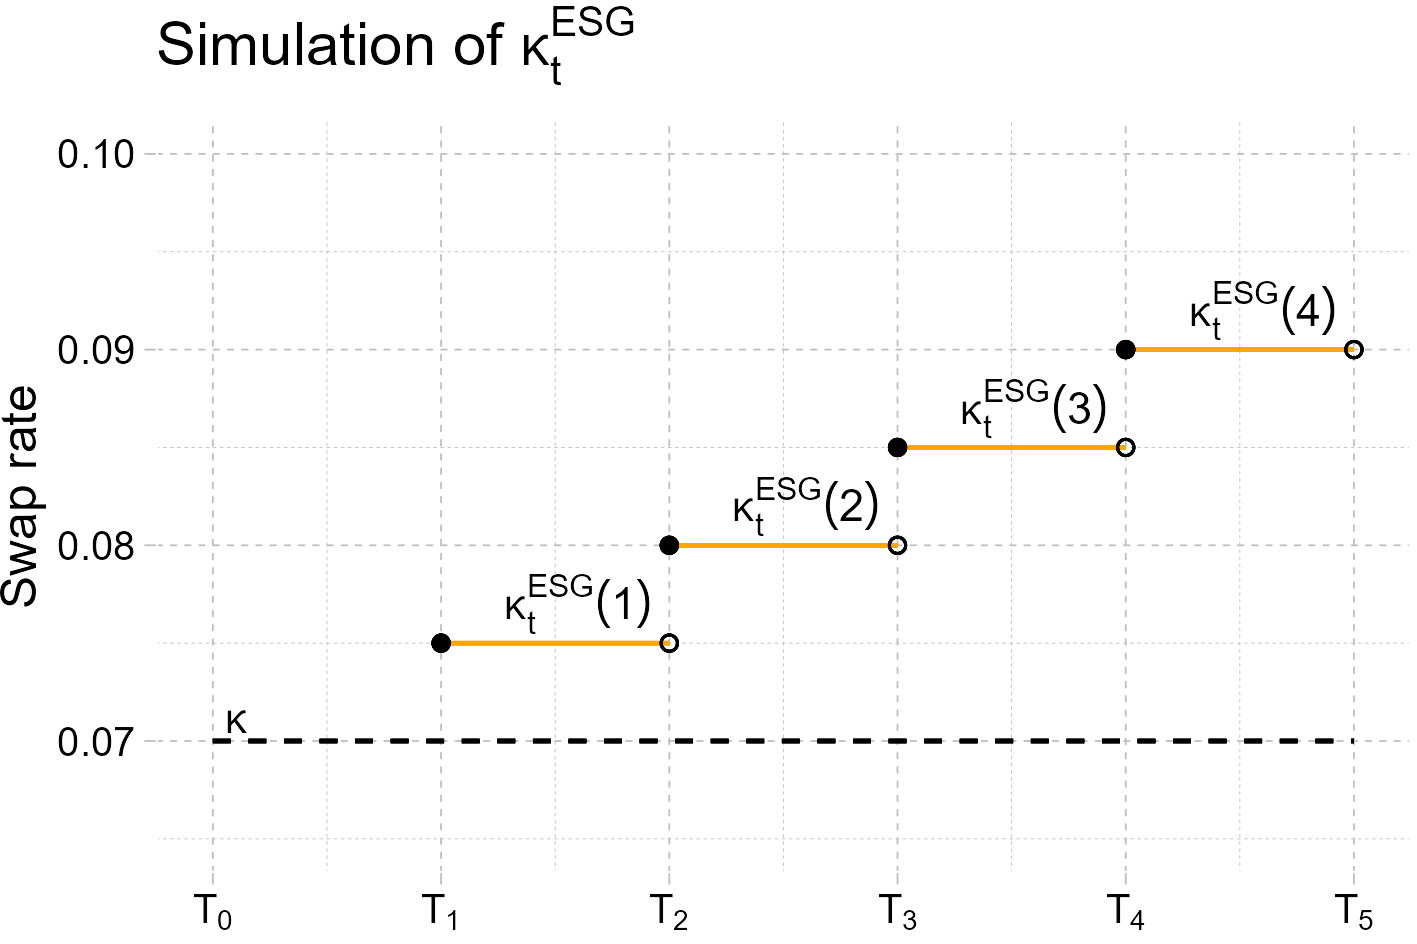
\includegraphics[width=10cm]{figures/ESG/kappa_t_ESG_3.png}
    \caption{ESG swap rate when ESG-criteria is never met}
    \label{fig: ESG_swap_3}
\end{figure} 

We see the effect of the penalty $d = 0.005$, leading to an upward-trending ESG swap rate. 










%\chapter{SOFR hedges}

\section{Hedging 3-month arithmetic with 3-month geometric}
Consider the case where we want to hedge: 
$$
X^{3M\_A} = \frac{1}{T-S}\int_{S}^{T}r_{u}du
$$

Here $[S,T]$ will denote a 3-month period, in the market we only have available
3-month futures $f^{3M}(t,S,T)$ (\ref{def: 3M_SOFR_futures})  calculated using a geometric average, this means that our hedge will look like: 
\begin{align*}
\argmin\limits_{a \in \R}\E_{Q}\left[
\left(
X^{3M\_A}-af^{3M}(t,S,T)
\right)^{2}
\bigg{|}\F_{t}
\right]
\end{align*}

Let's denote $H(a) :=\E_{Q}\left[
\left(X^{3M\_A}-af^{3M}(t,S,T)
\right)^{2}
\bigg{|}\F_{t}
\right]
$ 
expanding the square yields:
\begin{align*}
H(a) &= \E_{Q}\left[(X^{3M\_A})^{2}|\F_{t}\right] -2af^{3M}(t,S,T) +
a^{2}[f^{3M}(t,S,T)]^{2}
\end{align*}
Taking the derivative w.r.t. $a$ yields: 
\begin{align*}
H'(a) &= -2f^{3M}(t,S,T) + 2a[f^{3M}(t,S,T)]^{2}  
\end{align*} 

Now as $H''(a) = 2[f^{3M}(t,S,T)]^{2} > 0$, we have that the minimum is obtained by setting $H'(a) = 0$:
\begin{align*}
H'(a) &= 0 \\ 
&\Downarrow \\ 
a &= \frac{
\E_{Q}[X^{3M\_A}|\F_{t}]
}{
f^{3M}(t,S,T)
} \\ 
&= \frac{
\int_{S}^{T}\E_{Q}[r(u)|\F_{t}]du
}{
(T-S)f^{3M}(t,S,T)
}
\end{align*}

\begin{result}
Considering the above situation, we then have the following:
\begin{align*}
\argmin\limits_{a \in \R}\E_{Q}\left[
\left(
X^{3M\_A}-af^{3M}(t,S,T)
\right)^{2}
\bigg{|}\F_{t}
\right] 
\implies
a = \frac{
\int_{S}^{T}\E_{Q}[r(u)|\F_{t}]du
}{
(T-S)f^{3M}(t,S,T)
}
\end{align*}
\end{result} 

\newpage 

\subsection{Affine Term Structure-setting}

\begin{proposition}
Consider the above setting, and let $r = (r_{t})_{t\geq 0}$ be a model that provides ATS, then 
\begin{align*}
\argmin\limits_{a \in \R}&\E_{Q}\left[
\left(
X^{3M\_A}- af^{3M}(t,S,T)
\right)^{2}
\bigg{|}\F_{t}
\right] \\
&\Downarrow \\
a &= \frac{
r(t)(T-S)
+ \int_{S}^{T}\int_{t}^{u}b(s)dsdu 
+ \int_{S}^{T}\int_{t}^{u}\alpha(s)g(s)dsdu
}{
(T-S)f^{3M}(t,S,T)
}
\end{align*}
Where:
\begin{align*}
g(s) &= \exp\left(
\int_{t}^{s}\beta(v)dv
\right)
\left(
\int_{t}^{s}e^{-\int_{t}^{w}\beta(v)dv}b(w)dw + \E_{Q}[r(t)]
\right) 
\end{align*}
\end{proposition}

\begin{proof}
Consider the above setting, but now we assume that $r = (r_{t})_{t\geq 0}$ is a model that provides ATS (Affine Term Structure), now as described in proposition \ref{prop: condition_on_r_ATS}, we have that the dynamics of $r$ can be written as: 
\begin{align*}
dr(t) &= [b(t) + \beta(t)r(t)]dt + \sqrt{a(t) + \alpha(t)r(t)}dW^{Q}(t)
\end{align*}
Here $b, \beta, a, \alpha$ are deterministic continuous functions. Now from the dynamics, we get that for $u\geq t$: 
\begin{align*}
r(u) &= r(t) + \int_{t}^{u}b(s)ds + \int_{t}^{u}[\beta(s)r(s)]ds
+ \int_{t}^{u}\sqrt{\alpha(s)}dW^{Q}(s)
+ \int_{t}^{u}\sqrt{\alpha(s)r(s)}dW^{Q}(s)
\end{align*}

Each term is assumed to be Ito-integrable, i.e in $M^{2}([0,T])$, and by \\ $\F_{t}$-independence, we get:
\begin{align*}
\E_{Q}\left[
\int_{t}^{u}\sqrt{\alpha(s)}dW^{Q}(s)
\right]
&= 0 \\ 
\E_{Q}\left[
\int_{t}^{u}\sqrt{\alpha(s)r(s)}dW^{Q}(s)
\right] 
&= 0
\end{align*} 

And by using Stochastic-Fubini(\ref{thm: Stochastic_Fubini}), we get:
\begin{align*}
\E_{Q}\left[
\int_{t}^{u}[\beta(s)r(s)]ds
\right]
&= 
\int_{t}^{u}\beta(s)\E_{Q}[r(s)]ds
\end{align*}

This leaves us with: 
\begin{align*}
\int_{S}^{T}\E_{Q}[r(u)|\F_{t}]du 
&= r(t)(T-S)
+ \int_{S}^{T}\int_{t}^{u}b(s)dsdu 
+ \int_{S}^{T}\int_{t}^{u}\alpha(s)\E_{Q}[r(s)]dsdu
\end{align*}


\textbf{Overview of time-interval:}


\begin{tikzpicture}[snake=zigzag, line before snake = 5mm, line after snake = 5mm]
    % draw horizontal line   
    \draw (0,0) -- (9,0);
    %\draw[snake] (2,0) -- (4,0);
    %\draw (4,0) -- (5,0);
    %\draw[snake] (5,0) -- (7,0);
    %\draw[snake] (7,0) -- (9,0);
    %\draw (9,0) -- (10,0);

    % draw vertical lines
    \foreach \x in {0,2,4,5,7}
      \draw (\x cm,3pt) -- (\x cm,-3pt);

    % draw nodes
    \draw (0,0) node[below=3pt] {$ t $} node[above=3pt] {$   $};
    %\draw (1,0) node[below=3pt] {$ T_{0} $} node[above=3pt] {$  $};
    \draw (2,0) node[below=3pt] {$ S $} node[above=3pt] {$  $};
    %\draw (3,0) node[below=3pt] {$  $} node[above=3pt] {$  $};
    \draw (4,0) node[below=3pt] {$ s $} node[above=3pt] {$  $};
    \draw (5,0) node[below=3pt] {$ u $} node[above=3pt] {$  $};
    \draw (6,0) node[below=3pt] {$  $} node[above=3pt] {$  $};
    \draw (7,0) node[below=3pt] {$ T $} node[above=3pt] {$ $};
    %\draw (9,0) node[below=3pt] {$ T_{M} $} node[above=3pt] {$ $};
\end{tikzpicture} 
  
Thus in our setting we have: $t\leq S \leq s \leq u \leq T$, using same argument as above: 

\begin{align*}
r(s) &= r(t) + \int_{t}^{s}b(v)dv + \int_{t}^{s}[\beta(v)r(v)]dv
+ \int_{t}^{s}\sqrt{\alpha(v)}dW^{Q}(v)
+ \int_{t}^{s}\sqrt{\alpha(v)r(v)}dW^{Q}(v)    
\end{align*}

Now let $g(s) := \E_{Q}[r(s)]$: 
\begin{align*}
g(s) &= r(t) + \int_{t}^{s}b(v)dv + \int_{t}^{s}\beta(v)\E_{Q}[r(v)]dv
\end{align*}

Now taking the derivative w.r.t. $s$ and using the fundamental theorem of calculus, we get: 
\begin{align*}
g'(s) &= b(s) + \beta(s)\E_{Q}[r(s)] \\ 
&= b(s) + \beta(s)g(s), \; g(t) = \E_{Q}[r(t)]
\end{align*}

This is an ordinary differential equation, with the explicit solution given by:
\begin{align*}
 g(s) &= \exp\left(
 \int_{t}^{s}\beta(v)dv
 \right)
 \left(
 \int_{t}^{s}e^{-\int_{t}^{w}\beta(v)dv}b(w)dw + \E_{Q}[r(t)]
 \right)
\end{align*}
\end{proof}


\subsection{Hedging with available instruments in the market}

We now denote: 
\begin{align*}
X^{3M\_A} &= \frac{1}{T-S}\int_{S}^{T}r_{u}du = \frac{1}{T-S}Z \\ 
f^{3M\_A}(t,S,T) &= \frac{1}{T-S}\E_{Q}\left[
\int_{S}^{T}r_{u}du
\right] = \frac{1}{T-S}\E_{Q}[Z|\F_{t}]
\end{align*}

Now from Jensen's Inequality \ref{thm: Jensen's_ineuality}, we have that for $Z, \varphi(Z) \in L^{1}(\Omega, \F, Q)$, with $\varphi(x) = e^{x}$
\begin{align}
\label{eq: hedging_availible_inst_market_1}
\exp\left(
\E_{Q}[Z|\F_{t}]
\right)
&\leq 
\E_{Q}\left[
\exp(Z)|\F_{t}
\right] \nonumber \\ 
&\Updownarrow \nonumber \\ 
\exp\left(
(T-S)f^{3M\_A}(t,S,T)
\right) 
&\leq 
\E_{Q}\left[\exp(Z)|\F_{t}\right]
\end{align} 

Now from definition \ref{def: 3M_SOFR_futures}, we have: 
\begin{align}
\label{eq: hedging_availible_inst_market_2}
f^{3M}(t,S,T) &= \frac{1}{T-S}\left(
\E_{Q}\left[
\underbrace{e^{\int_{S}^{T}r_{u}du}}_{e^{Z}}
\bigg{|}\F_{t}\right] - 1
\right) \nonumber \\ 
&\Downarrow \nonumber \\ 
\E_{Q}[\exp(Z)|\F_{t}] &= (T-S)f^{3M}(t,S,T) + 1
\end{align}

Now by inserting \ref{eq: hedging_availible_inst_market_2} into \ref{eq: hedging_availible_inst_market_1} yields:

\begin{align*}
\exp\left(
(T-S)f^{3M\_A}(t,S,T)
\right) 
&\leq 
(T-S)f^{3M}(t,S,T) + 1 \\ 
&\Updownarrow \\
f^{3M\_A}(t,S,T) &\leq 
\frac{
\ln[(T-S)f^{3M}(t,S,T)]
}{
(T-S)
}
\end{align*}
%\include{chapters/results}
\chapter{Discussion and Conclusion}

In the SOFR studies, we examined the implications of different underlying calculation methods for the SOFR futures. We studied a 3M-arithmetic product: 
\[
X^{3M_{A}}(S,T) = \frac{1}{T-S}\int_{S}^{T}r_{u}du
\]
Against taking  a $\hat{a}_{t}-f^{3M}(t,S,T)$ 3M-SOFR futures position vs \\ 
taking  a $(\hat{a}_{t}, \hat{b}_{t}, \hat{c}_{t})-f^{1M}(t,S,T)$ 1M-SOFR futures position.  
\\~\\
For simulation purposes, we chose the following model for the integral of $r = (r(t))_{t\geq 0}$: 
\begin{align*}
\int_{S}^{T}r(u)du 
&= 
\left(
\frac{r(t)-m}{\alpha}
\right)
\left[
e^{-\alpha(S-t)} - e^{-\alpha(T-t)}
\right]
+ m(T-S) 
+ 
\frac{\sigma}{\alpha}\int_{t}^{T}\Sigma(u,t,S,T)dW^{Q}(u)   
\end{align*}
Where: 
\begin{align*}
\Sigma(u,t,S,T) &= 
\left[
e^{-\alpha(S-u)}-e^{-\alpha(T-u)}
\right]\mathbbm{1}_{[t,S)}(u) 
+ 
\left[
1-e^{-\alpha(T-u)}
\right]\mathbbm{1}_{[S,T]}(u)
\end{align*}

It should be mentioned that this may not be a realistic representation of $r$, and should be addressed accordingly. As mentioned in \cite{brigo2013interest}, a solution could be multi-factor models, as one source of uncertainty could be too restrictive for realistic modelling approaches.
\\~\\
In \cite{Skov_2020}, they consider 1-, 2- and 3-factor versions of Gaussian arbitrage-free short-rate models. One should also take into account the market price of risk $\lambda_{t}$, coming from Girsanov's Theorem: $dW^{Q}(t) = dW(t) - \lambda_{t}dt$, to get suitable  $P$-dynamics of the futures rates: $f^{\ell M}, \ell = 1,3$
\\~\\
From simulations we got $\hat{a}_{t}^{3M} = 0.95$ for the position in 3M-SOFR futures. An ideal hedge here would be if this number equalled $1$. Pretend that instead of hedging $X^{3M_{A}}(S,T)$, we wanted to hedge: 
\begin{align*}
X^{3M_{G}}(S,T) := \frac{1}{T-S}\left[
e^{\int_{S}^{T}r(u)du}-1
\right]    
\end{align*}

Namely a geometric average over the period $[S,T]$, then: 
\begin{align*}
G(a_{t}) := \argmin\limits_{a_{t} \in \R}\E_{Q}\left[
\left(
X^{3M_{G}}(S,T)-a_{t}f^{3M}(t,S,T)
\right)^{2}
\bigg{|}\F_{t}
\right]
\end{align*}

Now following the same arguments as on p.\pageref{result: optimal_SOFR_hedge_3MA_vs_3GM}, we get: 
\begin{align*}
\hat{a}_{t}^{3M} &= \frac{
\E_{Q}[X^{3M_{G}}(S,T)|\F_{t}]
}{
f^{3M}(t,S,T)
}
= 
\frac{
f^{3M}(t,S,T)
}{
f^{3M}(t,S,T)
} = 1
\end{align*}


\newpage 
We imposed a model for ESG-linked swaps, which lead to a sequence of fixed rates $\kappa_{t}^{ESG}  = (\kappa_{t}^{ESG}(i))_{i=1}^{n}$ giving a penalty/discount depending on whether the criteria were met or not.
\\~\\ 
We remember that the criteria $A_{i}$ looked like the following:
\begin{align*}
A_{i} &= \{X_{T_{i}} \leq C_{T_{i}}^{ESG}\}    
\end{align*}

This means that our ESG-fixed rate process heavily depends upon the OU-process $X(t)$ and the criteria $C_{T_{i}}^{ESG}$. It could be hard to establish "reasonable" criteria. In our simulation, we took $C^{ESG} = (C_{T_{i}}^{ESG})_{i\geq 1}$ to be $\F_{0}$-measurable, this could lead to some uncertainty as one would have to "know" even more about the company's development. Maybe a more reasonable approach would be to take $C^{ESG}$ to be $\F_{T_{i-1}}$-measurable. However, this would require a model for $C^{ESG}$, which adds to the complexity again.    
\\~\\
In our modelling approach, we modelled directly under $Q$. However, the market one operates in is under $P$, meaning that it would have been suitable with an Esscher-transform of $X(t)$, which then by  Proposition \ref{prop: Esscher_transform_CPP_Q} means that we would still have a CPP, but with altered intensity $\lambda_{Q}$ and jump-size distribution $F_{J}^{Q}(dx)$.
\\~\\
In our case we have $I(t) = \sum_{k=1}^{N(t)}J_{k}$ with $N(t) \sim Pois(\lambda t)$ and 
$J\sim Exp(\mu)$, and from Lemma \ref{lemma: CPP_exp_mu}, with $\theta \in (-\infty, \mu)$, we have:
\begin{align*}
\lambda_{Q} &= \frac{\lambda \mu}{\theta - \mu} \;\text{and}\;
J \stackrel{Q}{\sim} Exp(\mu - \theta)
\end{align*}

Furthermore, $X(t)$ is company dependent, meaning that to get reasonable estimates of the necessary parameters included, data accessibility is crucial to impose a suitable model. 
\\~\\ 
One should also mention that many ESG-rating agencies have different metrics for measuring the ESG score/risk score. These metrics are not necessarily standardized, and it can be unclear how the rating firm weighs the "E", "S", and "G". Should "E" be more "important" than "S" or "G"? 
\\~\\
If one looks at the expression $K_{n}^{ESG}(\omega)$: 
\begin{align*}
K_{n}^{ESG}(\omega) &= 
[\kappa -dn]\mathbbm{1}\left[
\bigcap_{i\in \mathcal{I}_{n}}A_{i}
\right](\omega) \\ 
&+ 
\sum_{\alpha \in \mathcal{I}_{2n}^{Even}}
\left(
[\kappa -d(n-\alpha)]\mathbbm{1}\left[
\bigcup_{
j_{1}\neq \dots \neq j_{|\mathcal{I}_{\alpha}^{Even}|}
\in \mathcal{I}_{n}
}\left(
\bigcap_{i\in \mathcal{I}_{n}}A_{i}
\right)^{
\{
(j_{1}, \dots , j_{|\mathcal{I}_{\alpha}^{Even}|})
\}
}
\right]
\right)(\omega) 
\end{align*}

We see that it tracks every path, and for each $n$ there are $2^{n}$-possible paths, meaning that as $n$ increases, the complexity increases. Furthermore, this expression is rather general, meaning that one must rely upon Monte Carlo simulations to get an estimate of $\kappa_{t}^{ESG}(i)$. At the same time, it also gives possibilities for other types of stochastic models for the ESG-risk score. 




%\label{discussion}
%\kant[15] % Dummy text
%\section{All my great results}
%\kant[16]
%\paragraph{List with bullets}
%\begin{itemize}
%    \item This is a list with bullets - the symbol can be %changed easily.
%     \item[!] A point to exclaim something!
%  \item[$\blacksquare$] Make the point fair and square.
%  \item[] A blank label?
%    \item This is the last item.
%\end{itemize}
%\paragraph{Numbered lists}
%\begin{enumerate}
%    \item This is a numbered list.
%     \item This is the second item.
%\end{enumerate}
%\paragraph{Descriptions}
%\begin{description}
%\item[My first great result] This is a description list.
% \item[My second great result] This is the second item.
%\end{description}
%\section{Pros and cons}
%\kant[17]
%\section{Future research}
%\kant[18]

\chapter{Conclusion}
\label{conc}



\kant[17] % Dummy text
%\chapter{Abbreviations and Symbols}

%\textbf{Abbreviations}
%\begin{itemize}[label={}]
%\item \textbf{1M}  1-month
%\item \textbf{3M}  3-months
%\item \textbf{ATS} Affine Term Structure
%\item \textbf{CPP} Compound Poisson Process
%\item \textbf{DCT} Dominated Convergence Theorem
%\item \textbf{ESG} Environmental, Social and Governance
%\item \textbf{HJM} Heath-Jarrow-Morton
%\item \textbf{LIBOR} London Interbank Offered Rate
%\end{itemize} 

Here are some abbreviations:

\nomenclature{ESG}{Environmental, Social, and Governance}
\nomenclature{CPP}{Compound}

%\printnomenclature


 
\printbibliography[heading=bibintoc,title={References}]
\printnomenclature[2.5cm]

\backmatter{}
    \appendix % "Chapter" is renamed "Appendix"
    %\begin{refsection}
    \chapter{Scripts}
%New colors defined below
\definecolor{codegreen}{rgb}{0,0.6,0}
\definecolor{codegray}{rgb}{0.5,0.5,0.5}
\definecolor{codepurple}{rgb}{0.58,0,0.82}
\definecolor{backcolour}{rgb}{0.95,0.95,0.92}

%Code listing style named "mystyle"
\lstdefinestyle{mystyle}{
  backgroundcolor=\color{backcolour}, commentstyle=\color{codegreen},
  keywordstyle=\color{magenta},
  numberstyle=\tiny\color{codegray},
  stringstyle=\color{codepurple},
  basicstyle=\ttfamily\footnotesize,
  breakatwhitespace=false,         
  breaklines=true,                 
  captionpos=b,                    
  keepspaces=true,                 
  numbers=left,                    
  numbersep=5pt,                  
  showspaces=false,                
  showstringspaces=false,
  showtabs=false,                  
  tabsize=2
}

%\section{R-code to generate ESG-fixed rate path}
%\lstset{style=mystyle}
%\lstinputlisting[language = R, caption = {Estimating Term Structure}]{scripts/R/SBM_ESG_process.R}


%\section{R-code to generate Term Structure}
%\lstset{style=mystyle}
%\lstinputlisting[language = R, caption = {Estimating Term Structure}]{scripts/R/Nelson_Siegel.R}


%\newpage 

%\section{R-code to generate ESG-figures}
%\lstset{style=mystyle}
%\lstinputlisting[language = R, caption = {Generate ESG-risk score}]{scripts/R/criteria_plt.R}
\section{SOFR: Simulation of $\kappa_{t}^{3M-SOFR}$}
\begin{minted}{julia}
#statistics and distributions
using Random 
using Distributions
using Statistics

#data-wrangeling:
using DataFrames

#for numerical integration:
using QuadGK

#plotting histogram and LaTeX labels:
using Plots 
using LaTeXStrings

#---------------------------------------------------------------------
#time parameters
T0 = 1/12
T1 = 4/12
T2 = 7/12
T3 = 10/12
timepoints = [T0, T1, T2, T3]
n_steps = 10000

#We use that Vasicek is ATS, i.e P(t,T) = exp(-A(t,T)-B(t,T)r(t))

function r_Vasicek(alpha, m,sigma, r_t, time_interval, n_steps)
    """
    Args: 
        #Vasicek parameters:
        alpha (Float): speed of reversion 
        m (float): long term mean level 
        sigma (float): volatility 
        r_t (float): initial value of r = (r(u))
        
        #time:
        time_interval (vector): the time interval we model over e.g [0,3]
        n_steps (int): number of timesteps we partition over
    
    Returns: 
        it simulates the process: r = (r(u)), for u in [t_start, t_end]
    """

    #time partition: 
    t_start = time_interval[1]
    t_end = time_interval[2]
    dt = (t_end-t_start)/n_steps
    n_steps = length(collect(t_start:dt:t_end))

    #initializing r: 
    r = zeros(n_steps)
    r[1] = r_t

    #Standard normal rv's
    Z = rand(Normal(0,1), n_steps)

    for i in 2:n_steps
        r[i] = r[i-1] - alpha*(m-r[i-1])*dt + sigma*Z[i]*dt
    end

    return r
end

function B_ZCB(t,T)
    ans = -(1/alpha)*(exp(-alpha*(T-t))-1)
    return ans
end

function A_ZCB(t,T)
    integral, _ = quadgk(u -> B_ZCB(u,T)^(2), t,T)
    ans = m*B_ZCB(t,T) - m*(T-t) - (1/2)*sigma^(2)*integral 
    return ans
end

function P(t,T, r_t)
    ans = exp(-A_ZCB(t,T) -B_ZCB(t,T)*r_t)
    return ans
end

#--------------------------------------------------------------
#Calculating f^3M(t,S,T), again using ATS structure:
#f^3M(t,S,T) = 1/(T-S)*(exp(A(t,S,T) + B(t,S,T)r(t))-1)
function Sigma1(u,t,S,T)
    ans = exp(-alpha*(S-u)) - exp(-alpha*(T-u))
    return ans   
end

function Sigma2(u,t,S,T)
    ans = 1-exp(-alpha*(T-u))
    return ans
end

function B(t,S,T)
    ans = (1/alpha)*(exp(-alpha*(S-t))-exp(-alpha*(T-t)))
    return ans
end

function A(t,S,T)
    first_part = m*(T-S) - m*B(t,S,T)
    c1_2, _  = quadgk(u -> Sigma1(u, t, t, S)^(2), t,S) 
    c2_2, _  = quadgk(u -> Sigma2(u, t, S, T)^(2), S,T)

    ans = first_part + (1/2)*(sigma^2/alpha^2)*(c1_2 + c2_2)

    return ans
end


function f_3M(t,S,T, r_t)
    ans = (1/(T-S))*(exp(A(t,S,T) + B(t,S,T)*r_t) - 1)
    return ans
end 

#time t-value of kappa in SOFR-swap
function kappa_t(t, r_t)
    "
    Args: 
        t (float): a vector of time points i.e [0,T1]
        r_t (float): vector of realization of interest rate model
    Returns: 
        the fixed swap rate kappa_t_3M-SOFR
    "
    ZCB_prices = map(T -> P(t,T, r_t), timepoints[2:end])
    f_3M_rates = map((x, y) -> f_3M(t, x, y, r_t), timepoints[1:end-1], timepoints[2:end])
    above = sum(ZCB_prices.*f_3M_rates)
    below = sum(ZCB_prices) 
    ans = above/below
    return ans
end


function kappa_path(t, r)
    "
    Args: 
        t (float): vector of timepoints 
        r (float): vector of desired interest rate model
    Returns: 
        vector of (t,r_t)-valued kappa_t
    "
    ans = map((x, y) -> kappa_t(x, y), t, r)
    return ans
end

#Vasicek parameters: 
alpha = 0.25
m = 0.035
r_0 = 0.0425
sigma = 0.05

r_0 = 0.0425
t_start = 0 
t_end = T0

r = r_Vasicek(alpha, m, sigma, r_0, [t_start,t_end], n_steps)
dt = (t_end-t_start)/n_steps
t = collect(t_start:dt:t_end)

length(r)
n_sim = 10
M = zeros(length(r), n_sim)
R = zeros(length(r), n_sim)


Random.seed!(1234)
for i in 1:n_sim
    r = r_Vasicek(alpha, m, sigma, r_0, [t_start,t_end], n_steps)
    kappa = kappa_path(t,r)
    R[:, i] = r
    M[:, i] = kappa
end
M
R

plot(R, layout = (1,1), 
        legend = false,
        title = L"t \mapsto r(t),\alpha = 0.25, m = 0.035, \sigma = 0.05, r_{0} = 0.0425 "
        )
xticks!([0, 10_000/2 ,10_000], ["0", L"\frac{T_{0}}{2}", L"T_{0}"])


# plot each column of the matrix
plot(M, layout=(1,1), 
        legend = false, 
        title = L"t \mapsto \kappa_{t}^{3M-SOFR},\alpha = 0.25, m = 0.035, \sigma = 0.05, r_{0} = 0.0425"
        )
xticks!([0, 10_000/2 ,10_000], ["0", L"\frac{T_{0}}{2}", L"T_{0}"])


\end{minted}

\newpage 

\section{SOFR: Hedging 3M-arithmetic SOFR}
\begin{minted}{julia}
using Random 
using Distributions
using Statistics

#for matrix operations and linear programming
using LinearAlgebra
using JuMP  #lp-problem setup
using HiGHS #lp-solver

#data-wrangeling:
using DataFrames

#for numerical integration:
using QuadGK

#plotting histogram and LaTeX labels:
using Plots 
using LaTeXStrings

#--------------------------------------------------------------------------#
#Vasicek parameters: 
alpha = 0.25
m = 0.035
r_t = 0.0425
sigma = 0.02

#time parameters
t = 0
S = 1/12
T1M = 2/12
T2M = 3/12
T = 4/12

function Sigma1(u,t,S,T)
    ans = exp(-alpha*(S-u)) - exp(-alpha*(T-u))
    return ans   
end


function Sigma2(u,t,S,T)
    ans = 1-exp(-alpha*(T-u))
    return ans
end


function int_r_start_stop(low,up, t)
    "
    Args: 
        low: (float), lower integration limit
        up: (float), upper integtation limit
    Returns: 
        the integral: int_low_up r(u)du
    "
    if t > low
        return "Please chose t <=low"
    end

    #Sigma1 is N(0, int_t_low c1_2 du), Sigma2 is N(0, int_low_up c2_2 du)
    c1_2, _  = quadgk(u -> Sigma1(u, t, low,up)^(2), t,low) 
    c2_2, _  = quadgk(u -> Sigma2(u, t, low,up)^(2), low,up)
    
    c1 = sqrt(c1_2)
    c2 = sqrt(c2_2)
    Z = rand(Normal(0,1))
    ans = ((r_t-m)/alpha)*(exp(-alpha*(low-t))-exp(-alpha*(up-t))) + m*(up-low) + sigma/alpha*(c1*Z + c2*Z)
    return ans
end


function integrand_E_Q_r(u, r_t, t)
    ans = exp(-alpha*(u-t))*r_t + m*(1-exp(-alpha*(u-t)))
    return ans
end

#int_S_T E_Q[r(u)|F_t]du:
integral_E_Q_r, _ = quadgk(u -> integrand_E_Q_r(u, r_t, t), S,T)

integral_E_Q_r
#--------------------------------------------------------------------------#
# Calculating a_hat_3M:

function B(t,S,T)
    ans = (1/alpha)*(exp(-alpha*(S-t))-exp(-alpha*(T-t)))
    return ans
end

function A(t,S,T)
    first_part = m*(T-S) - m*B(t,S,T)
    c1_2, _  = quadgk(u -> Sigma1(u, t, t, S)^(2), t,S) 
    c2_2, _  = quadgk(u -> Sigma2(u, t, S, T)^(2), S,T)

    ans = first_part + (1/2)*(sigma^2/alpha^2)*(c1_2 + c2_2)

    return ans
end


function f_3M(t,S,T)
    ans = (1/(T-S))*(exp(A(t,S,T) + B(t,S,T)*r_t) - 1)
    return ans
end

f_3M(0,S,T)

a_hat = integral_E_Q_r/((T-S)*f_3M(0,S,T))

#-------------------------------------------------------------------------------------------#
# 3M-arithmetic vs (a,b,c) 1M-SOFR futures: 
integral1 , _ = quadgk(u -> integrand_E_Q_r(u, r_t, t), S,T1M)
integral2 , _ = quadgk(u -> integrand_E_Q_r(u, r_t, t), T1M,T2M)
integral3 , _ = quadgk(u -> integrand_E_Q_r(u, r_t, t), T2M,T)

f_1M_S_T1M = (1/(T1M-S))*integral1
f_1M_T1M_T2M = (1/(T2M-T1M))*integral2
f_1M_T2M_T = (1/(T-T2M))*integral3

#variable naming to be more consistent with MSc Thesis:
a = f_1M_S_T1M        #alpha, I use alpha in Vasicek, hence a: 
beta = f_1M_T1M_T2M   #beta
gamma = f_1M_T2M_T    #gamma

futures = [a,beta,gamma]

#E_Q[X^(3M_A)(S,T)|F_t] = q: 
q = (1/(T-S))*integral_E_Q_r 

#matrix of coeff: 
M = [a^(2)      a*beta  a*gamma;
     beta^(2)   a*beta  beta*gamma; 
     gamma^(2)  a*beta  beta*gamma] 
     
#vector of values: 
b = q.*[a;
        beta;
        gamma] 

#optimal weight of futures:
x_hat = inv(M)*b 
#-------------------------------------------------------------------------------------------#
# incase M is not invertible: 
# Define optimization problem
model = Model(HiGHS.Optimizer)
@variable(model, x[1:3])
@objective(model, Min, sum(x))
@constraint(model, M * x .== b)
@constraint(model, -1 .<= x .<= 1 )
abs.([1,2,-3])
# Solve optimization problem
optimize!(model)
# optimal value
x_tilde = value.(x)

#-------------------------------------------------------------------------------------------#
# Simulations: 
n_sim = 10^(6)
#constants: 
#int_S_T E_Q[r(u)|F_t]du:
integral_E_Q_r, _ = quadgk(u -> integrand_E_Q_r(u, r_t, t), S,T)

futures_weighted_M_inv = x_hat'futures
futures_weighted_BP = x_tilde'futures
futures_weighted_one_each = [1,1,1]'futures

X_3MA = zeros(n_sim)
for i in 1:n_sim
    #aritmetic interest rate relaization:
    X_3MA[i] = (1/(T-S))*(int_r_start_stop(S,T,t))
end

X_3MA
#elementwise substraction:
ER_1 = X_3MA .-(1/(T-S))*integral_E_Q_r
ER_2_M_inv = X_3MA .-futures_weighted_M_inv
ER_2_111 = X_3MA .-futures_weighted_one_each



#-----------------------------------------------------------
# plotting of histograms: 
mean_ER_1 = mean(ER_1)
mean_ER_1 = round(mean_ER_1, digits = 3)

sigma_ER_1 = std(ER_1) 
sigma_ER_1 = round(sigma_ER_1, digits = 2)

mean_ER_2_M_inv = mean(ER_2_M_inv)
mean_ER_2_M_inv = round(mean_ER_2_M_inv, digits = 3)

sigma_ER_2 = std(ER_2_M_inv)
sigma_ER_2 = round(sigma_ER_2_M_inv, digits = 2)

mean_ER_2_111 = mean(ER_2_111)
mean_ER_2_111 = round(mean_ER_2_111,digits =3)

sigma_ER_2_111 = std(ER_2_111)
sigma_ER_2_111 = round(sigma_ER_2_111, digits = 2)

#ER_1
histogram(ER_1, 
          color =:lightblue, 
          xlabel="Value", 
          ylabel="Frequency", 
          title = L"Histogram\; of\; ER_{1}(0), \; s_{ER_{1}}\approx 0.01,\;n_{sim} = 10^{6}", 
          labels = "ER_1(0)", 
          xticks = [-3*sigma_ER_1, -2*sigma_ER_1,-sigma_ER_1, mean_ER_1,  sigma_ER_1, 2*sigma_ER_1, 3*sigma_ER_1]
          )
vline!([mean_ER_1], lw = 5, labels = L"mean(ER_{1}(0))" )


#ER_2_M_inv:
histogram(ER_2_M_inv, 
          color =:lightblue, 
          xlabel="Value", 
          ylabel="Frequency", 
          title = L"Histogram\; of\; ER_{2}^{M_{inv}}(0), \; s_{ER_{2}^{M_{inv}}} \approx 0.01, \;n_{sim} = 10^{6}", 
          labels = L"ER_{2}^{M_{inv}}(0)", 
          xticks = [-3*sigma_ER_2, -2*sigma_ER_2,-sigma_ER_2, mean_ER_2_M_inv, sigma_ER_2, 2*sigma_ER_2, 3*sigma_ER_2]
          )
vline!([mean_ER_2_M_inv], lw = 5, labels = L"mean(ER_{2}^{M_{inv}}(0))")

#(1,1,1)-weight of futures:
histogram(ER_2_111, 
          color =:lightblue, 
          xlabel="Value", 
          ylabel="Frequency", 
          title = L"Histogram\; of\; ER_{2}^{(1,1,1)}(0), \; s_{ER_{2}^{(1,1,1)}} \approx 0.01, \;n_{sim} = 10^{6}", 
          labels = L"ER_{2}^{(1,1,1)}(0)", 
          xticks = [-12*sigma_ER_2_111,-10*sigma_ER_2_111, mean_ER_2_111, -7*sigma_ER_2_111, -5*sigma_ER_2_111])
vline!([mean_ER_2_one_each], lw = 5, labels =  L"mean(ER_{2}^{(1,1,1)}(0))")
\end{minted}

\newpage 

\section{Numerical Simulation For ESG swap rate}

\begin{minted}{julia}
using Random 
using Distributions
using Statistics

using LinearAlgebra
using Queryverse
using DataFrames

using Combinatorics
using Plots

function create_array(dims::Array{Tuple{Int,Int},1})
    "
    Args: 
        dims: (array(tuple)), vector of tuples, 
              where each element corresponds to matrix-dimension
    
    Returns:
        Array of matricies A = (M_1, …, M_n)
        Each matrix can take on different dimensions, i.e:
        dimensions = [(m,n), (k,l), (r,q), ...] 
        The array will return matricies of zeros    
    "
    arr = Array{Array{Float64,2}}(undef, length(dims))

    for (i, dim) in enumerate(dims)
        arr[i] = zeros(dim...)
    end

    return(arr)
end

function all_perm(xs, n)
    " 
    Args: 
        xs: (Vector)
        n: (Int), desired length
    
    Returns:
        generates permutation of elements in vector xs of length n
        all_perm([0.0, 1.0], 2) = [0.0, 0.0],[1.0, 0.0], [0.0, 1.0], [1.0, 1.0]
        all_perm([0.0, 1.0], 3) = [0.0, 0.0, 0.0], [0.0, 1.0, 0.0], [1.0, 0.0, 0.0], ...
    "
    return(vec(map(collect, Iterators.product(ntuple(_ -> xs, n)...))))
end 


function OU_CPP(z0::Float64, beta::Float64, sigma::Float64, lambda::Float64, mu::Float64, dt::Float64,T_end::Float64)
    " 
    Description:
        dZ(t) = -beta*Z(t)dt + sigma*dW(t) + dI(t)
        I(t): I(t) = sum_{i=1}^{N(t)}J_k, J_k ~ Exp(mu), 
        NB! Julia parametrize with 1/mu

    Args:    
        z0: (float) inital value of the process Z(t)
        beta: (float), mean-retreving parameter
        sigma: (float), parameter of Brownian Motion
        lambda: (float), jump intensity of process, N(t)~ Pois(lambda*t) 
        dt: (float) stepsize 
        T_end: (float), for how long the simulation should go
     
    Returns: 
        X(t) = 100exp(-Z(t))
    "

    time = collect(0:dt:T_end) 
    n = length(time)

    #number of jumps from [0,T_end] on each dt: N(dt) ~ Pois(lambda*dt)
    N = rand(Poisson(lambda*dt),n) 

    #Brownian motion W~N(0,dt) on [0,dt]
    W = rand(Normal(0,1) ,n)

    #intialising Z(t)
    z = zeros(n)

    z[1] = z0

    #dZ(t) = -beta*Z(t)dt + sigma*dW(t) + dI(t)
    for i in 2:n 
        dI = sum(rand(Exponential(mu), N[i])) - sum(rand(Exponential(mu), N[i-1]))
        z[i] = z[i-1] - beta*z[i-1]*dt + sigma*W[i]*dt + dI
    end

    #X(t) = 100exp(-Z(t))
    x = 100*exp.(-z)
    df = DataFrame(time = time, score = x)
    return df
end

function simulation(n_sim, C_ESG, T_end, relevant_times)
    "
    Args:
        n_sim: (int) number of simulations 
        C_ESG: Vector(float) ESG-criteria at time T_{i}            
        relevant_times: (float) vector of relevant times, 
        [T1, T2, T3, ...], percentage of year.
    "

    "
    retruns:
        matrix of wheter or not criteria is meet
        each row in the matrix corresponds to a simulation, i.e
        m = [0,0,0; did not meet any criteria
             0,1,1; met criteria at T2 and T3
             ...  ] 
    "
    
    #store matrix of zeros, row = simulation number, col = agreed observation times
    m = zeros(n_sim, length(relevant_times))
    for i in 1:n_sim
        #df_tmp: general simulation 
        df_tmp = OU_CPP(-log(20/100), -0.05, 0.0,20.0, 1/150.0,1/360, T_end)
        #get the relevant timepoints as df:
        df_relevant = filter(row -> row.time in relevant_times, df_tmp)
        #get the score:
        relevant_score = df_relevant.score
    
        #check if X_{T_{i}} <= C^_{T_{i}}^{ESG} for T_{1}, ..., T_{n}
        ESG_criteria = relevant_score .<= C_ESG 
        ESG_criteria = Float64.(ESG_criteria)
        
        #store ESG_criteria:
        m[i, :] = ESG_criteria
    end

    return(m)
end

function D(i::Int, m::Matrix)
    " 
    Args:
        i: (Int), index in sequence 
        m: (Matrix), matrix containing simulations

    Returns: 
        D(i)-term in in E_{Q}[K_{i}^{ESG}(omega)|F_{t}]    
    "
    if i > size(m)[2]
        return println("You cannot evaluate D outside of agreed contract")
    end
    
    #adjusting for column dimensions in Boolean check:
    m_adj = m[:, 1:i]

    v = all_perm([0.0, 1.0], i)
    possible_patterns = mapreduce(permutedims, vcat, v)
    
    #use the row sum to determine how many errors/fails there are:
    success_sum = collect(0.0:Float64(i))
    
    #p is the indicator of successes for the trial:
    p = zeros(size(possible_patterns)[1], i+1)
    for k in 1:(i+1)
        p[:, k] = Bool[success_sum[k] == sum(possible_patterns[j, :]) for j=1:size(possible_patterns,1)]'
    end
    #turn p into Boolean object so that we can use findall:
    p = Bool.(p)

    #store row dimensions, so that we can initialize array later
    row_dims = zeros(Int, i+1)
    for i in 1:(i+1)
        row_dims[i] = size(possible_patterns[findall(p[:, i]), :])[1]
    end
    
    #initializing the needed dimensions
    dimensions = [(row_dims[k], i) for k in 1:(i+1)] 
    " 
    A: array of matricies, A=(M_1, ..., M_i)
    Let i = 3:
    M_1: matrix of patterns giving zero successes  [0,0,0] (1x3)
    M_2: matrix of patterns giving one succeses    [0,0,1;
                                                    0,1,0; 
                                                    1,0,0] (3x3)
    M_3: matrix of patterns giving two succeses    [1,1,0;
                                                    1,0,1;
                                                    0,1,1] (3x3)                                                
    etc. 
    "
    A = create_array(dimensions) 

    for l in 1:(i+1)
        A[l] = possible_patterns[findall(p[:, l]), :]
    end

    " 
    E_fails: (vector) Expecation of all linear combinations where: 
    E_fails[1]: expectation of all linear combinations giving all fails (1 path)
    E_fails[2]: expectation of all linear combinaition giving fails, but 1 success (multiple paths)
    Let i=3: E_fails[1] = E[fff|F_t]
             E_fails[2] = E[ssf|F_t] + E[sfs|F_t] + E[fss|F_t]
    etc.
    "
    E_fails = zeros(i+1)

    for l in 1:(i+1)
        s = 0 
        for j in 1:size(A[l],1)
            s += mean(Bool[A[l][j, :] == m_adj[r, :] for r=1:size(m_adj,1)])
        end
        E_fails[l] = s
    end 
    
    #represents I_{2i}^{Even} = {2,...,2i}
    I_2_Even = collect(2.0:2.0:Float64(2*i))

    #represents vector of sum_{alpha in I_{2i}^{Even}}[i-alpha], 
    weight = i .- I_2_Even

    #all success, all success but one, all success but two, ... 
    E_success = reverse(E_fails)
    
    #=
    i*E_{Q}[\cap 1(A_{l})|F_t] + 
    sum_[alpha \in I_2_Even]sum_[j_1 != ... != j_I_alpha_Even]x
    E_{Q}[(\cap 1(A_{l}))^[[j_{1} != ... != j_I_alpha_Even]]|F_t] 
    =#

    ans = i*E_success[1] + sum(weight.*E_success[2:length(E_success)])

    return(ans)
end

relevant_times = [1.25, 2.25, 3.25, 4.25]

C_ESG = [17.6, 16.6, 15.6, 14.55]
m = simulation(10^(6), C_ESG, 4.25, relevant_times)


#----------------------------------------------------------------------------
#kappa_{t}^{ESG} and kappa_{t}: 
#Calculating kappa for the above example:

#constants:
d = 0.005 #discount
delta = 1.00  #equidistant distance between T_{i} and T_{i-1}
num_steps = 1:length(relevant_times) #number of relevant steps

#ZCB:
P_T0 = 0.995
P_T1 = 0.985
P_T2 = 0.975
P_T3 = 0.965
P_T4 = 0.955

#vector of ZCB
P = [P_T0, P_T1, P_T2, P_T3, P_T4] 

#ordinary fixed rate kappa form ZCB-swap
kappa_t_ZCB = (P[1]-P[length(P)])/(delta*sum(P[2:length(P)]))

#the ESG-Swap process:
function kappa_t_ESG(i)
    kappa_t_ZCB-d*D(i,m)
end

println("(t, kappa_t_ZCB, kappa_t_ESG, C_ESG, relevant_times)")
for i in 1:length(relevant_times)
    println((i, kappa_t_ZCB ,kappa_t_ESG(i), C_ESG, relevant_times))
end


#meet criteria often:  
C_ESG_2 = [18, 17, 16, 15]
m2 = simulation(10^(5), C_ESG_2, 4.25, relevant_times)

function kappa_t_ESG_2(i)
    kappa_t_ZCB-d*D(i,m2)
end

for i in 1:length(relevant_times)
    println((i, kappa_t_ZCB ,kappa_t_ESG_2(i), C_ESG_2, relevant_times))
end

#does not meet criteria: 
C_ESG_3 = 2.5

m3 = simulation(10^(5), C_ESG_3, 4.25, relevant_times)

function kappa_t_ESG_3(i)
    kappa_t_ZCB-d*D(i,m3)
end

for i in 1:length(relevant_times)
    println((i, kappa_t_ZCB ,kappa_t_ESG_3(i), C_ESG_3, relevant_times))
end


\end{minted}


%\lstset{style=mystyle}
%\lstinputlisting[language = julia, caption = {ESG-swap rate Simulation}]{ZCB_ESG_for_latex.jl}

%\jlinputlisting{ZCB_ESG_for_latex.jl}

%\lstinputlisting[language= Julia]{ZCB_ESG_for_latex.jl}


% displayed code
%\begin{jllisting}
%# some julia code
%println( "Here we go with Julia!")
%\end{jllisting}

    \chapter{Scripts}
%New colors defined below
\definecolor{codegreen}{rgb}{0,0.6,0}
\definecolor{codegray}{rgb}{0.5,0.5,0.5}
\definecolor{codepurple}{rgb}{0.58,0,0.82}
\definecolor{backcolour}{rgb}{0.95,0.95,0.92}

%Code listing style named "mystyle"
\lstdefinestyle{mystyle}{
  backgroundcolor=\color{backcolour}, commentstyle=\color{codegreen},
  keywordstyle=\color{magenta},
  numberstyle=\tiny\color{codegray},
  stringstyle=\color{codepurple},
  basicstyle=\ttfamily\footnotesize,
  breakatwhitespace=false,         
  breaklines=true,                 
  captionpos=b,                    
  keepspaces=true,                 
  numbers=left,                    
  numbersep=5pt,                  
  showspaces=false,                
  showstringspaces=false,
  showtabs=false,                  
  tabsize=2
}

%\section{R-code to generate ESG-fixed rate path}
%\lstset{style=mystyle}
%\lstinputlisting[language = R, caption = {Estimating Term Structure}]{scripts/R/SBM_ESG_process.R}


%\section{R-code to generate Term Structure}
%\lstset{style=mystyle}
%\lstinputlisting[language = R, caption = {Estimating Term Structure}]{scripts/R/Nelson_Siegel.R}


%\newpage 

%\section{R-code to generate ESG-figures}
%\lstset{style=mystyle}
%\lstinputlisting[language = R, caption = {Generate ESG-risk score}]{scripts/R/criteria_plt.R}
\section{SOFR: Simulation of $\kappa_{t}^{3M-SOFR}$}
\begin{minted}{julia}
#statistics and distributions
using Random 
using Distributions
using Statistics

#data-wrangeling:
using DataFrames

#for numerical integration:
using QuadGK

#plotting histogram and LaTeX labels:
using Plots 
using LaTeXStrings

#---------------------------------------------------------------------
#time parameters
T0 = 1/12
T1 = 4/12
T2 = 7/12
T3 = 10/12
timepoints = [T0, T1, T2, T3]
n_steps = 10000

#We use that Vasicek is ATS, i.e P(t,T) = exp(-A(t,T)-B(t,T)r(t))

function r_Vasicek(alpha, m,sigma, r_t, time_interval, n_steps)
    """
    Args: 
        #Vasicek parameters:
        alpha (Float): speed of reversion 
        m (float): long term mean level 
        sigma (float): volatility 
        r_t (float): initial value of r = (r(u))
        
        #time:
        time_interval (vector): the time interval we model over e.g [0,3]
        n_steps (int): number of timesteps we partition over
    
    Returns: 
        it simulates the process: r = (r(u)), for u in [t_start, t_end]
    """

    #time partition: 
    t_start = time_interval[1]
    t_end = time_interval[2]
    dt = (t_end-t_start)/n_steps
    n_steps = length(collect(t_start:dt:t_end))

    #initializing r: 
    r = zeros(n_steps)
    r[1] = r_t

    #Standard normal rv's
    Z = rand(Normal(0,1), n_steps)

    for i in 2:n_steps
        r[i] = r[i-1] - alpha*(m-r[i-1])*dt + sigma*Z[i]*dt
    end

    return r
end

function B_ZCB(t,T)
    ans = -(1/alpha)*(exp(-alpha*(T-t))-1)
    return ans
end

function A_ZCB(t,T)
    integral, _ = quadgk(u -> B_ZCB(u,T)^(2), t,T)
    ans = m*B_ZCB(t,T) - m*(T-t) - (1/2)*sigma^(2)*integral 
    return ans
end

function P(t,T, r_t)
    ans = exp(-A_ZCB(t,T) -B_ZCB(t,T)*r_t)
    return ans
end

#--------------------------------------------------------------
#Calculating f^3M(t,S,T), again using ATS structure:
#f^3M(t,S,T) = 1/(T-S)*(exp(A(t,S,T) + B(t,S,T)r(t))-1)
function Sigma1(u,t,S,T)
    ans = exp(-alpha*(S-u)) - exp(-alpha*(T-u))
    return ans   
end

function Sigma2(u,t,S,T)
    ans = 1-exp(-alpha*(T-u))
    return ans
end

function B(t,S,T)
    ans = (1/alpha)*(exp(-alpha*(S-t))-exp(-alpha*(T-t)))
    return ans
end

function A(t,S,T)
    first_part = m*(T-S) - m*B(t,S,T)
    c1_2, _  = quadgk(u -> Sigma1(u, t, t, S)^(2), t,S) 
    c2_2, _  = quadgk(u -> Sigma2(u, t, S, T)^(2), S,T)

    ans = first_part + (1/2)*(sigma^2/alpha^2)*(c1_2 + c2_2)

    return ans
end


function f_3M(t,S,T, r_t)
    ans = (1/(T-S))*(exp(A(t,S,T) + B(t,S,T)*r_t) - 1)
    return ans
end 

#time t-value of kappa in SOFR-swap
function kappa_t(t, r_t)
    "
    Args: 
        t (float): a vector of time points i.e [0,T1]
        r_t (float): vector of realization of interest rate model
    Returns: 
        the fixed swap rate kappa_t_3M-SOFR
    "
    ZCB_prices = map(T -> P(t,T, r_t), timepoints[2:end])
    f_3M_rates = map((x, y) -> f_3M(t, x, y, r_t), timepoints[1:end-1], timepoints[2:end])
    above = sum(ZCB_prices.*f_3M_rates)
    below = sum(ZCB_prices) 
    ans = above/below
    return ans
end


function kappa_path(t, r)
    "
    Args: 
        t (float): vector of timepoints 
        r (float): vector of desired interest rate model
    Returns: 
        vector of (t,r_t)-valued kappa_t
    "
    ans = map((x, y) -> kappa_t(x, y), t, r)
    return ans
end

#Vasicek parameters: 
alpha = 0.25
m = 0.035
r_0 = 0.0425
sigma = 0.05

r_0 = 0.0425
t_start = 0 
t_end = T0

r = r_Vasicek(alpha, m, sigma, r_0, [t_start,t_end], n_steps)
dt = (t_end-t_start)/n_steps
t = collect(t_start:dt:t_end)

length(r)
n_sim = 10
M = zeros(length(r), n_sim)
R = zeros(length(r), n_sim)


Random.seed!(1234)
for i in 1:n_sim
    r = r_Vasicek(alpha, m, sigma, r_0, [t_start,t_end], n_steps)
    kappa = kappa_path(t,r)
    R[:, i] = r
    M[:, i] = kappa
end
M
R

plot(R, layout = (1,1), 
        legend = false,
        title = L"t \mapsto r(t),\alpha = 0.25, m = 0.035, \sigma = 0.05, r_{0} = 0.0425 "
        )
xticks!([0, 10_000/2 ,10_000], ["0", L"\frac{T_{0}}{2}", L"T_{0}"])


# plot each column of the matrix
plot(M, layout=(1,1), 
        legend = false, 
        title = L"t \mapsto \kappa_{t}^{3M-SOFR},\alpha = 0.25, m = 0.035, \sigma = 0.05, r_{0} = 0.0425"
        )
xticks!([0, 10_000/2 ,10_000], ["0", L"\frac{T_{0}}{2}", L"T_{0}"])


\end{minted}

\newpage 

\section{SOFR: Hedging 3M-arithmetic SOFR}
\begin{minted}{julia}
using Random 
using Distributions
using Statistics

#for matrix operations and linear programming
using LinearAlgebra
using JuMP  #lp-problem setup
using HiGHS #lp-solver

#data-wrangeling:
using DataFrames

#for numerical integration:
using QuadGK

#plotting histogram and LaTeX labels:
using Plots 
using LaTeXStrings

#--------------------------------------------------------------------------#
#Vasicek parameters: 
alpha = 0.25
m = 0.035
r_t = 0.0425
sigma = 0.02

#time parameters
t = 0
S = 1/12
T1M = 2/12
T2M = 3/12
T = 4/12

function Sigma1(u,t,S,T)
    ans = exp(-alpha*(S-u)) - exp(-alpha*(T-u))
    return ans   
end


function Sigma2(u,t,S,T)
    ans = 1-exp(-alpha*(T-u))
    return ans
end


function int_r_start_stop(low,up, t)
    "
    Args: 
        low: (float), lower integration limit
        up: (float), upper integtation limit
    Returns: 
        the integral: int_low_up r(u)du
    "
    if t > low
        return "Please chose t <=low"
    end

    #Sigma1 is N(0, int_t_low c1_2 du), Sigma2 is N(0, int_low_up c2_2 du)
    c1_2, _  = quadgk(u -> Sigma1(u, t, low,up)^(2), t,low) 
    c2_2, _  = quadgk(u -> Sigma2(u, t, low,up)^(2), low,up)
    
    c1 = sqrt(c1_2)
    c2 = sqrt(c2_2)
    Z = rand(Normal(0,1))
    ans = ((r_t-m)/alpha)*(exp(-alpha*(low-t))-exp(-alpha*(up-t))) + m*(up-low) + sigma/alpha*(c1*Z + c2*Z)
    return ans
end


function integrand_E_Q_r(u, r_t, t)
    ans = exp(-alpha*(u-t))*r_t + m*(1-exp(-alpha*(u-t)))
    return ans
end

#int_S_T E_Q[r(u)|F_t]du:
integral_E_Q_r, _ = quadgk(u -> integrand_E_Q_r(u, r_t, t), S,T)

integral_E_Q_r
#--------------------------------------------------------------------------#
# Calculating a_hat_3M:

function B(t,S,T)
    ans = (1/alpha)*(exp(-alpha*(S-t))-exp(-alpha*(T-t)))
    return ans
end

function A(t,S,T)
    first_part = m*(T-S) - m*B(t,S,T)
    c1_2, _  = quadgk(u -> Sigma1(u, t, t, S)^(2), t,S) 
    c2_2, _  = quadgk(u -> Sigma2(u, t, S, T)^(2), S,T)

    ans = first_part + (1/2)*(sigma^2/alpha^2)*(c1_2 + c2_2)

    return ans
end


function f_3M(t,S,T)
    ans = (1/(T-S))*(exp(A(t,S,T) + B(t,S,T)*r_t) - 1)
    return ans
end

f_3M(0,S,T)

a_hat = integral_E_Q_r/((T-S)*f_3M(0,S,T))

#-------------------------------------------------------------------------------------------#
# 3M-arithmetic vs (a,b,c) 1M-SOFR futures: 
integral1 , _ = quadgk(u -> integrand_E_Q_r(u, r_t, t), S,T1M)
integral2 , _ = quadgk(u -> integrand_E_Q_r(u, r_t, t), T1M,T2M)
integral3 , _ = quadgk(u -> integrand_E_Q_r(u, r_t, t), T2M,T)

f_1M_S_T1M = (1/(T1M-S))*integral1
f_1M_T1M_T2M = (1/(T2M-T1M))*integral2
f_1M_T2M_T = (1/(T-T2M))*integral3

#variable naming to be more consistent with MSc Thesis:
a = f_1M_S_T1M        #alpha, I use alpha in Vasicek, hence a: 
beta = f_1M_T1M_T2M   #beta
gamma = f_1M_T2M_T    #gamma

futures = [a,beta,gamma]

#E_Q[X^(3M_A)(S,T)|F_t] = q: 
q = (1/(T-S))*integral_E_Q_r 

#matrix of coeff: 
M = [a^(2)      a*beta  a*gamma;
     beta^(2)   a*beta  beta*gamma; 
     gamma^(2)  a*beta  beta*gamma] 
     
#vector of values: 
b = q.*[a;
        beta;
        gamma] 

#optimal weight of futures:
x_hat = inv(M)*b 
#-------------------------------------------------------------------------------------------#
# incase M is not invertible: 
# Define optimization problem
model = Model(HiGHS.Optimizer)
@variable(model, x[1:3])
@objective(model, Min, sum(x))
@constraint(model, M * x .== b)
@constraint(model, -1 .<= x .<= 1 )
abs.([1,2,-3])
# Solve optimization problem
optimize!(model)
# optimal value
x_tilde = value.(x)

#-------------------------------------------------------------------------------------------#
# Simulations: 
n_sim = 10^(6)
#constants: 
#int_S_T E_Q[r(u)|F_t]du:
integral_E_Q_r, _ = quadgk(u -> integrand_E_Q_r(u, r_t, t), S,T)

futures_weighted_M_inv = x_hat'futures
futures_weighted_BP = x_tilde'futures
futures_weighted_one_each = [1,1,1]'futures

X_3MA = zeros(n_sim)
for i in 1:n_sim
    #aritmetic interest rate relaization:
    X_3MA[i] = (1/(T-S))*(int_r_start_stop(S,T,t))
end

X_3MA
#elementwise substraction:
ER_1 = X_3MA .-(1/(T-S))*integral_E_Q_r
ER_2_M_inv = X_3MA .-futures_weighted_M_inv
ER_2_111 = X_3MA .-futures_weighted_one_each



#-----------------------------------------------------------
# plotting of histograms: 
mean_ER_1 = mean(ER_1)
mean_ER_1 = round(mean_ER_1, digits = 3)

sigma_ER_1 = std(ER_1) 
sigma_ER_1 = round(sigma_ER_1, digits = 2)

mean_ER_2_M_inv = mean(ER_2_M_inv)
mean_ER_2_M_inv = round(mean_ER_2_M_inv, digits = 3)

sigma_ER_2 = std(ER_2_M_inv)
sigma_ER_2 = round(sigma_ER_2_M_inv, digits = 2)

mean_ER_2_111 = mean(ER_2_111)
mean_ER_2_111 = round(mean_ER_2_111,digits =3)

sigma_ER_2_111 = std(ER_2_111)
sigma_ER_2_111 = round(sigma_ER_2_111, digits = 2)

#ER_1
histogram(ER_1, 
          color =:lightblue, 
          xlabel="Value", 
          ylabel="Frequency", 
          title = L"Histogram\; of\; ER_{1}(0), \; s_{ER_{1}}\approx 0.01,\;n_{sim} = 10^{6}", 
          labels = "ER_1(0)", 
          xticks = [-3*sigma_ER_1, -2*sigma_ER_1,-sigma_ER_1, mean_ER_1,  sigma_ER_1, 2*sigma_ER_1, 3*sigma_ER_1]
          )
vline!([mean_ER_1], lw = 5, labels = L"mean(ER_{1}(0))" )


#ER_2_M_inv:
histogram(ER_2_M_inv, 
          color =:lightblue, 
          xlabel="Value", 
          ylabel="Frequency", 
          title = L"Histogram\; of\; ER_{2}^{M_{inv}}(0), \; s_{ER_{2}^{M_{inv}}} \approx 0.01, \;n_{sim} = 10^{6}", 
          labels = L"ER_{2}^{M_{inv}}(0)", 
          xticks = [-3*sigma_ER_2, -2*sigma_ER_2,-sigma_ER_2, mean_ER_2_M_inv, sigma_ER_2, 2*sigma_ER_2, 3*sigma_ER_2]
          )
vline!([mean_ER_2_M_inv], lw = 5, labels = L"mean(ER_{2}^{M_{inv}}(0))")

#(1,1,1)-weight of futures:
histogram(ER_2_111, 
          color =:lightblue, 
          xlabel="Value", 
          ylabel="Frequency", 
          title = L"Histogram\; of\; ER_{2}^{(1,1,1)}(0), \; s_{ER_{2}^{(1,1,1)}} \approx 0.01, \;n_{sim} = 10^{6}", 
          labels = L"ER_{2}^{(1,1,1)}(0)", 
          xticks = [-12*sigma_ER_2_111,-10*sigma_ER_2_111, mean_ER_2_111, -7*sigma_ER_2_111, -5*sigma_ER_2_111])
vline!([mean_ER_2_one_each], lw = 5, labels =  L"mean(ER_{2}^{(1,1,1)}(0))")
\end{minted}

\newpage 

\section{Numerical Simulation For ESG swap rate}

\begin{minted}{julia}
using Random 
using Distributions
using Statistics

using LinearAlgebra
using Queryverse
using DataFrames

using Combinatorics
using Plots

function create_array(dims::Array{Tuple{Int,Int},1})
    "
    Args: 
        dims: (array(tuple)), vector of tuples, 
              where each element corresponds to matrix-dimension
    
    Returns:
        Array of matricies A = (M_1, …, M_n)
        Each matrix can take on different dimensions, i.e:
        dimensions = [(m,n), (k,l), (r,q), ...] 
        The array will return matricies of zeros    
    "
    arr = Array{Array{Float64,2}}(undef, length(dims))

    for (i, dim) in enumerate(dims)
        arr[i] = zeros(dim...)
    end

    return(arr)
end

function all_perm(xs, n)
    " 
    Args: 
        xs: (Vector)
        n: (Int), desired length
    
    Returns:
        generates permutation of elements in vector xs of length n
        all_perm([0.0, 1.0], 2) = [0.0, 0.0],[1.0, 0.0], [0.0, 1.0], [1.0, 1.0]
        all_perm([0.0, 1.0], 3) = [0.0, 0.0, 0.0], [0.0, 1.0, 0.0], [1.0, 0.0, 0.0], ...
    "
    return(vec(map(collect, Iterators.product(ntuple(_ -> xs, n)...))))
end 


function OU_CPP(z0::Float64, beta::Float64, sigma::Float64, lambda::Float64, mu::Float64, dt::Float64,T_end::Float64)
    " 
    Description:
        dZ(t) = -beta*Z(t)dt + sigma*dW(t) + dI(t)
        I(t): I(t) = sum_{i=1}^{N(t)}J_k, J_k ~ Exp(mu), 
        NB! Julia parametrize with 1/mu

    Args:    
        z0: (float) inital value of the process Z(t)
        beta: (float), mean-retreving parameter
        sigma: (float), parameter of Brownian Motion
        lambda: (float), jump intensity of process, N(t)~ Pois(lambda*t) 
        dt: (float) stepsize 
        T_end: (float), for how long the simulation should go
     
    Returns: 
        X(t) = 100exp(-Z(t))
    "

    time = collect(0:dt:T_end) 
    n = length(time)

    #number of jumps from [0,T_end] on each dt: N(dt) ~ Pois(lambda*dt)
    N = rand(Poisson(lambda*dt),n) 

    #Brownian motion W~N(0,dt) on [0,dt]
    W = rand(Normal(0,1) ,n)

    #intialising Z(t)
    z = zeros(n)

    z[1] = z0

    #dZ(t) = -beta*Z(t)dt + sigma*dW(t) + dI(t)
    for i in 2:n 
        dI = sum(rand(Exponential(mu), N[i])) - sum(rand(Exponential(mu), N[i-1]))
        z[i] = z[i-1] - beta*z[i-1]*dt + sigma*W[i]*dt + dI
    end

    #X(t) = 100exp(-Z(t))
    x = 100*exp.(-z)
    df = DataFrame(time = time, score = x)
    return df
end

function simulation(n_sim, C_ESG, T_end, relevant_times)
    "
    Args:
        n_sim: (int) number of simulations 
        C_ESG: Vector(float) ESG-criteria at time T_{i}            
        relevant_times: (float) vector of relevant times, 
        [T1, T2, T3, ...], percentage of year.
    "

    "
    retruns:
        matrix of wheter or not criteria is meet
        each row in the matrix corresponds to a simulation, i.e
        m = [0,0,0; did not meet any criteria
             0,1,1; met criteria at T2 and T3
             ...  ] 
    "
    
    #store matrix of zeros, row = simulation number, col = agreed observation times
    m = zeros(n_sim, length(relevant_times))
    for i in 1:n_sim
        #df_tmp: general simulation 
        df_tmp = OU_CPP(-log(20/100), -0.05, 0.0,20.0, 1/150.0,1/360, T_end)
        #get the relevant timepoints as df:
        df_relevant = filter(row -> row.time in relevant_times, df_tmp)
        #get the score:
        relevant_score = df_relevant.score
    
        #check if X_{T_{i}} <= C^_{T_{i}}^{ESG} for T_{1}, ..., T_{n}
        ESG_criteria = relevant_score .<= C_ESG 
        ESG_criteria = Float64.(ESG_criteria)
        
        #store ESG_criteria:
        m[i, :] = ESG_criteria
    end

    return(m)
end

function D(i::Int, m::Matrix)
    " 
    Args:
        i: (Int), index in sequence 
        m: (Matrix), matrix containing simulations

    Returns: 
        D(i)-term in in E_{Q}[K_{i}^{ESG}(omega)|F_{t}]    
    "
    if i > size(m)[2]
        return println("You cannot evaluate D outside of agreed contract")
    end
    
    #adjusting for column dimensions in Boolean check:
    m_adj = m[:, 1:i]

    v = all_perm([0.0, 1.0], i)
    possible_patterns = mapreduce(permutedims, vcat, v)
    
    #use the row sum to determine how many errors/fails there are:
    success_sum = collect(0.0:Float64(i))
    
    #p is the indicator of successes for the trial:
    p = zeros(size(possible_patterns)[1], i+1)
    for k in 1:(i+1)
        p[:, k] = Bool[success_sum[k] == sum(possible_patterns[j, :]) for j=1:size(possible_patterns,1)]'
    end
    #turn p into Boolean object so that we can use findall:
    p = Bool.(p)

    #store row dimensions, so that we can initialize array later
    row_dims = zeros(Int, i+1)
    for i in 1:(i+1)
        row_dims[i] = size(possible_patterns[findall(p[:, i]), :])[1]
    end
    
    #initializing the needed dimensions
    dimensions = [(row_dims[k], i) for k in 1:(i+1)] 
    " 
    A: array of matricies, A=(M_1, ..., M_i)
    Let i = 3:
    M_1: matrix of patterns giving zero successes  [0,0,0] (1x3)
    M_2: matrix of patterns giving one succeses    [0,0,1;
                                                    0,1,0; 
                                                    1,0,0] (3x3)
    M_3: matrix of patterns giving two succeses    [1,1,0;
                                                    1,0,1;
                                                    0,1,1] (3x3)                                                
    etc. 
    "
    A = create_array(dimensions) 

    for l in 1:(i+1)
        A[l] = possible_patterns[findall(p[:, l]), :]
    end

    " 
    E_fails: (vector) Expecation of all linear combinations where: 
    E_fails[1]: expectation of all linear combinations giving all fails (1 path)
    E_fails[2]: expectation of all linear combinaition giving fails, but 1 success (multiple paths)
    Let i=3: E_fails[1] = E[fff|F_t]
             E_fails[2] = E[ssf|F_t] + E[sfs|F_t] + E[fss|F_t]
    etc.
    "
    E_fails = zeros(i+1)

    for l in 1:(i+1)
        s = 0 
        for j in 1:size(A[l],1)
            s += mean(Bool[A[l][j, :] == m_adj[r, :] for r=1:size(m_adj,1)])
        end
        E_fails[l] = s
    end 
    
    #represents I_{2i}^{Even} = {2,...,2i}
    I_2_Even = collect(2.0:2.0:Float64(2*i))

    #represents vector of sum_{alpha in I_{2i}^{Even}}[i-alpha], 
    weight = i .- I_2_Even

    #all success, all success but one, all success but two, ... 
    E_success = reverse(E_fails)
    
    #=
    i*E_{Q}[\cap 1(A_{l})|F_t] + 
    sum_[alpha \in I_2_Even]sum_[j_1 != ... != j_I_alpha_Even]x
    E_{Q}[(\cap 1(A_{l}))^[[j_{1} != ... != j_I_alpha_Even]]|F_t] 
    =#

    ans = i*E_success[1] + sum(weight.*E_success[2:length(E_success)])

    return(ans)
end

relevant_times = [1.25, 2.25, 3.25, 4.25]

C_ESG = [17.6, 16.6, 15.6, 14.55]
m = simulation(10^(6), C_ESG, 4.25, relevant_times)


#----------------------------------------------------------------------------
#kappa_{t}^{ESG} and kappa_{t}: 
#Calculating kappa for the above example:

#constants:
d = 0.005 #discount
delta = 1.00  #equidistant distance between T_{i} and T_{i-1}
num_steps = 1:length(relevant_times) #number of relevant steps

#ZCB:
P_T0 = 0.995
P_T1 = 0.985
P_T2 = 0.975
P_T3 = 0.965
P_T4 = 0.955

#vector of ZCB
P = [P_T0, P_T1, P_T2, P_T3, P_T4] 

#ordinary fixed rate kappa form ZCB-swap
kappa_t_ZCB = (P[1]-P[length(P)])/(delta*sum(P[2:length(P)]))

#the ESG-Swap process:
function kappa_t_ESG(i)
    kappa_t_ZCB-d*D(i,m)
end

println("(t, kappa_t_ZCB, kappa_t_ESG, C_ESG, relevant_times)")
for i in 1:length(relevant_times)
    println((i, kappa_t_ZCB ,kappa_t_ESG(i), C_ESG, relevant_times))
end


#meet criteria often:  
C_ESG_2 = [18, 17, 16, 15]
m2 = simulation(10^(5), C_ESG_2, 4.25, relevant_times)

function kappa_t_ESG_2(i)
    kappa_t_ZCB-d*D(i,m2)
end

for i in 1:length(relevant_times)
    println((i, kappa_t_ZCB ,kappa_t_ESG_2(i), C_ESG_2, relevant_times))
end

#does not meet criteria: 
C_ESG_3 = 2.5

m3 = simulation(10^(5), C_ESG_3, 4.25, relevant_times)

function kappa_t_ESG_3(i)
    kappa_t_ZCB-d*D(i,m3)
end

for i in 1:length(relevant_times)
    println((i, kappa_t_ZCB ,kappa_t_ESG_3(i), C_ESG_3, relevant_times))
end


\end{minted}


%\lstset{style=mystyle}
%\lstinputlisting[language = julia, caption = {ESG-swap rate Simulation}]{ZCB_ESG_for_latex.jl}

%\jlinputlisting{ZCB_ESG_for_latex.jl}

%\lstinputlisting[language= Julia]{ZCB_ESG_for_latex.jl}


% displayed code
%\begin{jllisting}
%# some julia code
%println( "Here we go with Julia!")
%\end{jllisting}

%     \printbibliography[heading=bibintoc,title={References}]
%\end{refsection}
\end{document}